\documentclass[twocolumn]{aastex6}

%% The other main article choice is a tightly typeset, two-column article
%% that more closely resembles the final typeset pdf article.
%%
%% \documentclass[twocolumn]{aastex6}
%% 
%% There are other optional arguments one can envoke to allow other 
%% actions. 
%%
% These are the available options:
%   manuscript	: onecolumn, doublespace, 12pt fonts
%   preprint	: onecolumn, single space, 10pt fonts
%   preprint2	: twocolumn, single space, 10pt fonts
%   twocolumn	: a two column article. Probably not needed, but here just in case.
%   onecolumn	: a one column article; default option.
%   twocolappendix: make 2 column appendix
%   onecolappendix: make 1 column appendix is the default. 
%   astrosymb	: Loads Astrosymb font and define \astrocommands. 
%   tighten	: Makes baselineskip slightly smaller
%   times	: uses times font instead of the default
%   linenumbers	: turn on lineno package.
%   trackchanges : required to see the revision mark up and print output
%   numberedappendix: Labels appendix sections A, B, ... This is the default.
%   appendixfloats: Needed. Resets figure and table counters to zero

%% these can be used in any combination, e.g.
%%
%% \documentclass[twocolumn,twocolappendix,linenumbers,trackchanges]{aastex6}

\shorttitle{Galaxy Zoo: Hubble}
\shortauthors{Willett et al.}

%% This is the end of the preamble.  Indicate the beginning of the
%% paper itself with \begin{document}.

\usepackage{epsfig}
\usepackage{color,soul}
\usepackage{natbib}
\usepackage{amsmath,amssymb}
\usepackage{graphicx}
\usepackage{subfigure}
\usepackage{url}
\usepackage[normalem]{ulem}
\bibliographystyle{mn2e}

\newcommand{\s}{$_{\rm s}$}
\newcommand{\kms}{km~s$^{-1}$}
\newcommand{\msun}{{\it M}$_{\odot}$}
\newcommand{\lsun}{{\it L}$_{\odot}$}
\newcommand{\mear}{{\it M}$_{\oplus}$}
\newcommand{\etal}{{\it et al.}}
\newcommand{\ie}{{\it i.e.}}
\newcommand{\eg}{{\it e.g.}}
\newcommand{\be}{\begin{equation}}
\newcommand{\ee}{\end{equation}}
\newcommand{\magarc}{{\rm mag\,arcsec$^{-2}$}}
\newcommand{\MK}{{{\rm M}_{\rm ext,K}-5\log h}}
\newcommand{\ri}{{$r_{21}$}}
\newcommand{\ra}{$R_A$}
\newcommand{\vobs}{{v_{\rm obs}}}
\newcommand{\kmsMpc}{km~s$^{-1}$ Mpc$^{-1}$}
\newcommand{\h}{$h_{70}$}
\newcommand{\vpec}{v_{\rm pec}}
\newcommand{\like}{{\mathcal L}}
\newcommand{\vs}{\vspace*{5pt}}
\newcommand{\continued}{ (Continued)}

\newcommand{\ferengi}{\textsc{ferengi}}
\newcommand{\hst}{\textit{HST}}
\newcommand{\hubble}{\textit{Hubble Space Telescope}}
\newcommand{\subaru}{\textit{Subaru}}
\newcommand{\sextractor}{\textsc{SExtractor}}
\newcommand{\galapagos}{\textsc{Galapagos}}
\newcommand{\galfit}{\textsc{GALFIT}}
\newcommand{\gimtwod}{\textsc{GIM2D}}
\newcommand{\sersic}{S\'{e}rsic}


%\definecolor{titlecol}{rgb}{0,0,1}
%\definecolor{titlecol2}{rgb}{0,0.65,0}
\definecolor{titlecol3}{rgb}{1,0,0}
%
%\font\nbf=cmssbx10 at 12.28pt %big font for headers
%\def\note		{\color{titlecol3} \nbf}
\def\note		{\color{titlecol3}}




% Journals
%\newcommand{\mnras}{MNRAS}
%\newcommand{\apj}{ApJ}
%\newcommand{\apjl}{ApJL}
%\newcommand{\aj}{AJ}
%\newcommand{\pasp}{PASP}
%\newcommand{\aaps}{A\&AS}
%\newcommand{\aap}{A\&A}
%\newcommand{\apjs}{ApJS}
%\newcommand{\araa}{ARA\&A}

% Galaxy Zoo
\newcommand{\ffeatures}{$f_{\rm features}$}
\newcommand{\ffeaturesz}{$f_{\mathrm{features,}z}$}
\newcommand{\ffeaturesrest}{$f_{\mathrm{features,}z=0.3}$}
\newcommand{\ffeaturesdebiased}{$f_{\mathrm{features,debiased}}$}
\newcommand{\fbest}{$f_{\mathrm{features,best}}$}
\newcommand{\fodd}{$f_{\mathrm{odd}}$}
\newcommand{\fbar}{$f_{\mathrm{bar}}$}
\newcommand{\fsmooth}{$f_{\rm smooth}$}
\newcommand{\fartifact}{$f_{\rm artifact}$}

\newcommand{\fHI}{f_{\rm HI}}
\newcommand{\zsim}{$z_{\mathrm{sim}}$}

% Bands

\newcommand{\Bband}{$B_{435W}$}
\newcommand{\Vband}{$V_{606W}$}
\newcommand{\iband}{$I_{775W}$}
\newcommand{\Iband}{$I_{814W}$}
\newcommand{\zband}{$I_{850LP}$}

% Math

\DeclareMathOperator{\arcsinh}{arcsinh}



\begin{document}

%% LaTeX will automatically break titles if they run longer than
%% one line. However, you may use \\ to force a line break if
%% you desire.

\title{Galaxy Zoo: Morphological Classifications for 150,000 Galaxies in HST Legacy Imaging}
%% Use \author, \affil, plus the \and command to format author and affiliation 
%% information.  If done correctly the peer review system will be able to
%% automatically put the author and affiliation information from the manuscript
%% and save the corresponding author the trouble of entering it by hand.
%%
%% The \affil should be used to document primary affiliations and the
%% \altaffil should be used for secondary affiliations, titles, or email.

%% Authors with the same affiliation can be grouped in a single
%% \author and \affil call.
\author{Kyle W. Willett\altaffilmark{1,2}, Melanie A. Galloway\altaffilmark{1}, Chris J. Lintott\altaffilmark{3}, B.D. Simmons\altaffilmark{3,4,5,6}, Karen L. Masters\altaffilmark{7,8}, Tom Melvin\altaffilmark{7}, Steven P. Bamford\altaffilmark{9}, Edward M. Edmondson\altaffilmark{7}, Lucy F. Fortson\altaffilmark{1}, Kevin Schawinski\altaffilmark{10}, Edmond Cheung\altaffilmark{11}, Claudia Scarlata\altaffilmark{1}, Melanie Beck\altaffilmark{1}, Arfon M. Smith\altaffilmark{3,12,13}, Michael Parrish\altaffilmark{12}, Roger L. Griffith\altaffilmark{14,15}, Anna Han\altaffilmark{16}
}
%
% List of people who have contributed (not sure if everyone will be author)
% Definitely: Lintott, Bamford, Edmondson, Masters, Simmons, Melvin, Willett, Galloway, Fortson, Schawinski, Cheung
% Others on GZ science team: Urry, Cardamone, Nichol, Kaviraj, Keel, Skibba, Thomas, Wong, Scarlata, Beck, Smethurst
% Tech: Smith, Parrish, Simpson, other devs?
% External: Han, Griffith
%
%$^1$Institute for Cosmology and Gravitation, University of Portsmouth, Dennis Sciama Building, Burnaby Road, Portsmouth, PO1 3FX, UK \\
%$^2$South East Physics Network, www.sepnet.ac.uk\\
%$^3$Dept. of Astronomy, Cornell University, Space Sciences Building, Ithaca, NY 14850, USA\\
%$^2$Institute for Sciences of the Cosmos (ICCUB), University of Barcelona, Marti i Franques 1, Barcelona, 08024 Spain\\
%$^4$Oxford Astrophysics, Department of Physics, University of Oxford, Denys Wilkinson Building, Keble Road, Oxford, OX1 3RH, UK\\
%$^5$Yale Center for Astronomy and Astrophysics, Yale University, P.O. Box 208121, New Haven, CT 06520, USA \\
%$^6$Steward Observatory, University of Arizona, 933 N. Cherry Ave, Tuscon, AZ 85721, USA\\
%$^4$Astronomy Department, Adler Planetarium and Astronomy Museum, 1300 Lake Shore Drive, Chicago, IL 60605, USA\\
%$^7$Centre for Astronomy \& Particle Theory, University of Nottingham, University Park, Nottingham, NG7 2RD, UK\\
%$^6$School of Physics and Astronomy, University of Minnesota, Minneapolis, MN 55455, USA\\
%$^7$Department of Physics \& Astronomy, 206 Gallalee Hall, 514 University Blvd., University of Alabama, Tuscaloosa, AL 35487-0234, USA\\
%$^8$Einstein Fellow\\ 

%\altaffiltext{1}{School of Physics and Astronomy, University of Minnesota, USA}
%\altaffiltext{2}{Department of Physics and Astronomy, University of Kentucky, USA}
%\altaffiltext{3}{Oxford Astrophysics, Denys Wilkinson Building, Keble Road, Oxford, OX1 3RH, UK}
%\altaffiltext{4}{Center for Astrophysics and Space Sciences (CASS), Department of Physics, University of California, San Diego, CA 92093, USA}
%\altaffiltext{5}{Balliol College}
%\altaffiltext{6}{Einstein Fellow}
%\altaffiltext{7}{Institute of Cosmology and Gravitation, University of Portsmouth, UK}
%\altaffiltext{8}{SEPnet, South East Physics Network, UK}
%\altaffiltext{9}{University of Nottingham, UK}
%\altaffiltext{10}{ETH Z\"urich, Switzerland}
%\altaffiltext{11}{Kavli Institute for the Physics and Mathematics of the Universe (WPI), Japan}
%\altaffiltext{12}{Adler Planetarium, USA}
%\altaffiltext{13}{GitHub}
%\altaffiltext{14}{University of California, Berkeley, USA}
%\altaffiltext{15}{Penn State University, USA}
%\altaffiltext{16}{Yale University, USA}

%% Mark off the abstract in the ``abstract'' environment. 
\begin{abstract}

% Note: 250-word limit
We present the data release paper for the Galaxy Zoo: Hubble (GZH) project.\footnote{This publication has been made possible by the participation of more than 200,000 volunteers in the Galaxy Zoo project. Their contributions are individually acknowledged at \url{http://authors.galaxyzoo.org/authors.html}.} This is the third phase in a large effort to measure reliable morphologies of galaxies on detailed scales by using crowdsourced visual classifications of color composite image. Images in GZH are selected from various \textit{Hubble Space Telescope} Legacy programs using the Advanced Camera for Surveys (AEGIS, COSMOS, GEMS, GOODS-N, and GOODS-S), with filters selected to probe the rest-frame optical emission from galaxies out to $z\simeq1$. The galaxies selected for GZH classifications go down to magnitude limits of $m_{I}<23.5$ and have a median redshift of $\langle z\rangle=0.9\pm0.6$, with a tail extending out to $z\simeq4$. The GZH morphological data includes measurements of both bulge- and disk-dominated galaxies, details on spiral disk structure that relate to the Hubble type, and numerous measurements of clump identification and geometry. We also describe and employ a novel method for calibrating morphological bias by using artificially-redshifted galaxy images as a baseline. This paper presents both the raw and calibrated morphological vote fractions for $150,771$ galaxies, constituting a large data set suitable for large-scale studies of galaxy evolution. 

\end{abstract}

%% Keywords should appear after the \end{abstract} command. 
%% See the online documentation for the full list of available subject
%% keywords and the rules for their use.
\keywords{galaxies --- catalogs --- surveys}

\section{Introduction} \label{sec:intro}

The morphology of galaxies encodes information on the orbital parameters and assembly history of the contents, including gas, dust, stars, and the central black hole. The morphology is also closely related to the local environment of the galaxy, as mutual interactions such as gravitational tides, shocks in cluster environments and direct mergers can all change the shape of the galaxy's potential. For $M^\star$~galaxies in the local Universe, this typically manifests at the most basic level as the difference between bulge-dominated, virialized systems resembling ellipticals (early-types) and disk-dominated, rotationally-supported disks (late-types) frequently exhibiting spiral arms. This dichotomy has been used to explore much of the astrophysics encoding galaxy formation and evolution, and has been shown to be closely linked with other galactic properties such as stellar mass, halo mass, luminosity, black hole activity, size, and the relative ages of the stellar populations. 

The advent of larger telescopes in an increasing range of observing wavelengths has revealed that the distribution and properties of galaxy morphology have strongly evolved over the lifetime of the Universe. At redshift $z\simeq1$ (roughly 6~Gyr after the Big Bang), many galaxies are still in the process of assembling the baryonic mass required to reproduce the structures seen in the present day. This occurs in a variety of pathways, including accretion of baryons from large-scale galactic filaments onto halos via streaming, mergers of individual dark matter halos along with their baryons, conversion of gas into stars via gravitational collapse and star formation, etc. The process can also be slowed or even reversed via feedback from stellar winds, supernovae, and active black holes. Each of these processes affects on the galaxy morphology, and so an accurate measurement of the demographics as a function of redshift provides an extremely powerful observational constraint on the physics taking place \citep[for a recent review see][]{con14}. 

Theoretical predictions for the morphology of galaxies as a function of redshift are primarily computed within the $\Lambda$CDM cosmological framework. Full treatments of this model gravitational interactions between baryons and dark matter, hydrodynamics of the gas, and baryonic physics related to star formation and evolution. The most advanced simulations now include volumes up to $\sim100$~Mpc$^3$ while simultaneously resolving the smaller scales necessary to reproduce the baryonic physics \citep{vog14a,sch15}. Such simulations predict clustering of galaxies on large scales in a hierarchical assembly model \citep{sil12}. The structure of individual galaxies is affected by the merger history \citep{too72,hop10}, local environment \citep[such as the morphology-density relation;][]{dre80}, initial dark halo mass, and many other factors. Morphologies of individial simulated high-mass galaxies at $z\sim2-3$ commonly show kpc-scale ``clumpy'' structures and few galaxies that are either smooth or well-ordered spirals; asymmetric profiles with strong density constrasts dominate down to at least $z\gtrsim$ \citep{gen14}. 

Observational studies of galaxies at high-redshift also display a wide range of morphological types, many of which are rare or absent at $z\sim0$. These include spheroids and disks (akin to the ellipticals/spirals seen in the local Universe), but also a significant population of massive, more irregular galaxies, including mergers, tadpoles, chains, double-clumps, and clump-clusters \citep{elm05,elm07,cam11a,for11a,kar15}. In contrast, while grand-design spirals have been observed as far back as $z=2.18$ \citep{law12}, their spatial density suggests that they are exceedingly rare, with a very low overall disk fraction \citep{mor13}. Current observational data thus strongly suggests that the classical Hubble sequence/tuning fork \citep{hub36} is not a suitable framework for characterizing high-redshift morphology. 

Space-based observatories, particularly the \hubble, have been responsible for the bulk of imaging studies of high-redshift galaxies. Observations of fixed fields with very deep imaging \citep[eg,][]{wil96,gia04,bec06,dav07,sco07,gro11} give the photometric sensitivity necessary to detect $L^\star$ galaxies at $z>1$, while also providing the angular resolution to distinguish internal structure and characterize the morphology. While these measurements are helped by the fact that the angular diameter distance is relatively flat at $z>1$ in a flat $\Lambda$CDM cosmology, the scales are only of the order $\sim5-10~\mathrm{kpc}/^{\prime\prime}$ \citep{wri06}. \hst{} can thus resolve much of the structure for a Milky Way-sized galaxy (at least for distinguishing a disk from a bulge), but will be limited for more compact structures. Since the size of galaxies evolves as roughly $r\propto(1+z)^{-1}$ \citep{law12a}, the more compact sizes of earlier galaxies make detailed morphologies a challenge even for \hst{} \citep{che12}. The public availability of more than $10^5$~galaxies in archival imaging across various studies gives a data sample with the potential for high statistical significance. 

One of the major difficulties in studying the morphologies of galaxies in large samples lies in the system of measurement. Visual classification by experts has been used for many years \citep[eg,][]{hub26,dev59,san61,van76,nai10,bai11,kar15}. These methods have advantages in using the significant processing power of the human brain to identify patterns, but suffer from issues such as lack of scaling to large surveys and potential issues with replicability and calibration. Automated measurements, both parametric \citep{pen02a,sim11,lac12} and non-parametric \citep{abr03,con03,lot04,sca07,bam08,fre13}, scale well to arbitrary sample sizes, but do not always fully capture the relevant features, especially for asymmetric galaxies that become increasingly common at high redshifts. The Galaxy Zoo project \citep{lin08,lin11} utilizes crowdsourced visual classifications to measure galaxies in color-composite images. With $>2\times10^5$~classifiers, this allows for multiple independent classifications of each image which are combined and calibrated to give a distribution of vote fractions proportional to the probability of a feature being visible. While the crowdsourced data require extensive calibration \citep{bam09,wil13}, they have a proven reliability and have been used in dozens of papers \citep[eg,][]{lan08,bam09,dar10,mas11c,ski12,sim13,sch14,wil15}. 

This paper presents the results from the Galaxy Zoo Hubble (GZH) project.\footnote{\url{http://zoo3.galaxyzoo.org/}} GZH was the third phase of Galaxy Zoo, following its initial results classifying $\sim900,000$~SDSS~images into primarily early/late~types \citep{lin11} and Galaxy~Zoo~2, which covered $\sim250,000$~SDSS~images using a more detailed classification scheme that included bars, spiral arms, and galactic bulges \citep{wil13}. GZH used a similarly detailed classification scheme, but focused for the first time on images of high-redshift galaxies taken with the \hubble.

We describe the sample selection and creation of the images used for GZH in Section~\ref{sec:data}. Section~\ref{sec:interface} describes the GZH interface and the collection of classifications. Section~\ref{sec:debiasing} outlines the process used to calibrate and ``debias'' the crowdsourced votes. Section~\ref{sec:results} gives the main results as a catalog, with several examples of how the data may be queried in Section~\ref{sec:cookbook}. Section~\ref{sec:analysis} gives a short overview of the observed morphological demographics and compares them to several other catalogs, with a summary in Section~\ref{sec:summary}.

This paper uses the WMAP9 cosmology parameters of $(\Omega_m,\Omega_\Lambda,h)=(0.258,0.718,0.697)$ \citep{hin13}.

%\begin{enumerate}
%    \item Motivation for studying morphology of galaxies
%    \item Particular scientific questions governed by galaxies at $z\sim1$
%    \item Theoretical predictions for galaxy morphology evolution
%    \item Past imaging and morphology studies at $z\sim1$
%    \item Summary of GZ/citizen science work on galaxy morphology to date
%    \item Outline of paper
%\end{enumerate}

\section{Sample and Data}\label{sec:data}

The GZH project contains images drawn from a number of different dedicated surveys and sample selection criteria, which we describe below. The majority of the images (as implied by the project name) are taken directly from \hst{} Legacy Surveys.

\begin{figure*}
\center
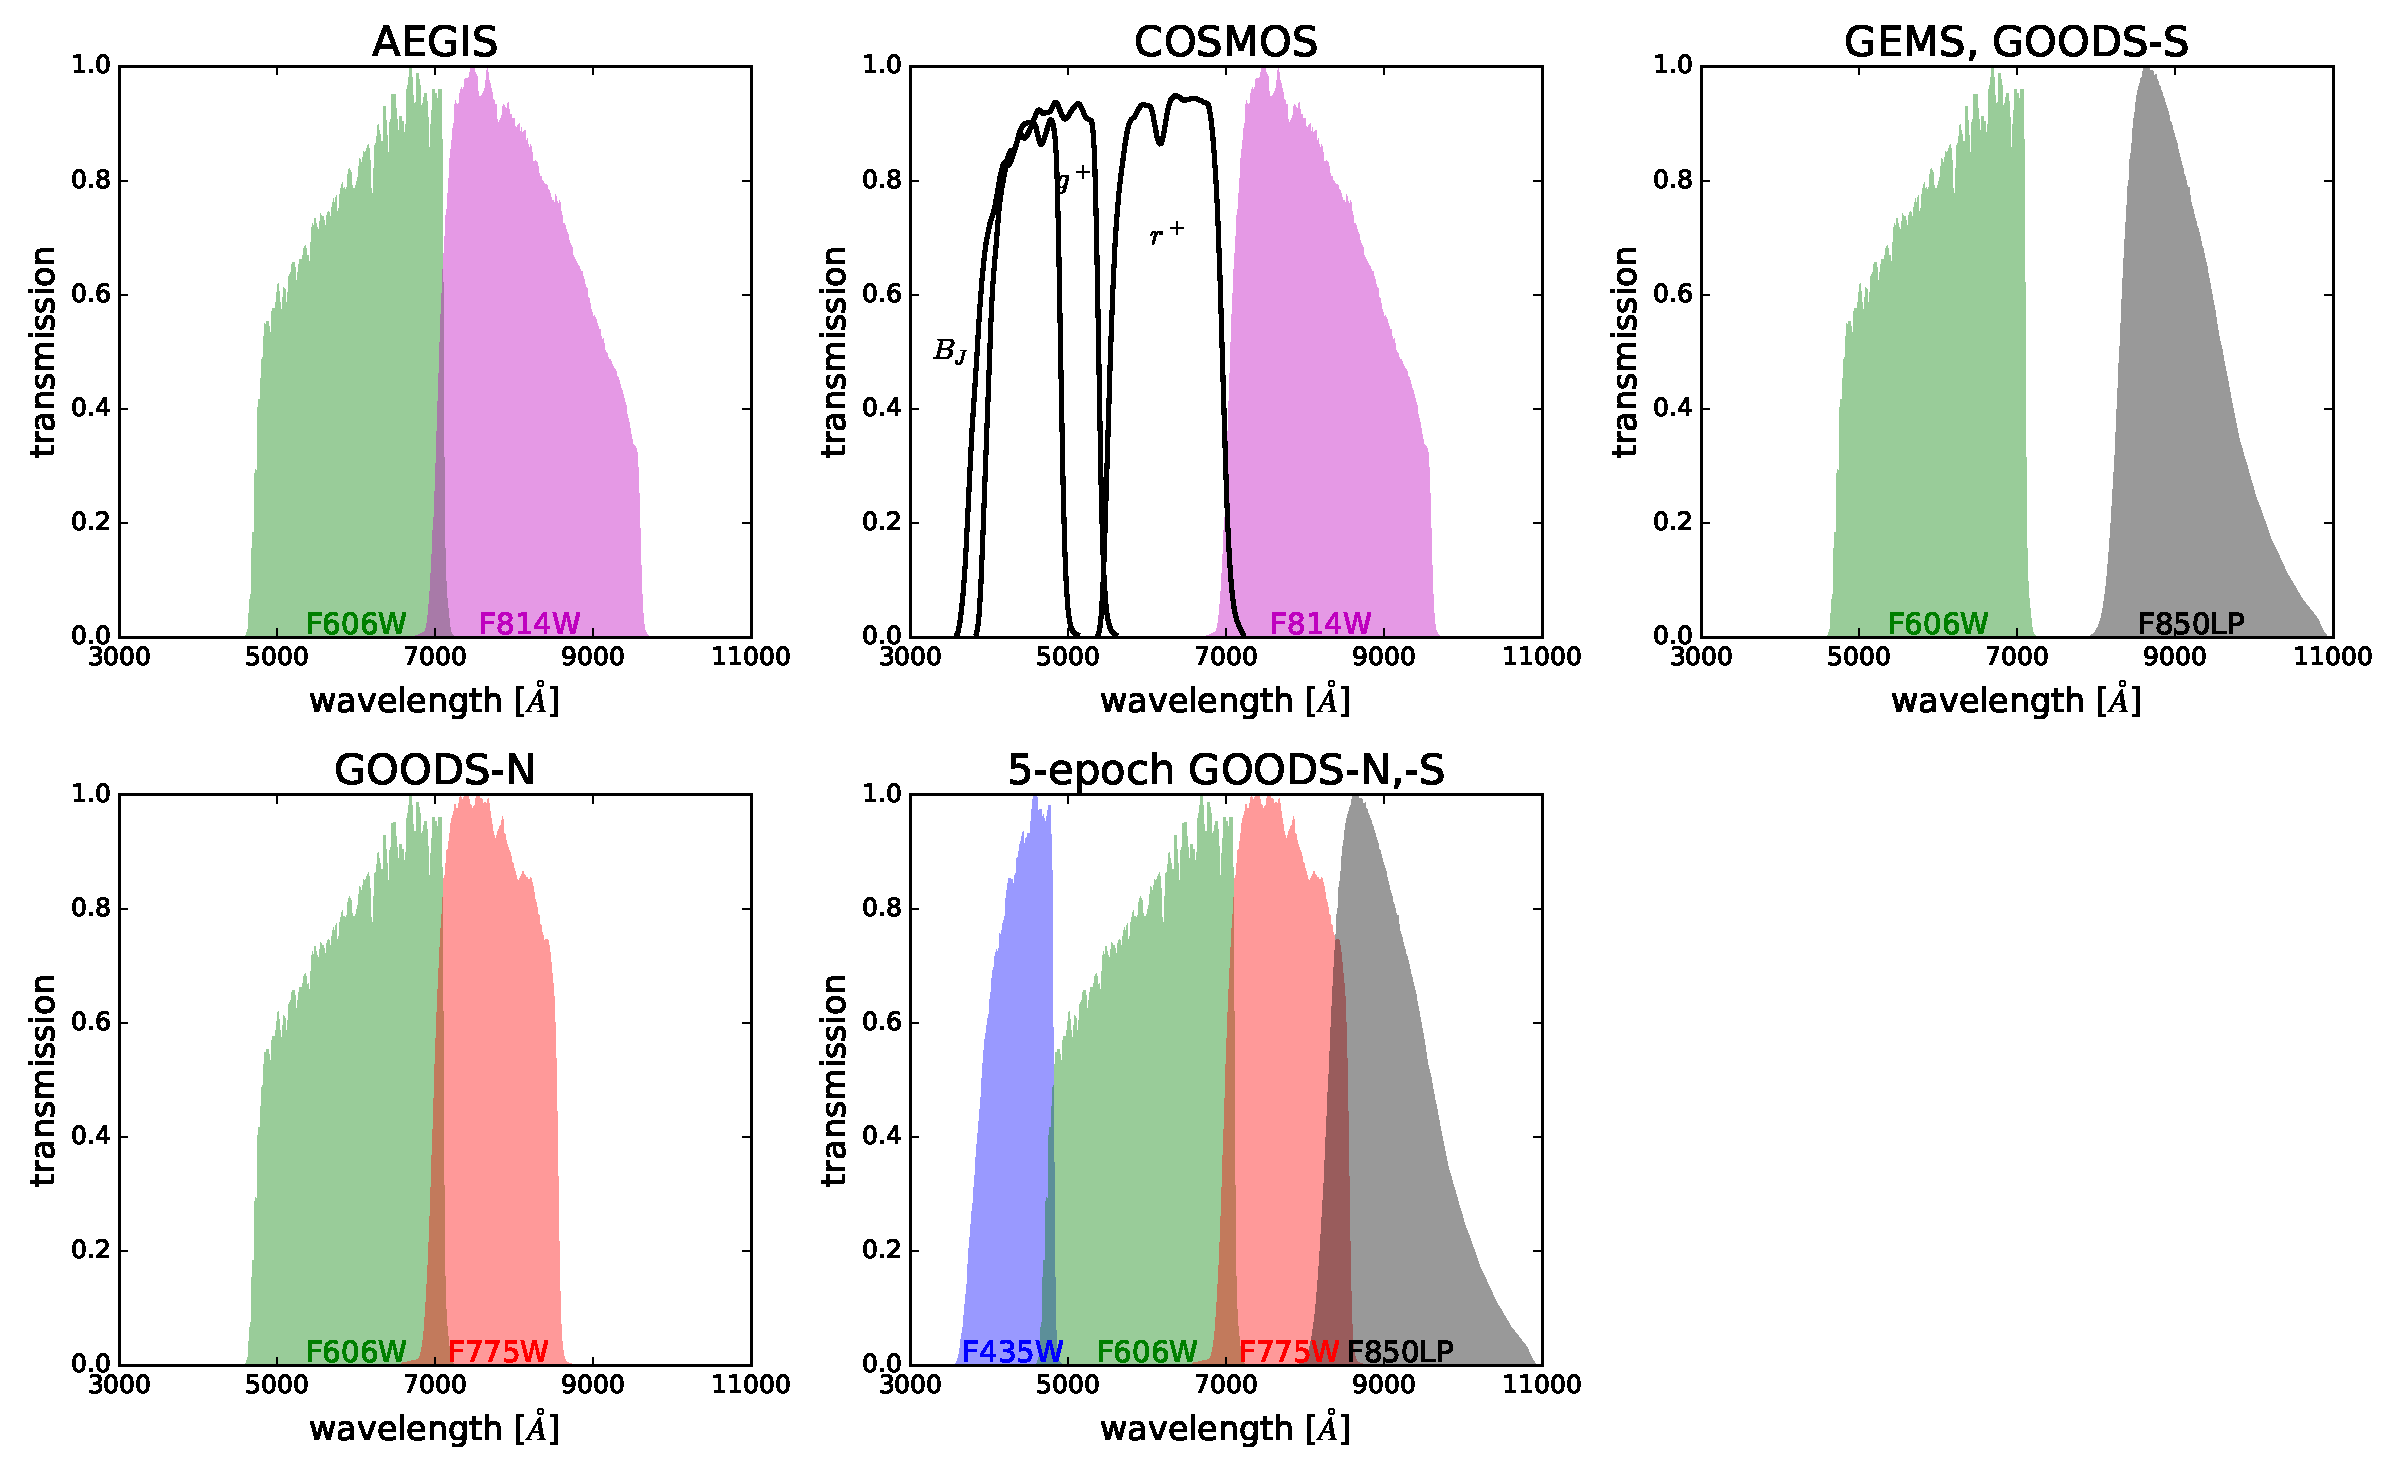
\includegraphics[width=160mm]{figures/filter_curves.pdf}
\caption{Transmission curves of the filters used by \hst{} Advanced Camera for Surveys (ACS) in wide-field channel mode for the various surveys in Galaxy Zoo: Hubble. The unfilled black curves show the filters for the Suprime Camera on the \textit{Subaru} telescope which were used to create color gradients in the composite images for COSMOS.\label{fig:filtercurves}}
\end{figure*}

\subsection{Summary of Hubble Legacy Survey Imaging}\label{ssec:legacy_surveys}

\begin{itemize}
\item \hubble{} ACS imaging for the All-Wavelength Extended Groth Strip International Survey \citep[AEGIS;][]{dav07} covers a strip centered at $\alpha=14^\textrm{h}17^\textrm{m}, \delta=+52^\circ30^\prime$. The strip was originally selected due to low extinction and Galactic/zodiacal emission, making it a prime target for multi-wavelength observations by space-based observatories. The ACS images covered 63 separate tiles over a total area of $\sim710$~arcmin$^2$. Images were in two bands, with exposure times of 2300~seconds in F606W (\Vband) and 2100~seconds in F814W (\Iband). The final mosaic images are dithered to a resolution of 0.03~\arcsec/pixel. For extended objects, the limiting magnitudes of sources in AEGIS are 26.23~(AB) in \Vband{} and 25.61 (AB) in \Iband. 

\item The Great Observatories Origins Deep Survey \citep[GOODS;][]{gia04} covers two well-studied fields in the northern and southern hemispheres: the Hubble Deep Field-North ($\alpha=12^\textrm{h}36^\textrm{m}, \delta=+62^\circ14^\prime$) and the Chandra Deep Field-South ($\alpha=03^\textrm{h}32^\textrm{m}, \delta=-27^\circ48^\prime$). Data including Hubble ACS images are referred to as GOODS-N and GOODS-S, respectively. ACS imaged the GOODS fields in 4 filters -- F435W (\Bband), \Vband, F775W (\iband), and F850LP (\zband). The mean exposure times for each epoch vary by band, from 1050--2100~seconds. The \Bband{} images were completed in a single epoch at the beginning of the survey, but the \Vband, \iband, and \zband{} images were taken in five separate epochs separated by 40--50~days each. The ACS images are dithered to a pixel scale of 0.03~\arcsec/pixel and covers a total area of $\sim320$~arcmin$^2$ (160~arcmin$^2$ per field). The $5\sigma$ limiting magnitudes for extended sources are 25.7 for \Vband{} and 25.0 for \iband. 

\item The Cosmic Evolution Survey \citep[COSMOS;][]{sco07} covers an area of $\sim1.8$~deg$^2$ centered at $\alpha=10^\textrm{h}00^\textrm{m}28^\textrm{s}, \delta=+02^\circ12^\prime21^{\prime\prime}$. Its location near the celestial equator was designed to enable coverage by ground-based telescopes in both the Northern and Southern Hemispheres, as well as the space-based observatories. The \hst{} ACS data from COSMOS consists of 1 orbit with 2028~seconds per pointing in \Iband, consisting of 590 total pointings. The image resolution is dithered to 0.05~\arcsec/pixel. The 50\% completeness magnitude for a galaxy with a half-light radius of $0^{\prime\prime}.50$ in \Iband{} is 24.7 mag. 

\item The Galaxy Evolution from Morphologies and SEDS \citep[GEMS;][]{rix04,cal08} survey is also centered on the Chandra Deep Field-South. The GEMS data covers $\sim800$~arcmin$^2$, and surrounds the area covered by GOODS-S. Images from ACS in GEMS have 1 orbit per pointing for a total of 63~pointings. The exposure times are 2160 and 2286~seconds in \Vband{} and \zband{}, respectively. The image resolution has a pixel scale of 0.03~\arcsec/pixel. The $5\sigma$ limiting magnitudes for source detection are 25.7 AB in \Vband{} and 24.2~AB in \zband. 
\end{itemize}

% Note: galaxy counts remove the duplicate observations from gz_hst_table

\begin{table*}
\center
\caption{Summary of Galaxy Zoo: Hubble imaging \label{tbl:gzh_numbers}}
\begin{tabular}{lclcrr}
\hline\hline
Survey &  $t_{\rm exp}$ & Filters & Resolution & Area & $N_{\rm galaxies}$ \\
 & [sec] & & [\arcsec/pix] & [arcmin$^2$] & \\
\hline
AEGIS                         & 2100$-$2300 & \Vband{} and \Iband{}            & 0.03 & 710   & 8157  \\
COSMOS                        & 2028        & \Iband{}                         & 0.05 & 6480  & 88530 \\
GEMS                          & 2160$-$2286 & \Vband{} and \zband{}            & 0.03 & 800   & 9143  \\
GOODS                         & 1000$-$2100 & \Bband, \Vband, \iband, \zband{} & 0.03 & 320   & 7336  \\
\hspace{10pt} \emph{GOODS-N}  & $-$         & $-$                              & $-$  & $-$   & \emph{2551}  \\
\hspace{10pt} \emph{GOODS-S}  & $-$         & $-$                              & $-$  & $-$   & \emph{4785}  \\
\hline
total                         & $-$         & $-$                              & $-$  & 8310  & 113166  \\
\hline\hline
\end{tabular}
\end{table*}

\subsection{Galaxy selection}

For images from the ACS-GC \citet{gri12}, galaxies are identified using a combination of \sextractor{} \citep{ber96} and the galaxy-profile fitting framework \textsc{Galapagos} \citep{bar12}. We selected all galaxies with $m < 23.5$, where $m$ is in the \Iband, \zband, or \iband{} for the AEGIS + COSMOS, GEMS + GOODS-S, and GOODS-N surveys, respectively. This yielded a total of 113,166~images (Table~\ref{tbl:gzh_numbers}).

Single-epoch images from SDSS Stripe~82 were selected using the same criteria from \citet{wil13}, which required limits of \texttt{petroR90\_r}$ > 3$\arcsec~(where \texttt{petroR90\_r} is the radius containing 90\% of the $r^\prime$ Petrosian flux) and a magnitude brighter than $m_r < 17.77$. 21,522 galaxies in SDSS met these criteria. Coadded images from Stripe~82 were selected from the union of galaxies with coadded magnitudes brighter than $17.77$~mag and the galaxies detected in the single-depth images and matched to a coadd source. This resulted in a larger set of 30,339 images. Of the images in the coadded sample, 5144 (17~percent) are dimmer than the initial magnitude cut of 17.77. 

\subsection{Image creation}

The images used for classification in GZH are color-composite JPGs made from multi-band data. The exact process for creating the images depends on the bands and resolutions in the surveys. 

For galaxies in the ACS General Catalogue \citep[AEGIS, COSMOS, GEMS, 2-epoch GOODS;][]{gri12}, the color composites are made using a fixed pixel intensity scaling with weights of $[2.4\times10^{-4},3\times10^{-4},3\times10^{-4}]$ in the red, green, and blue channels respectively. We also apply a nonlinear mapping to each pixel to emphasize the contrast in faint features \citep{lup04}, taking the form of:

\begin{equation}
I_\mathrm{channel,new} = I_\mathrm{channel,old} \times \frac{\arcsinh(b\times r)}{(b\times r)}
\label{eqn:nonlinear}
\end{equation}

\noindent We adopt a value of $b=3$ for the \hst{} images in \citet{gri12}. 

Since the majority of the data in Legacy surveys described in \S\ref{ssec:legacy_surveys} had images in only 1 or 2~bands available when GZH was launched, making standard 3-channel RGB images in the same method used for the SDSS images in the original Galaxy Zoo was not possible. For surveys with images in two bands (AEGIS, GEMS, and the two-epoch GOODS-N and GOODS-S), the lower-wavelength band is mapped to the blue channel, the higher-wavelength band to the red channel, and the green channel created by taking the geometric mean of the two. Bands used in each of the surveys are listed in Table~\ref{tbl:gzh_numbers}. The 2-epoch GOODS-N and GOODS-S images use different filters --- this was a deliberate choice made so that the GEMS images could be directly compared with the overlapping coverage of GOODS-S (Figure~\ref{fig:filtercurves}). 

By the time that the 5-epoch sets of GOODS data were put into GZH, coverage in four separate \hst{} bands had become publicly available. The deeper GOODS images were created using the arithmetic mean of \Bband{} and \Vband in the blue channel, \Iband{} in the red channel, and \zband in the green channel. These images also had the speckled noise pixels decolorized. 

The COSMOS images only had the \Iband{} imaging available at the time of classification in GZH. For these galaxies, we created ``pseudocolor'' images by using the ACS \Iband{} data as the illumination map and ground-based imaging from the \subaru{} telescope in $B_J$, $r^+$, and $i^+$ filters to provide the color gradients \citep[see][for further details]{gri12}. This means that the images have the angular resolution of \hst{} ($\sim0.05$~\arcsec/pixel) for the overall intensity, but the color gradients are at ground-based resolution, with seeing between 0\arcsec.95 and 1\arcsec.05 \citep{tan07}.

The Stripe~82 single-epoch images were taken directly from the color composites on the DR7 SDSS Skyserver, which combines $g^{\prime}$, $r^{\prime}$, and $i^{\prime}$ exposures into the RGB channels. The coadded Stripe~82 images were assembled from runs 106 and 206 in DR7 and generated as JPGs using the method of \citet{lup04}.

To address a number of images in which the sky noise was highly colored (which might have been a distraction to users), we apply a soft-edged object mask to the image that preserves the color balance for galaxies, but desaturates the speckled noise against regions of blank sky. This technique was applied only to the coadded Stripe~82 and the COSMOS images.

\subsection{Artificial AGN}

We also created a set of images designed to measure the effect of AGN on morphological classifications. Since galactic nuclei can have bright, unresolved optical emission, this has the potential to mimic the effect of a strong bulge. The presence of an AGN is simulated by modeling the PSF for \hst{} and then inserting a bright source near the center of a real galaxy. For each image, the simulated AGN is assigned one of three colors -- either blue, red, or flat (white) as seen in the color images -- and a range of brightnesses such that $L_\mathrm{ratio} \equiv L_\mathrm{galaxy}/L_\mathrm{AGN}$ is in $(0.2,1.0,2.0,5.0,10.0,50.0)$. Combining these parameters generates 15~images with different simulated AGN for each chosen host. 

Two sets of simulated AGN were generated in GZH. The first set (version~1) was assembled from 95~galaxies from GEMS imaging and PSFs from \texttt{daophot}. The second set (version~2) was assembled from 96~galaxies in GOODS-S; this version used deeper imaging and improved PSFs from \texttt{TinyTim}. 

Images with simulated AGN were classified in the main interface in an identical manner and evenly distributed with unaltered images of the galaxies. Classifiers were not explicitly told that the images had been altered, as the goal was to measure the effect on normal classifications in as unbiased a manner as possible. 

\subsection{Galaxy metadata}

Photometric data for the bulk of the GZH sample is largely drawn from the tables provided in \citet{gri12}. This includes photometric parameters from both \sextractor{} and \galfit, such as the fluxes, magnitudes, radii, ellipticities, position angles, and positions. \galfit{} also provides the parametric S\'{e}rsic index and effective half-light radius for the best-fit model. All parameters are measured in both bands of the ACS imaging, with the exception of the single-band COSMOS images.

Redshifts for the GZH catalog are compiled from a variety of sources to include in the GZH catalog. For each galaxy, the redshift selected is in the $\tt Z\_Best$ column of the data (see Table~\ref{tbl:catalog_hst}), its type (spectroscopic: $\tt SPEC\_Z$, photometric: $\tt PHOTO\_Z$, or grism: $ \tt GRISM\_Z$) is listed in the column $\tt Z\_BEST\_TYPE$, and the source catalog ($\tt ACSGC$ \citep{gri12}, $\tt 3DHST$ \citep{mom15}, $\tt MUSYC$ \citep{car10}, or $\tt UltraVISTA$ \citep{ilb13}) of the redshift is in column $\tt Z\_BEST\_SOURCE$.

For galaxies which have redshifts from multiple sources, we use the following algorithm to select the $\tt Z\_BEST$ redshift. We first prioritize spectroscopic redshifts; these are provided in the ACS-GC, 3DHST, and MUSYC catalogs. If a high quality spec-z exists in the ACS-GC. we use that, else 3DHST, else MUSYC. More 98\% of the matched spec-$z$'s are consistent at $\Delta z<0.001$; therefore, the priority order of selection makes no negligible difference in this sample. If no spectroscipic redshifts are available, we compare the 1-$\sigma$ errors of the photometric (ACS-GC, 3DHST, MUSYC, UltraVISTA) and grism (UltraVISTA) redshifts, and use the redshift with the smallest error. Table~\ref{tbl:redshifts} shows the results of this selection. 
 
%\begin{figure*}
%\center
%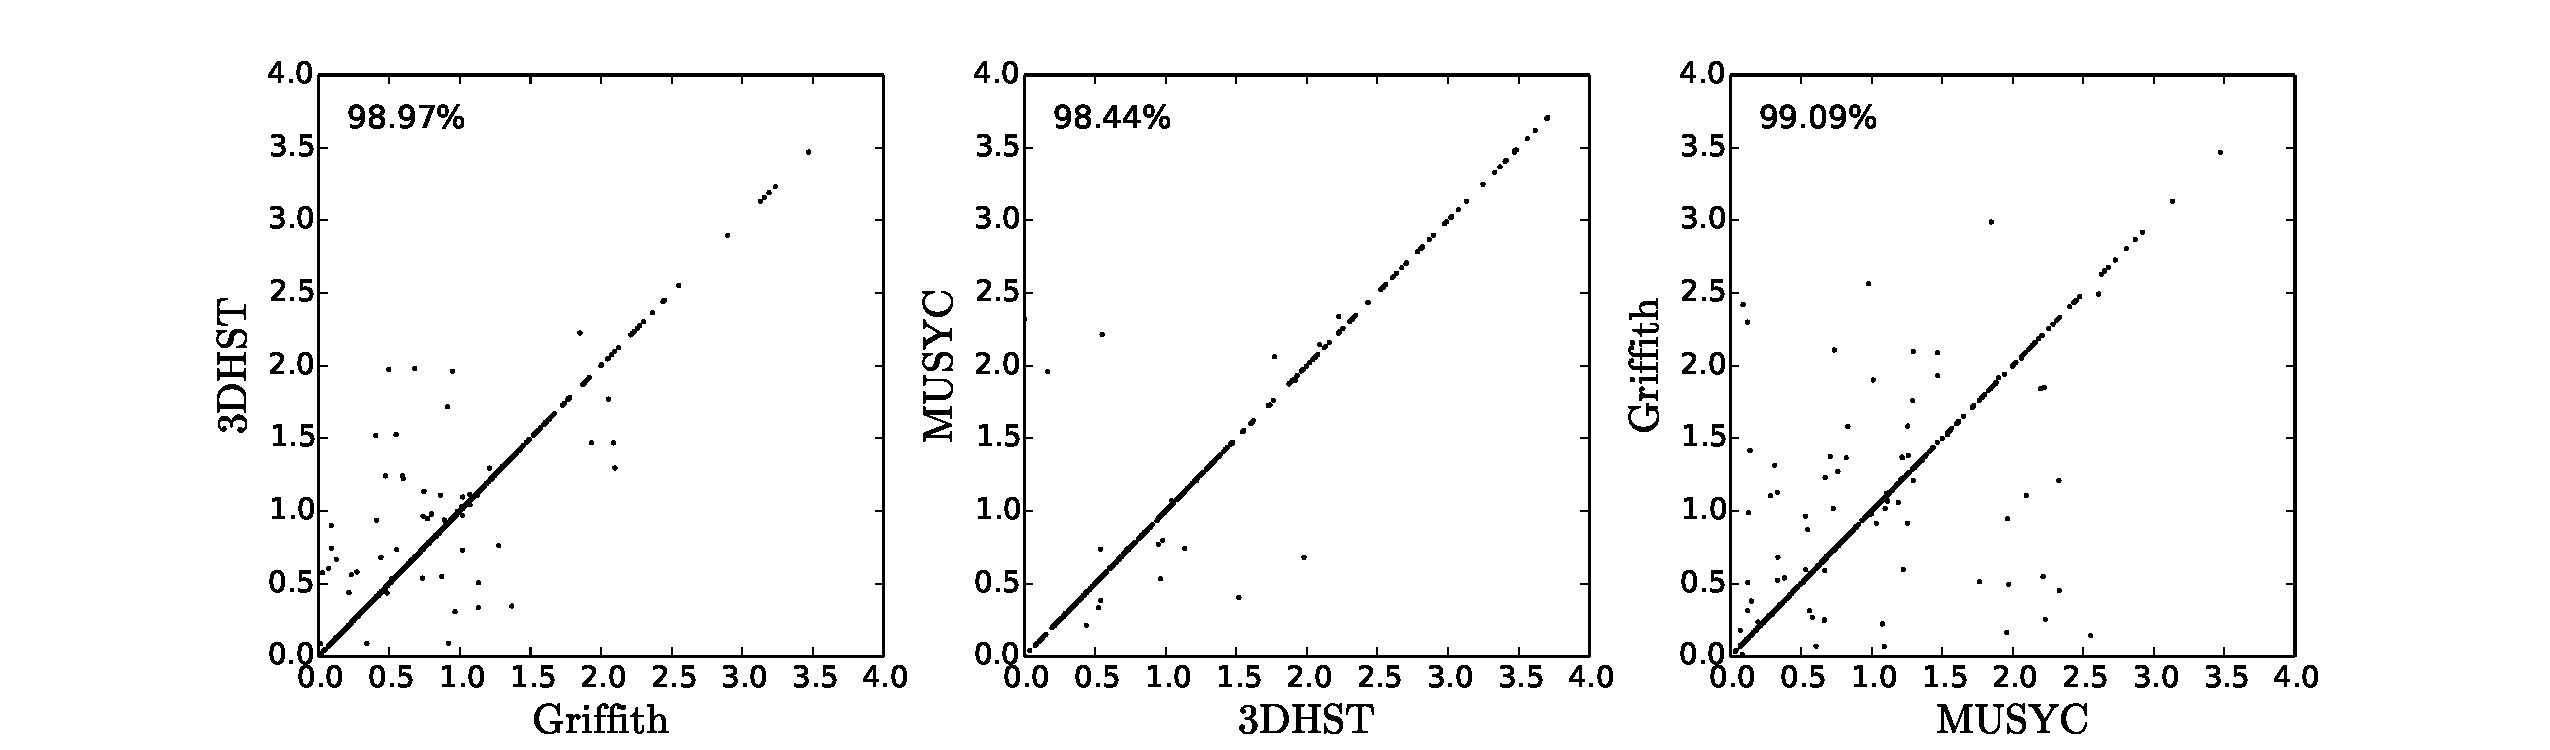
\includegraphics[width=160mm]{figures/specz_comparison.pdf}
%\caption{Spectroscopic redshifts from the ACS-GC, 3DHST, and MUSYC catalogs. The number in the upper left of each plot is the percentage of redshifts which agree within $\Delta z < 0.05$ between the two catalogs being compared in each panel. Within this range there is over 98\% agreement in redshifts between all three catalogs.}
%\label{fig:speczs}
%\end{figure*}


\tabletypesize{\scriptsize}
\begin{deluxetable*}{l|rr|rrr|rr|r|rr}
\tablecolumns{12}
\tablewidth{0pc}
\tablecaption{GZH redshifts by survey\label{tbl:redshifts}} 
\tabletypesize{\scriptsize}
\tablehead{
 &   
\multicolumn{2}{c}{\underline{ACS-GC}} &
\multicolumn{3}{c}{\underline{3DHST}} &
\multicolumn{2}{c}{\underline{MUSYC}} &
\multicolumn{1}{c}{\underline{UltraVISTA}}&
\multicolumn{2}{c}{\underline{Total}} 
\\
\colhead{Survey} & 
\colhead{spec-z} & 
\colhead{photo-z} & 
\colhead{spec-z} & 
\colhead{grism-z} & 
\colhead{photo-z} & 
\colhead{spec-z} & 
\colhead{photo-z} & 
\colhead{photo-z} & 
\colhead{with redshift} &
\colhead{in survey}
}
\small
\startdata
%Survey     Gs        Gp    3ds    3dg     3dp       Ms      Mp       UVp       total
AEGIS    & 3,656  & 2,941  & 12  &  515  &  249    & 0     & 0     &  0      & 7,373  & 8,507\\
COSMOS   & 7,201  & 77,435 & 35  &  358  &  26     & 0     & 0     &  2,665  & 85,020 & 92,808 \\
GEMS     & 387    & 628    & 6   &  99   &  40     & 279   & 7,304 & 0       & 8,743  & 9,304\\
GOODS-N  & 1,947  & 37     & 418 & 1,545 &  1,381  & 0     & 0     & 0       & 5,328  & 12,030 \\
GOODS-S  & 1,080  & 4      & 327 & 1,348 &  281    & 816   & 1,184 & 0       & 5,040  & 10,284 \\
SDSS     & 0      & 0      & 0   &  0    &  0      & 0     & 0     & 0       & 37,545 & 51,861  \\
\hline
Total    & 14,271 & 81,045 & 798 & 3,865 & 1,977   & 1,095 & 8,488 & 2,665   & 114,204 & 184,794\\
\enddata
\end{deluxetable*}

Photometric and spectroscopic data for the SDSS Stripe~82 galaxies are taken from the CasJobs DR7 tables. This includes $ugriz$ Petrosian magnitudes and fluxes, as well as the relative de~Vaucouleurs and exponential fits from the model magnitudes. Redshifts used for the Sloan galaxies are all spectroscopic. 82.6\% of galaxies in the single-depth images and 65.1\% of galaxies in the coadd images have a measured DR7 spectroscopic redshift. 


\section{Galaxy Zoo interface and classifications}\label{sec:interface}

\begin{figure*}
\center
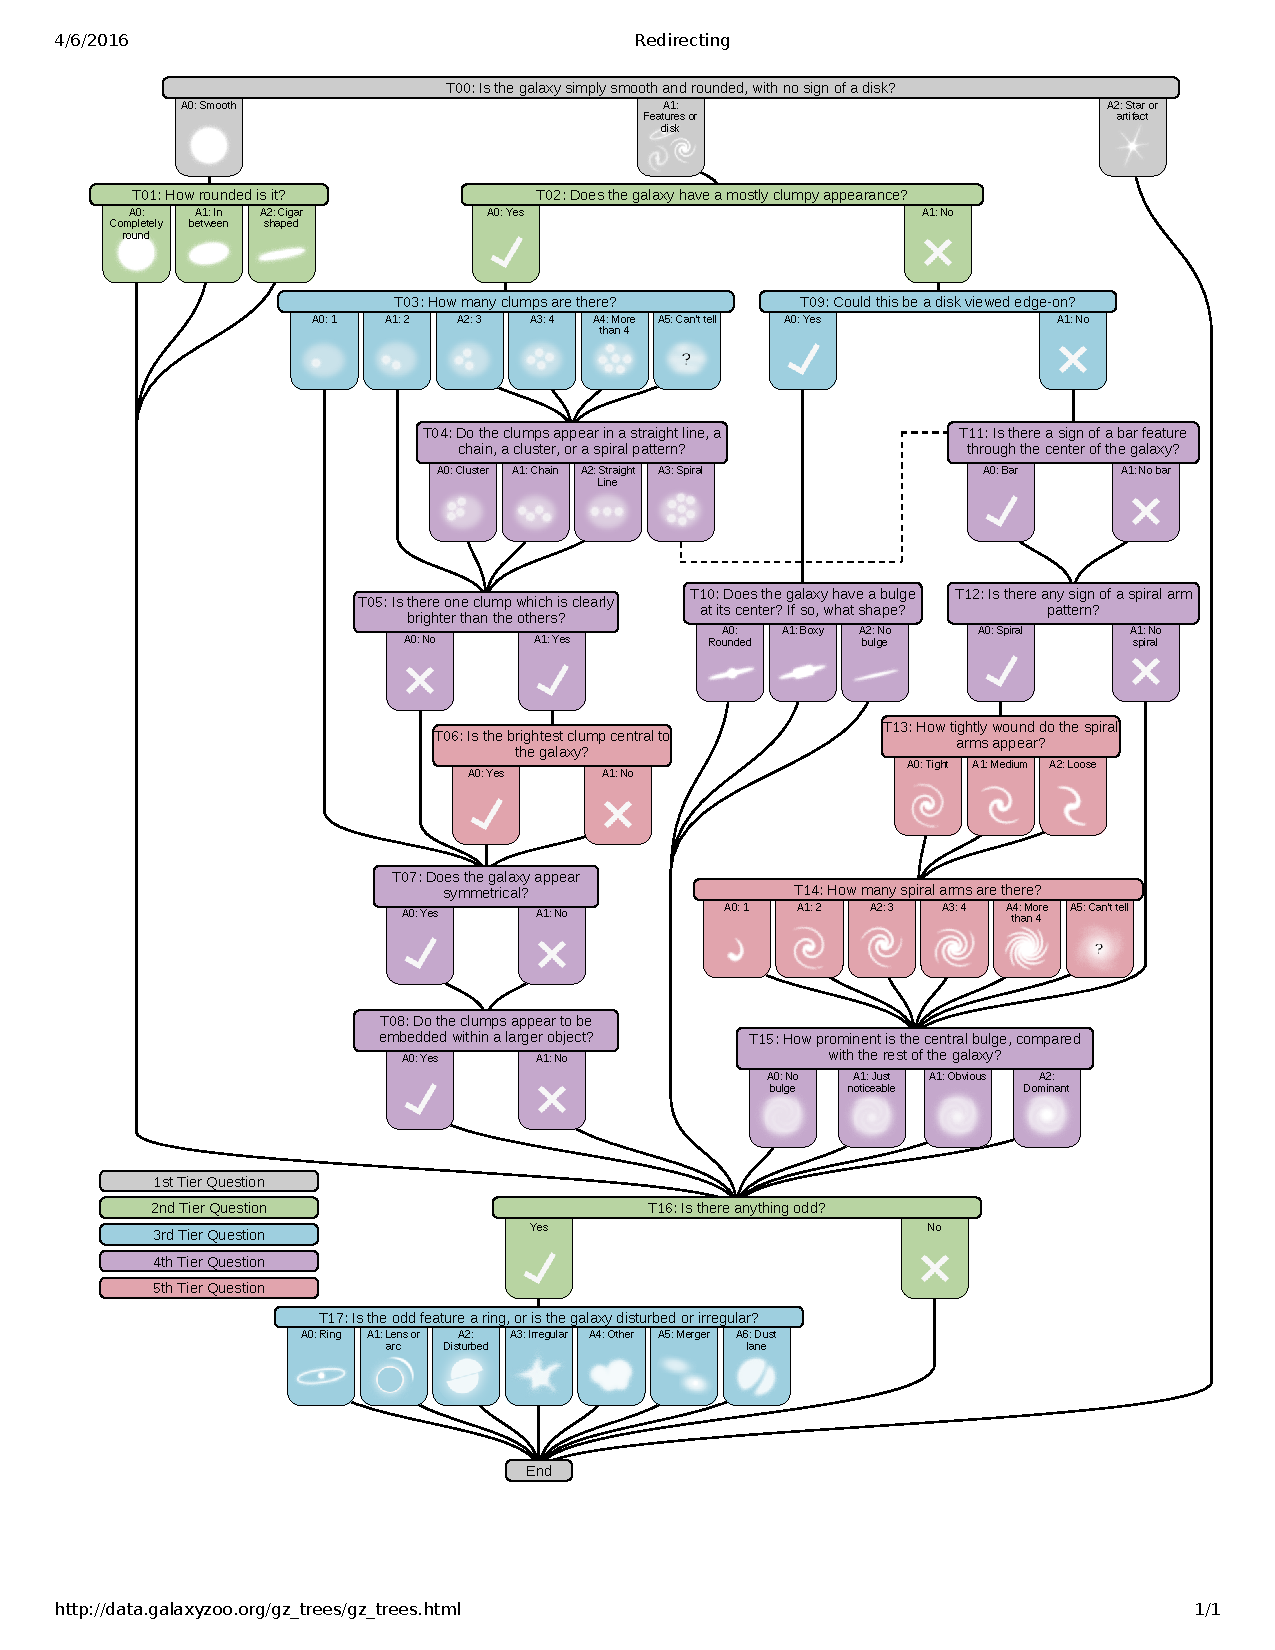
\includegraphics[width=\textwidth]{figures/gzh_decision_tree.pdf}
\caption{Flowchart of the questions presented to GZH users, labeled with the corresponding Task numbers. Tasks in the decision tree are color-coded by tier level: Gray-colored Tasks are 1st tier questions which are asked of all users. Tasks colored green, blue, purple, and pink (respectively) are one, two, three, or four steps below branching points in the decision tree.}
\label{fig:decisiontree}
\end{figure*}


\subsection{User weighting}\label{ssec:weighting}
The votes of individual users who classified galaxies in GZH are combined to make a vote fraction for each question on the classification tree. Users' votes are weighted slightly \citep[in a method identical to that described in][]{wil13} such that users who frequently disagree with all other users end up having very low weights. The user weighting $w$ is 1 for the top 95\% of users as ranked by consistency. For the bottom 5\% of users, $w$ drops smoothly and is effectively zero for only the bottom 1\% of classifiers in the CDF. The overall effect on the GZH dataset is relatively small, but this method is effective at filtering out contributions from random or delibrately malicious classifiers.

\subsection{Interface and decision tree}\label{ssec:interface}

\begin{figure*}
\center
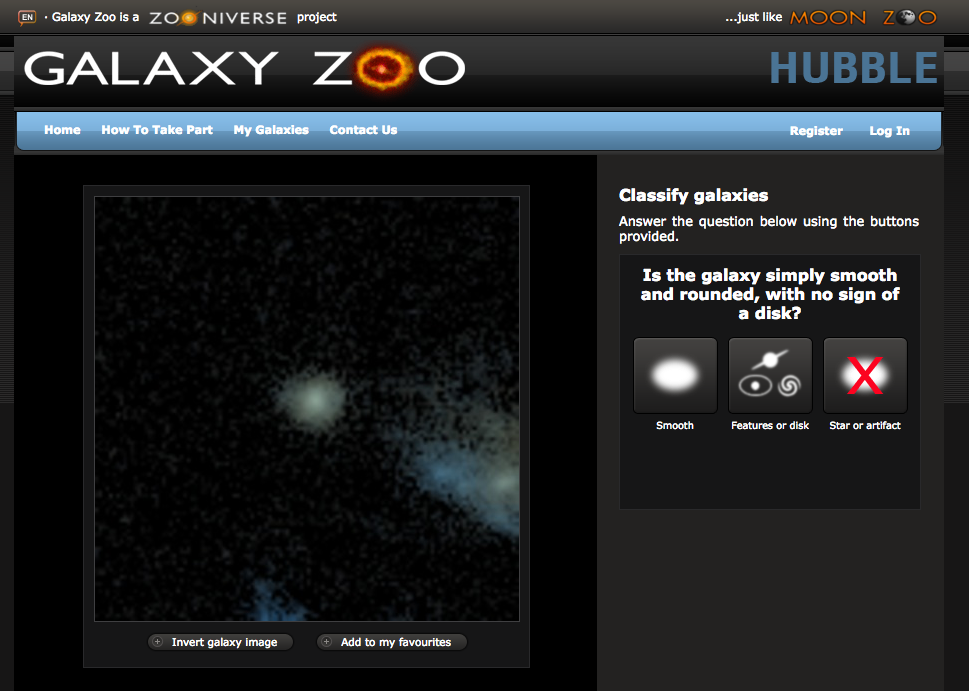
\includegraphics[width=160mm]{figures/gzh_interface.png}
\caption{Screenshot of the Galaxy Zoo: Hubble interface at the beginning of a classification, with the user ready to select an answer for the first question in the decision tree.\label{fig:interface}}
\end{figure*}


\section{Correcting for redshift-dependent classification bias}\label{sec:debiasing}

The previous versions of Galaxy Zoo morphology classifications \citep{lin08,wil13} were based on observations of galaxies in the Sloan Digital Sky Survey (SDSS) which have a median redshift of $z<0.2$. In these cases, it was assumed that there was no cosmological evolution of the morphologies of galaxies and therefore any observed changes in the distribution of galaxies with different consensus morphologies was due to the effects of redshift on the image quality (\ie. the reduction in physical resolution, surface brightness dimming, etc). For both previous releases of GZ morphologies, we provided a correction for redshift-dependent bias based on matching the classification fractions at the highest redshfts with those at the lowest redshift. See \citet{bam09} and \citet{wil13} for the details. 

In the GZH samples, the redshift range is large enough that we expect to measure cosmological evolution of the types and morphologies of galaxies in the sample. As a result, the previous methods of correcting for redshift dependent bias will not work. In addition, the effects of band shifting will change the images even more across these redshift ranges. %Figure~\ref{fig:exampleFERENGI} illustrates some of the possible effects of losing features in spiral galaxies at high redshift. 

In order to test and correct for the effects of redshift, we generated a set of calibration images. These images consist of the same galaxy as it would appear over a variety of redshifts. The input images are from the SDSS \citep{yor00,str02} and are processed using the \ferengi{} code \citep{bar08a} to match the observational properties of the \hst{} surveys out to $z=1$. These images were classified in the Galaxy Zoo interface using the same classification scheme as the original \hst{} images.
 
\subsection{Selection of FERENGI input galaxies}

We selected 288 unique galaxies from SDSS imaging to run through the \ferengi{} code. The selection spanned a variety of galaxy morphologies (as selected by GZ2 classifications) and $r^\prime$-band surface brightnesses, and also spanned the redshift range of SDSS targets (in $N_z = 4$ bins) in order to be optimized for different target minimum redshifts in \hst{} imaging. 

%The selection criteria for the different morphological categories is summarized in Table \ref{tbl:morphologies}. 
The surface brightness selection ($N_\mu = 3$) for the FERENGI galaxies was (1) low: $\mu > 21.5$~\magarc;  (2) mid: $20.5 < \mu < 21.5$~\magarc; and (3) high: $\mu < 20.5$~\magarc. For each of the four ``target redshifts'' ($z = 0.3, 0.5, 0.8$ and $1.0$), the images were redshifted in $\Delta z = 0.1$ bins up to $z=1.0$. 
 
%\begin{table*}
%\center
%\caption{Summary of morphological categories selected for FERENGI sample.\label{tbl:morphologies}}
%\begin{tabular}{lllc}
%\hline\hline
%Morphology          & Label &  Selection                                                                                            & $N_{\rm objects}$ \\
%                    &       &                                                                                                       & [$N_z \times N_\mu$] \\
%\hline
%Features            & Yes       & $p_{\rm features} > 0.8$, $p_{\rm odd} < 0.1$                                                         & 12 \\ 
%                    & Int.      & $0.3 < p_{\rm smooth} < 0.6$, $p_{\rm odd} < 0.1$                                                     & 12 \\ 
%                    & No        & $p_{\rm smooth} > 0.8$, $p_{\rm odd} < 0.1$                                                           & 12 \\ 
%Merger              & No        & $p_{\rm features} > 0.8$, $p_{\rm odd < 0.1}$, $p_{\rm merger} < 0.1$                                 & 12 \\
%                    & Int.      & $p_{\rm odd} > 0.5$, $0.1< p_{\rm merger} < 0.4$                                                      & 12 \\ 
%                    & Yes       & $p_{\rm odd} > 0.5$, $p_{\rm merger} > 0.4$                                                           & 12 \\
%Edge-on             & Yes       & $p_{\rm edgeon} > 0.8$, $p_{\rm features} > 0.5$                                                      & 12 \\
%                    & Int.      & $0.4 < p_{\rm edgeon} < 0.8$ , $p_{\rm features} > 0.5$                                               & 12 \\
%                    & No        & $p_{\rm edgeon} < 0.2$, $p_{\rm features} > 0.5$                                                      & 12 \\
%Bar                 & No        & $p_{\rm bar} < 0.1$, $p_{\rm features} > 0.5$, $p_{\rm edgeon} < 0.2$                                 & 24 \\
%                    & Int.      & $0.2 < p_{\rm bar} < 0.4$, $p_{\rm features} > 0.5$, $p_{\rm edgeon} < 0.2$                           & 24 \\
%                    & Yes       & $p_{\rm bar} > 0.8$, $p_{\rm features} > 0.5$, $p_{\rm edgeon} < 0.2$                                 & 24 \\
%Visible spiral      & No        & $p_{\rm spiral} < 0.2$, $p_{\rm features} > 0.5$, $p_{\rm edgeon} < 0.2$, $p_{\rm bar} < 0.1$         & 12 \\
%                    & Int.      & $0.2 < p_{\rm spiral} < 0.8$, $p_{\rm features} > 0.5$, $p_{\rm edgeon} < 0.2$, $p_{\rm bar} < 0.1$   & 12 \\
%                    & Yes       & $p_{\rm spiral} > 0.8$, $p_{\rm features} > 0.5$, $p_{\rm edgeon} < 0.2$, $p_{\rm bar} < 0.1$         & 12 \\
%Oblique bulge size  & No        & $p_{\rm nobulge>0.6}$, $p_{\rm features} > 0.5$, $p_{\rm edgeon} < 0.5$, $p_{\rm bar} < 0.2$          & 12 \\
%                    & Int.      & $p_{\rm justnoticeable}>0.6$, $p_{\rm features} > 0.5$, $p_{\rm edgeon} < 0.5$, $p_{\rm bar} < 0.2$   & 12 \\
%                    & Yes       & $p_{\rm obvious|dominant}>0.5$, $p_{\rm features} > 0.5$, $p_{\rm edgeon} < 0.5$, $p_{\rm bar} < 0.2$ & 12 \\
%Edge-on bulge shape & Round     & $p_{\rm rounded}>0.5$, $p_{\rm features} > 0.5$, $p_{\rm edgeon} > 0.5$                               & 12 \\
%                    & Boxy      & $p_{\rm boxy}>0.4$, $p_{\rm features} > 0.5$, $p_{\rm edgeon} > 0.2$                                  & 12 \\
%                    & No bulge  & $p_{\rm nobulge}>0.5$, $p_{\rm features} > 0.5$, $p_{\rm edgeon} > 0.5$                               & 12 \\
%\hline\hline
%\end{tabular}
%\end{table*}

In addition to the physical parameters of the input images, the \ferengi{} output depends on assumptions of the global galaxy evolution model. This evolution is a crude mechanism that mimics the brightness increase of galaxies with increasing redshift (out to at least $z\sim1-2$). The effect on the redshifted images is simply an empirical addition to the magnitude of a galaxy of the form $M' = e\times z + M$, where $M'$ is the corrected magnitude, and $e$ is the evolutionary correction in magnitudes (i.e., $e=-1$ essentially brightens the galaxy by 1~magnitude by $z=1$). We ran \ferengi{} for values of $e$ starting from $e=0$ and decreasing to $e=-3.5$ in increments of $\Delta e = 0.5$. Figure~\ref{fig:exampleFERENGI} shows several examples of the effects of ``losing`` spiral/disc features with increasing redshift for two galaxies with $e=0$. 

The final number of \ferengi{} images produced for each galaxy is ultimately a function of galaxy's redshift, since the new images cannot be resampled at better angular resolution than the original SDSS data, as well as the number of $e$ values selected. Table~\ref{tbl:ferengivalues} summarizes the total sample of redshifted images produced for GZH. 

\begin{table}
\caption{Summary of FERENGI artificial redshifting \label{tbl:ferengivalues}}
\begin{tabular}{lccccr}
\hline\hline
$z_{\rm target}$ & $N_{z {\rm bins}}$ & $N_{\rm evolution}$ & $e_{\rm max}$ & $N_{\rm galaxies}$ & $N_{\rm images}$\\
\hline
0.3              & 8                  & 7                   & $-3.0$        & 72             & 4032 \\
0.5              & 6                  & 4                   & $-1.5$        & 72             & 1728 \\
0.8              & 3                  & 3                   & $-1.0$        & 72             &  648 \\
1.0              & 1                  & 3                   & $-1.0$        & 72             &  216 \\
\hline\hline
\end{tabular}
\end{table}

\begin{figure*}
\center
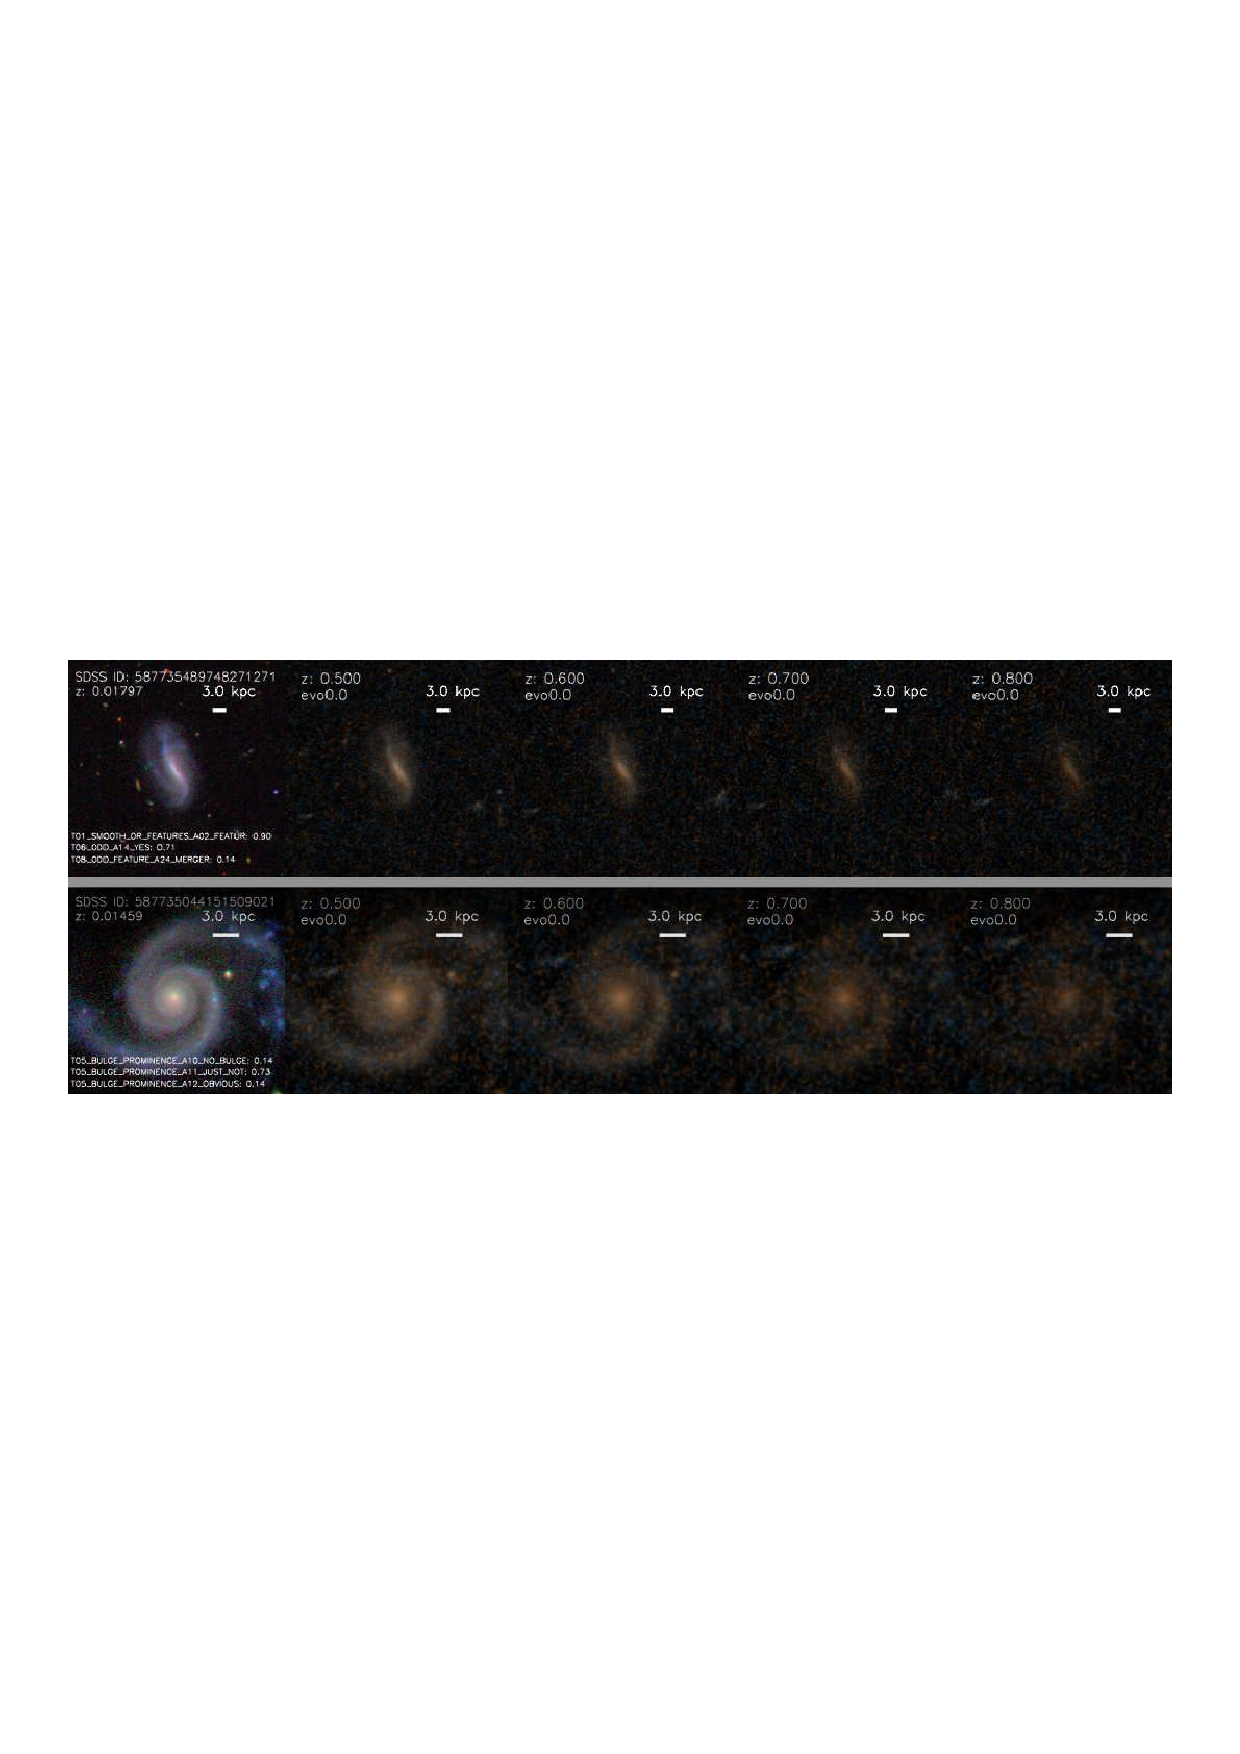
\includegraphics[width=160mm]{figures/example_ferengi.pdf}
\caption{Examples of two galaxies which have been run through the FERENGI code to produce simulated \hst{} images. The measured value of \pfeatures{} from GZH for the images in each panel are (1) Top row: \pfeatures~= (0.900, 0.625, 0.350, 0.350, 0.225) and (2) Bottom row: \pfeatures~= (1.000, 0.875, 0.875, 0.625, 0.375). \label{fig:exampleFERENGI}}
\end{figure*}

\subsection{Correcting GZH morphologies for classification bias}\label{ssec:zeta}

The approach used in GZH for correcting the weighted classifications for user bias rests on the assumption that the \emph{amount} of bias is a function of the apparent size and brightness of the image as seen on screen. This is controlled by two types of parameters: \textbf{intrinsic} properties of the galaxy itself, such as its physical diameter and luminosity, and \textbf{extrinsic} properties, such as the distance (redshift) of the galaxy and its relative orientation. There are likely other parameters that affect user accuracy, such as the proximity of close companions \citep[``distraction bias''; see][]{joh15} or bias as a function of the individual user. The combination of all such parameters forms a high-dimensional space, and we have insufficient data to measure their individual effects. Instead, we use just two parameters that are intended to capture the bulk of the change in bias (based on GZ1/GZ2): a galaxy's $r^\prime$-band surface brightness ($\mu_r$; intrinsic) and redshift ($z$; extrinsic). 

The change in bias as a function of $\mu_r$ and $z$ is measured using the \ferengi{} images over all the evolutionary correction factors. We assume that the ``true'' (ie, debiased) vote fraction $f_{\mu,z}$ for a galaxy can be expressed as:

\begin{equation}
f_{\mu,z} = \left(f_{\mu,z=0.3}\right) \times e^{{\frac{z-z_0}{\zeta}}},
\label{eqn:fzeta}
\end{equation}

\noindent where $f_{\mu,z=0.3}$ is the ``calibrated'' vote fraction at the lowest redshift in the \ferengi{} bins ($z=0.3$) and $\zeta$ is a positive parameter that controls the rate at which $f$ decreases with increasing redshift. This formula fits the data relatively well (with almost no exceptions, the vote fractions for featured galaxies decrease monotonically with increasing redshift), and the exponential function bounds the observed vote fractions between $f_{\mu,z=0.3}$ and zero. Figure~\ref{fig:zeta_examples} show examples of the change in vote fraction and their fits to Equation~\ref{eqn:fzeta} for a random selection of galaxies in the \ferengi{} images. 

\begin{figure*}
\center
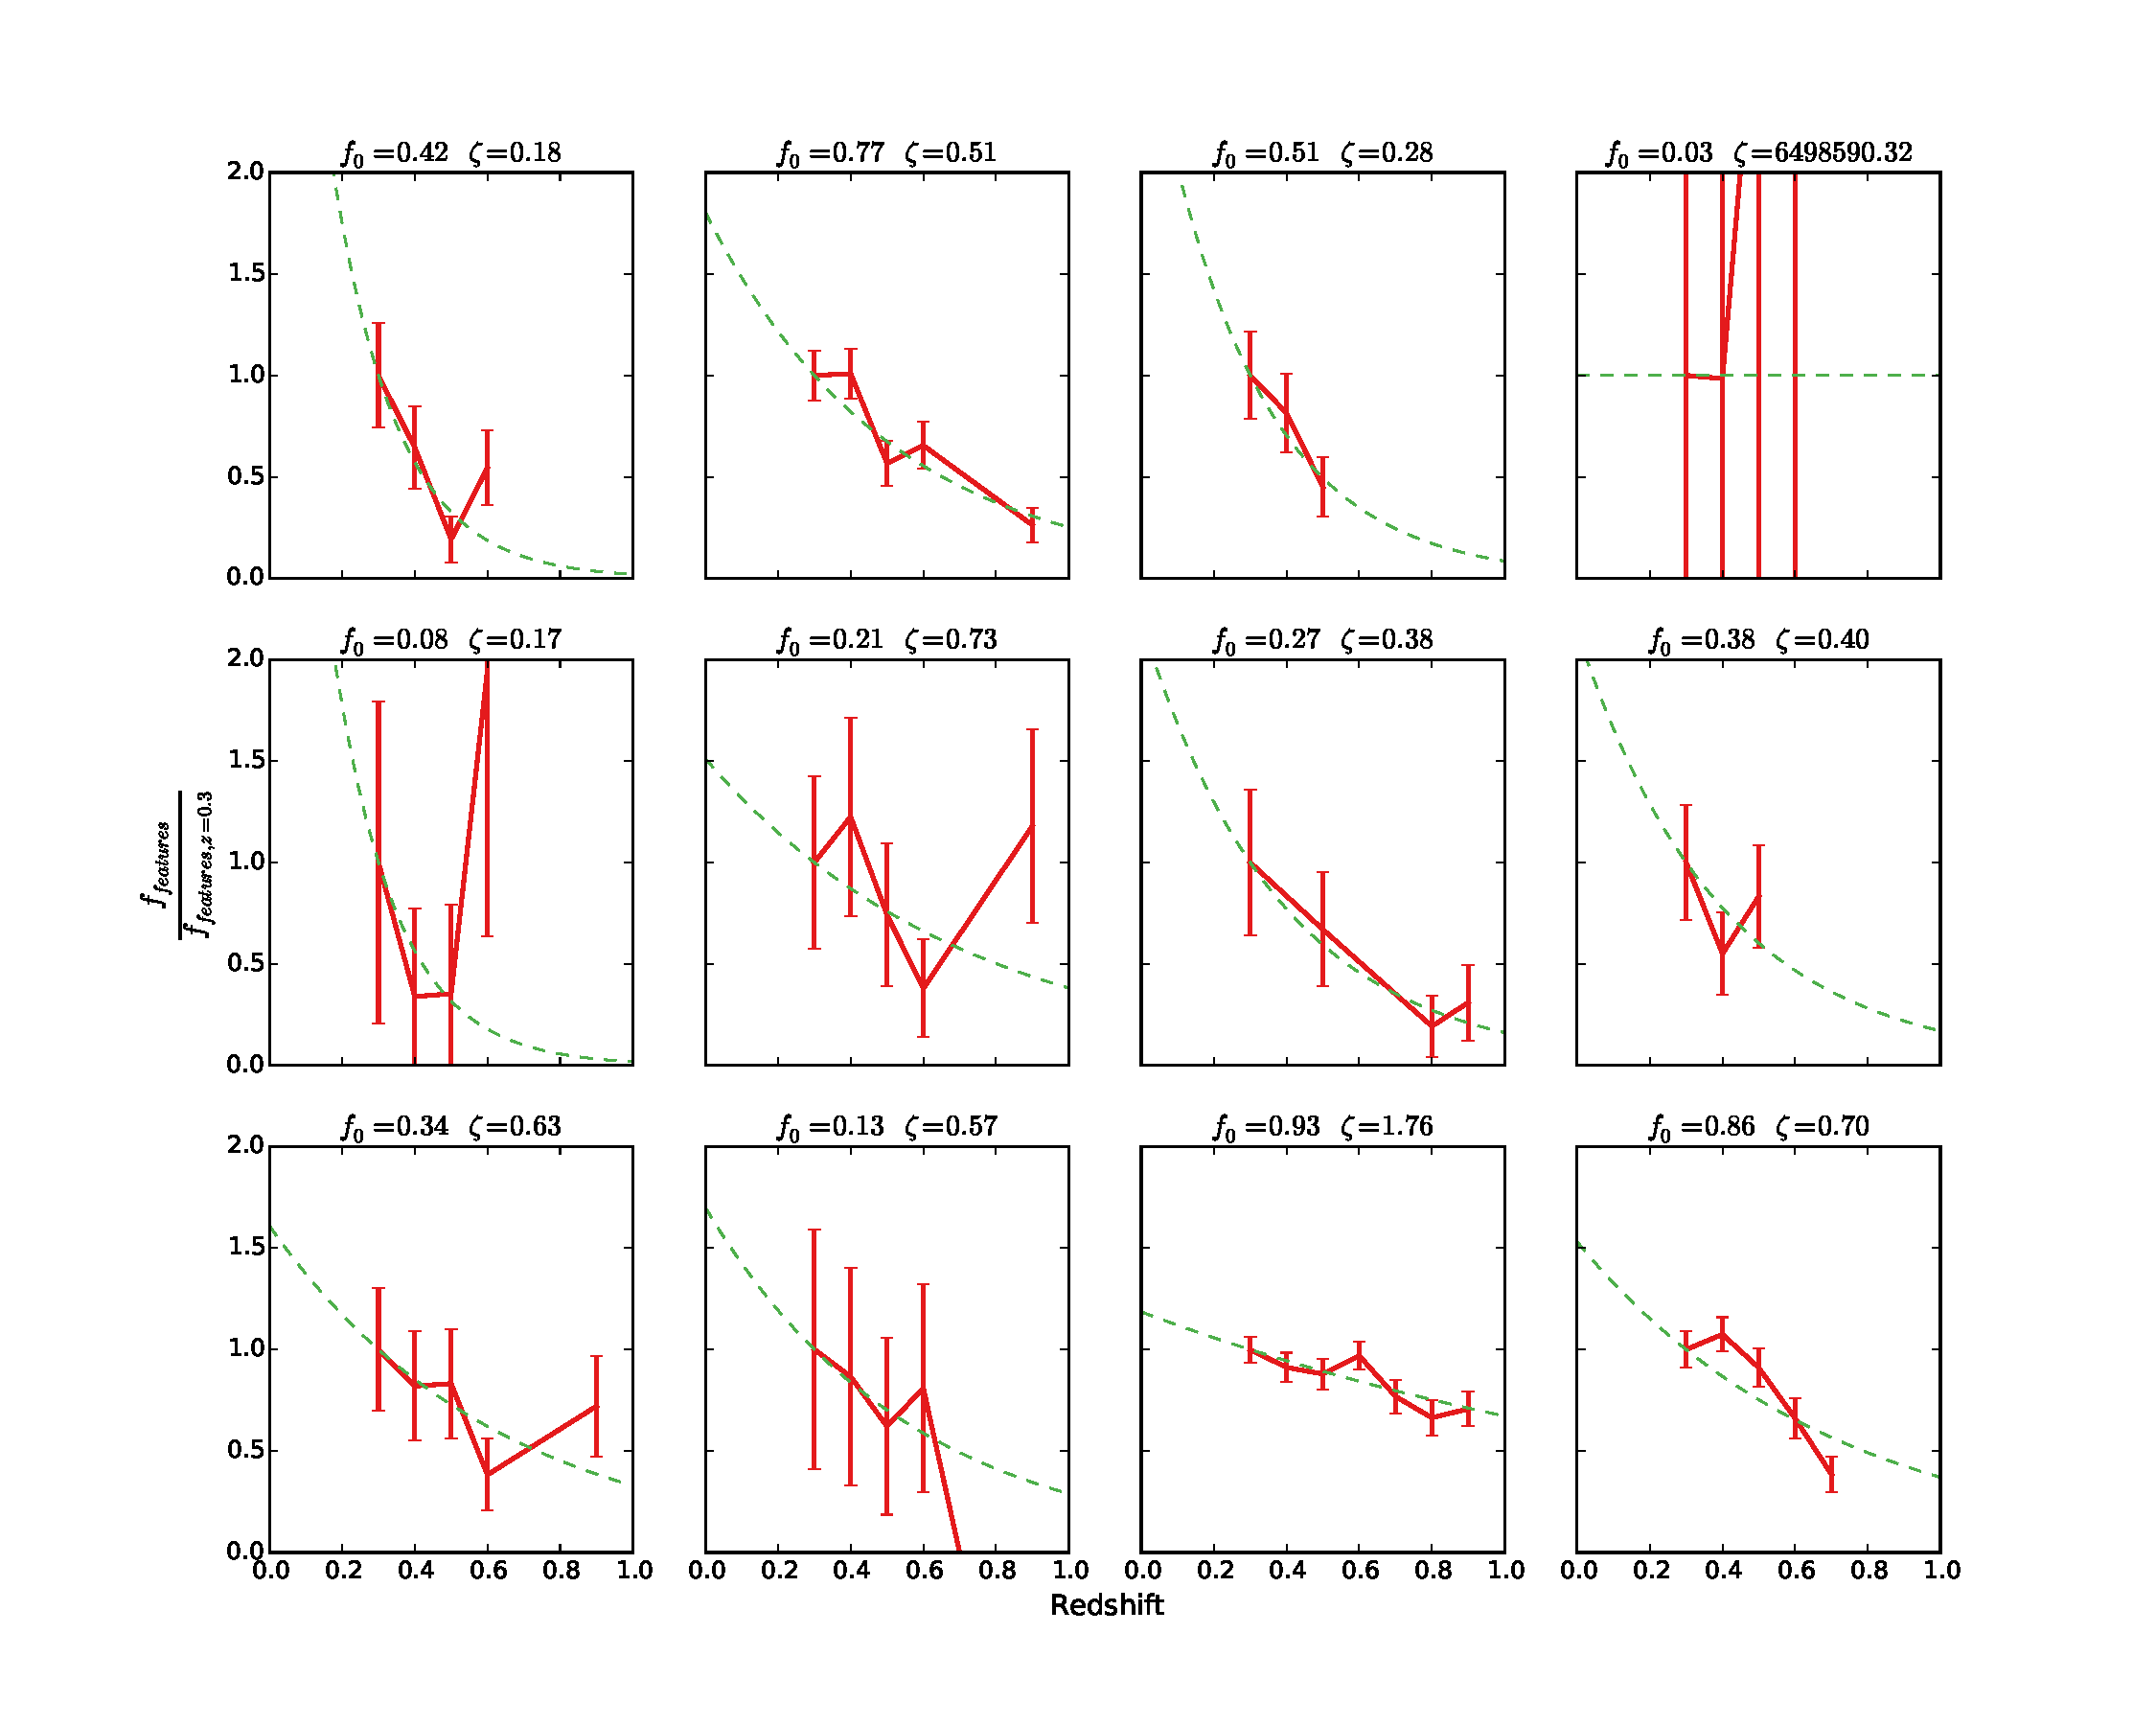
\includegraphics[width=\textwidth]{figures/zeta_examples.pdf}
\caption{Behavior of the normalized, weighted vote fractions of features visible in a galaxy ($f_\textrm{features}$) as a function of redshift in the artifical \ferengi{} images. Galaxies in this plot were randomly selected from a distribution with $e=0$ and at least three detectable images in redshift bins of $z\ge0.3$. Measured vote fractions (red points) are fit with an exponential function (Equation~\ref{eqn:fzeta}); the best-fit parameters are given above each plot. Error bars are Poissonian, assuming a median of 40~votes per galaxy.}
\label{fig:zeta_examples}
\end{figure*}

We use the values of $\zeta$ for \emph{all} sets of artifically redshifted galaxies to fit the overall distribution as a function of surface brightness, since we expect the correction being applied to vary as a function of the intrinsic galaxy properties. We restrict the galaxies that can be used to measure the calibration to those with data at the pivot redshift of $z=0.3$, non-zero $f_\textrm{features}$ at $z=0.3$, and with a reasonable fit to the exponential model ($\Delta \chi^2 > 3.0$). 

Figure~\ref{fig:zeta_mu} shows the results of fitting the \ferengi{} images with Equation~\ref{eqn:fzeta}; the correction is a weak function of galaxy surface brightness. Higher-surface brightness galaxies have stronger average corrections, likely because these galaxies are more likely to have larger $f_\textrm{features}$ values at high redshifts. Low surface brightness galaxies are more likely to begin low and remain low; the bounded nature of the dropoff (and Poissonian-like variance among the individual voters) means that the average magnitude of $\zeta$ will be less. 

\begin{figure}
\center
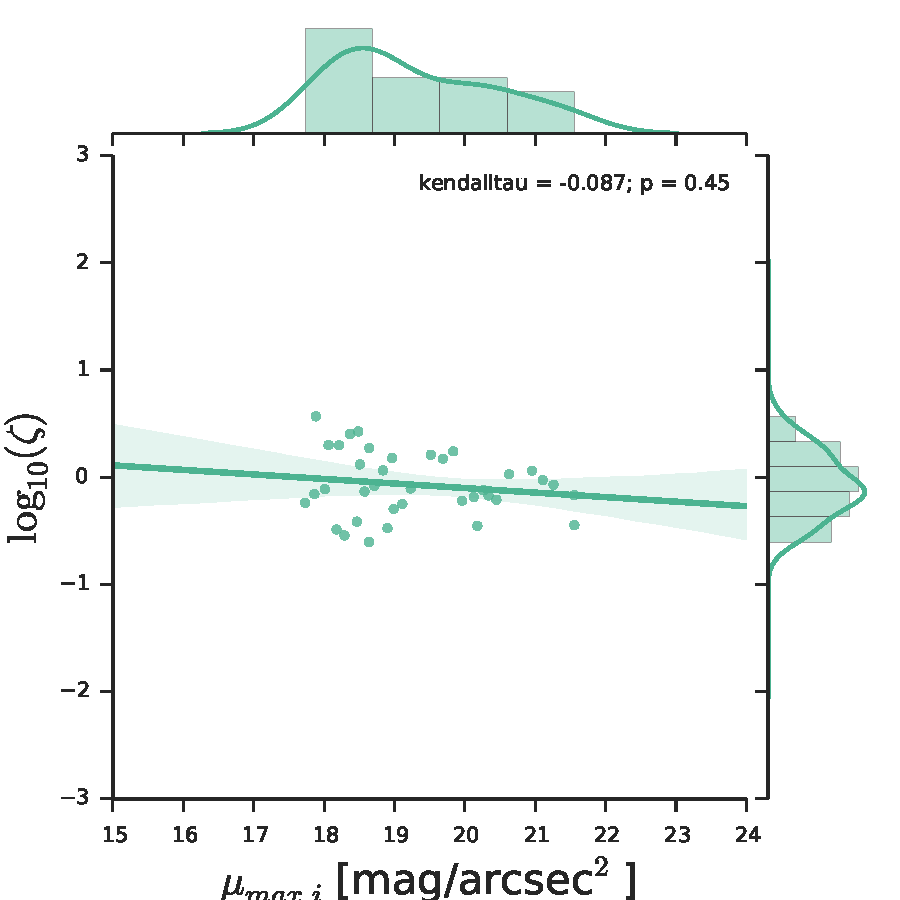
\includegraphics[width=0.50\textwidth]{figures/zeta_mu.pdf}
\caption{All fits for the vote fraction dropoff parameter $\zeta$ for $f_\textrm{features}$ in the \ferengi{} galaxies as a function of surface brightness. This includes only the 37~galaxies with a reasonably bounded range on the dropoff ($-10<\log(\zeta)<10$) and sufficient points to fit the function.}
\label{fig:zeta_mu}
\end{figure}

We fit the data in Figure~\ref{fig:zeta_mu} with a linear function such that:

\begin{equation}
\log_{10}(\hat\zeta) = \zeta_0 + (\zeta_1 \times \mu),
\label{eqn:zetafit}
\end{equation}

\noindent where $\hat\zeta$ is the correction factor applied to each galaxy as a function of surface brightness. The best-fit parameters to the linear fit (from least-squares optimization) are $\zeta_0=0.1$, $\zeta_1=1.4$. To make the final debiased correction, we modify the simple exponential form of Equation~\ref{eqn:fzeta} to bound the debiased vote fractions between $f$ and 1:

\begin{equation}
f_\textrm{features,debiased} = 1 - (1 - f)e^{\frac{z-z_0}{\hat\zeta}}.
\label{eqn:fzeta_mod}
\end{equation}

\subsection{Results of $\zeta$ approach}\label{ssec:zeta_results}

\begin{figure}
\begin{center}
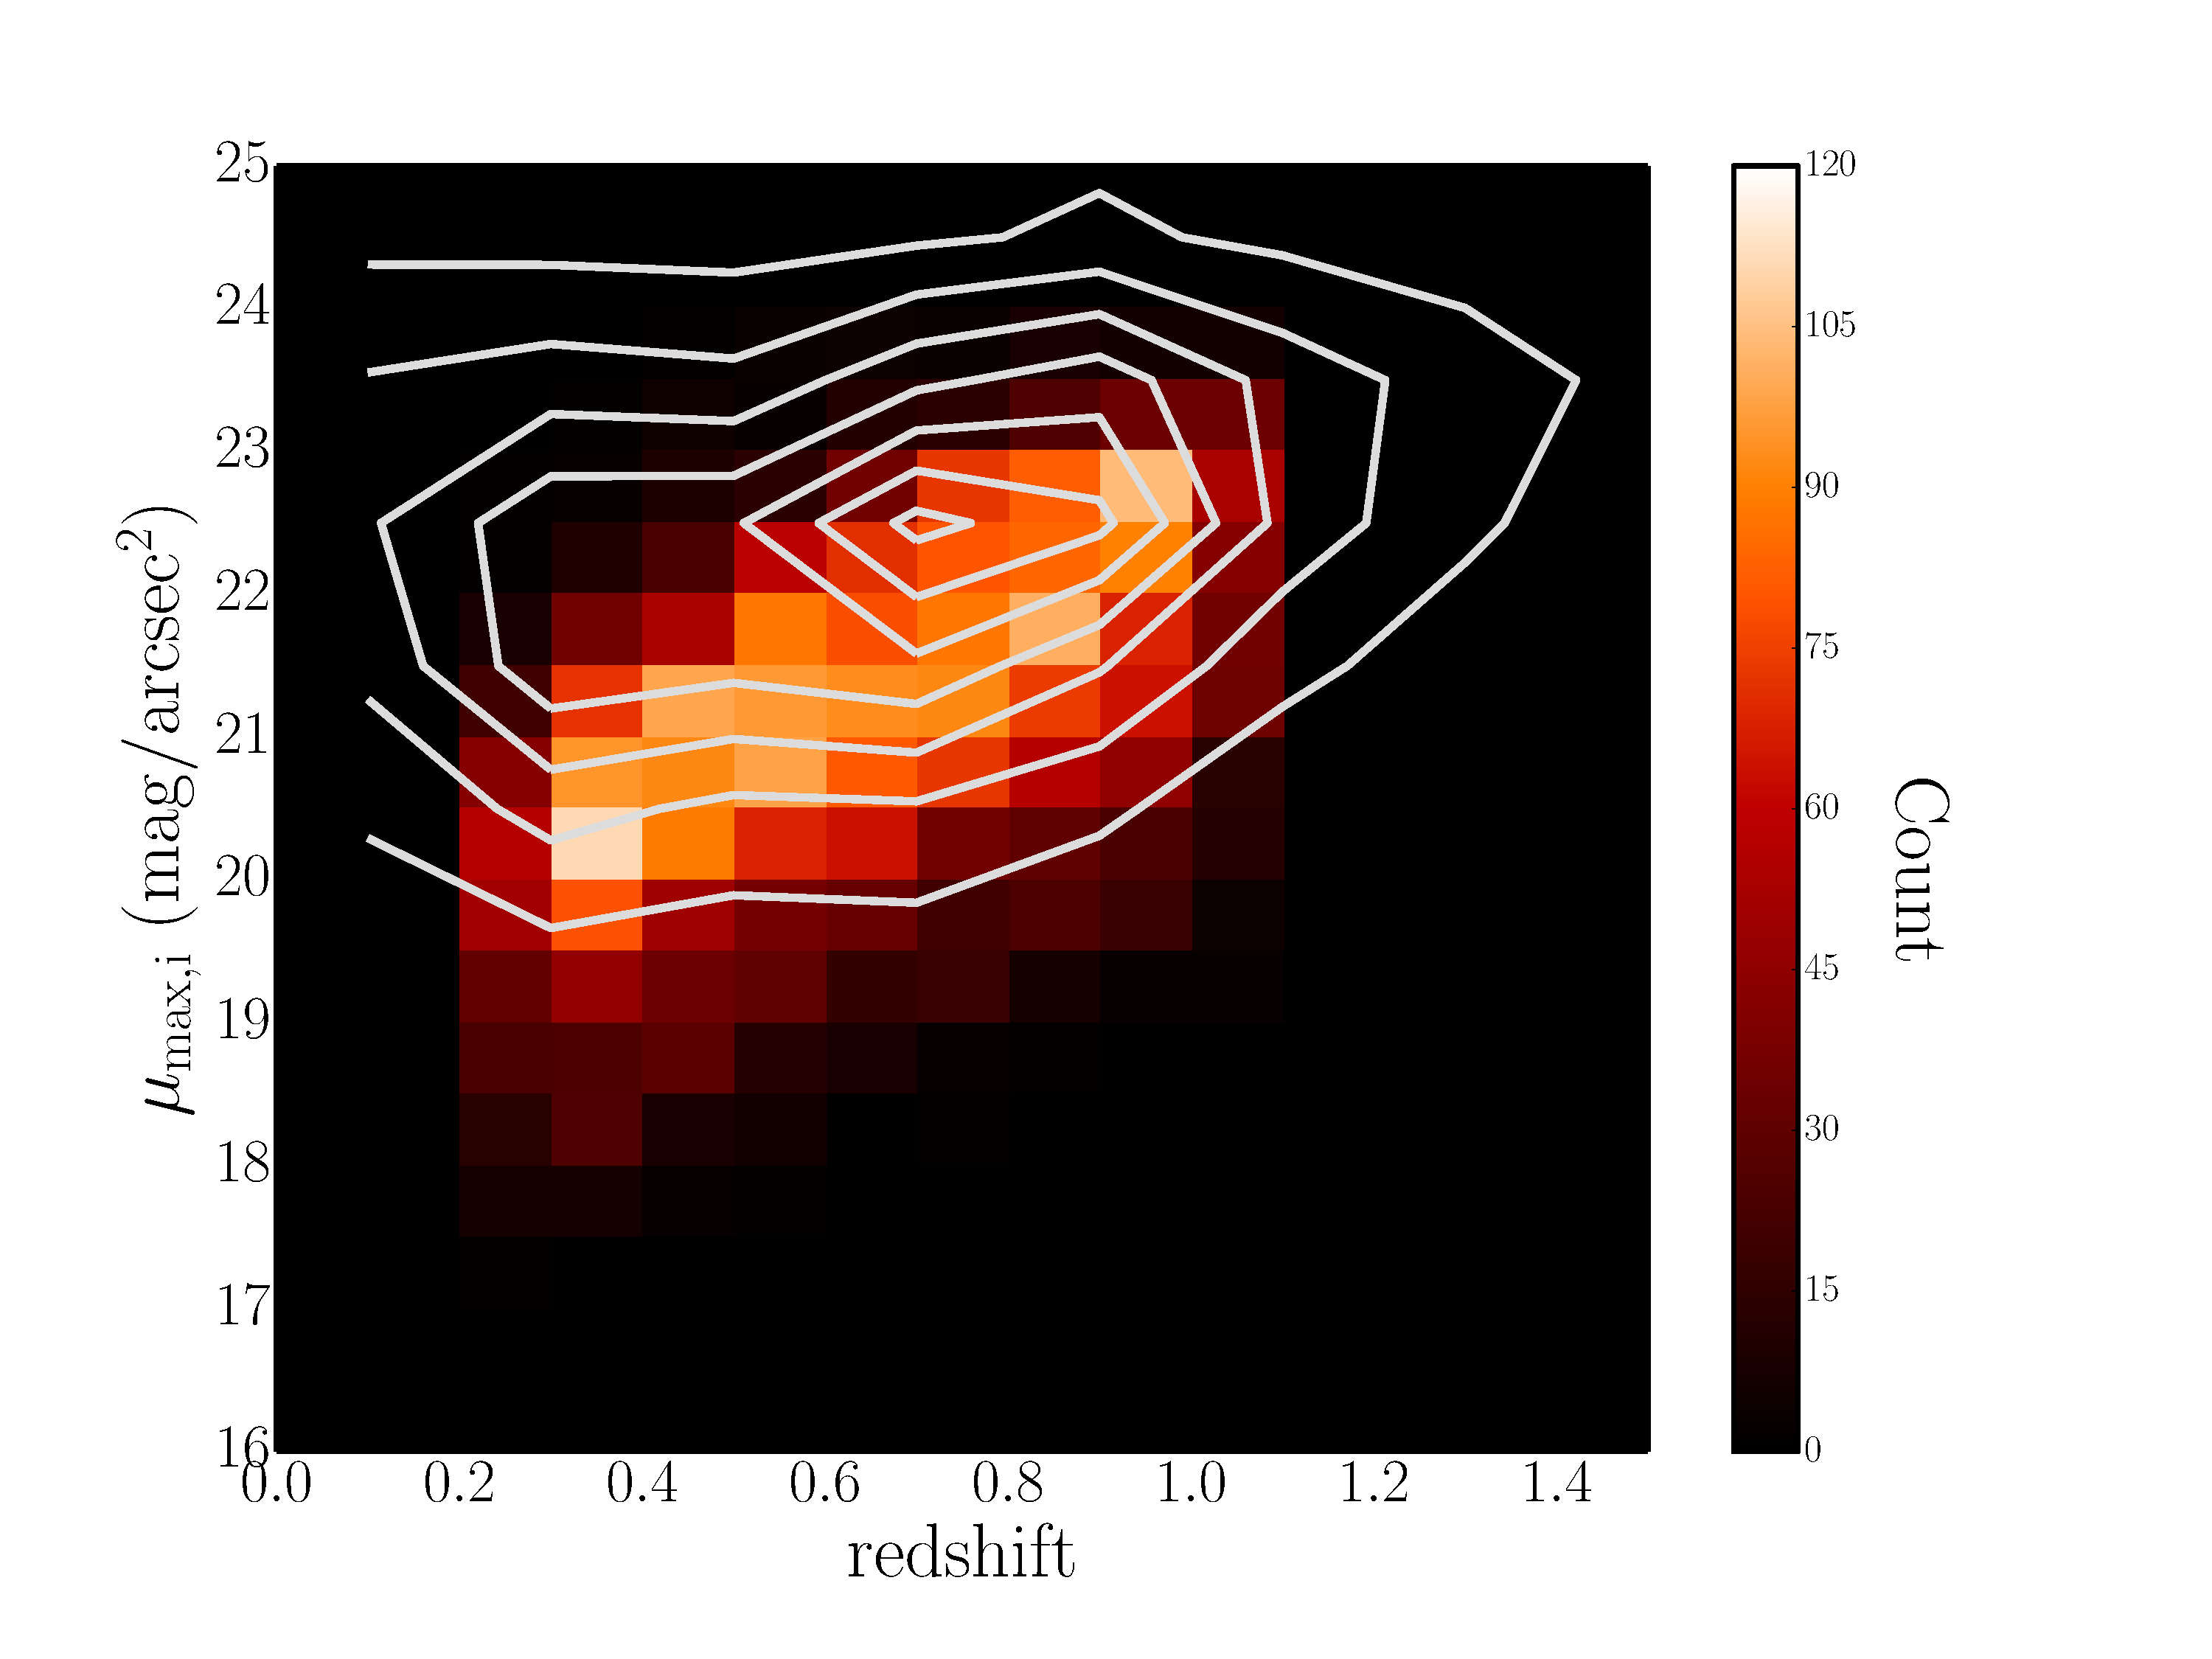
\includegraphics[width=0.5\textwidth]{figures/eye_of_sauron.pdf}
\caption{Surface brightness vs. redshift of 118,083 galaxies in the ACS sample. The white grid denotes the surface brightness and redshift range of the \ferengi{} images, subdivided in bins corresponding to fixed ranges used for analysis in Figure~\ref{fig:p_vs_p}.}
\label{fig:sb_redshift}
\end{center}
\end{figure}

\begin{figure*}
\centering
\subfigure{[a]\label{fig:6a}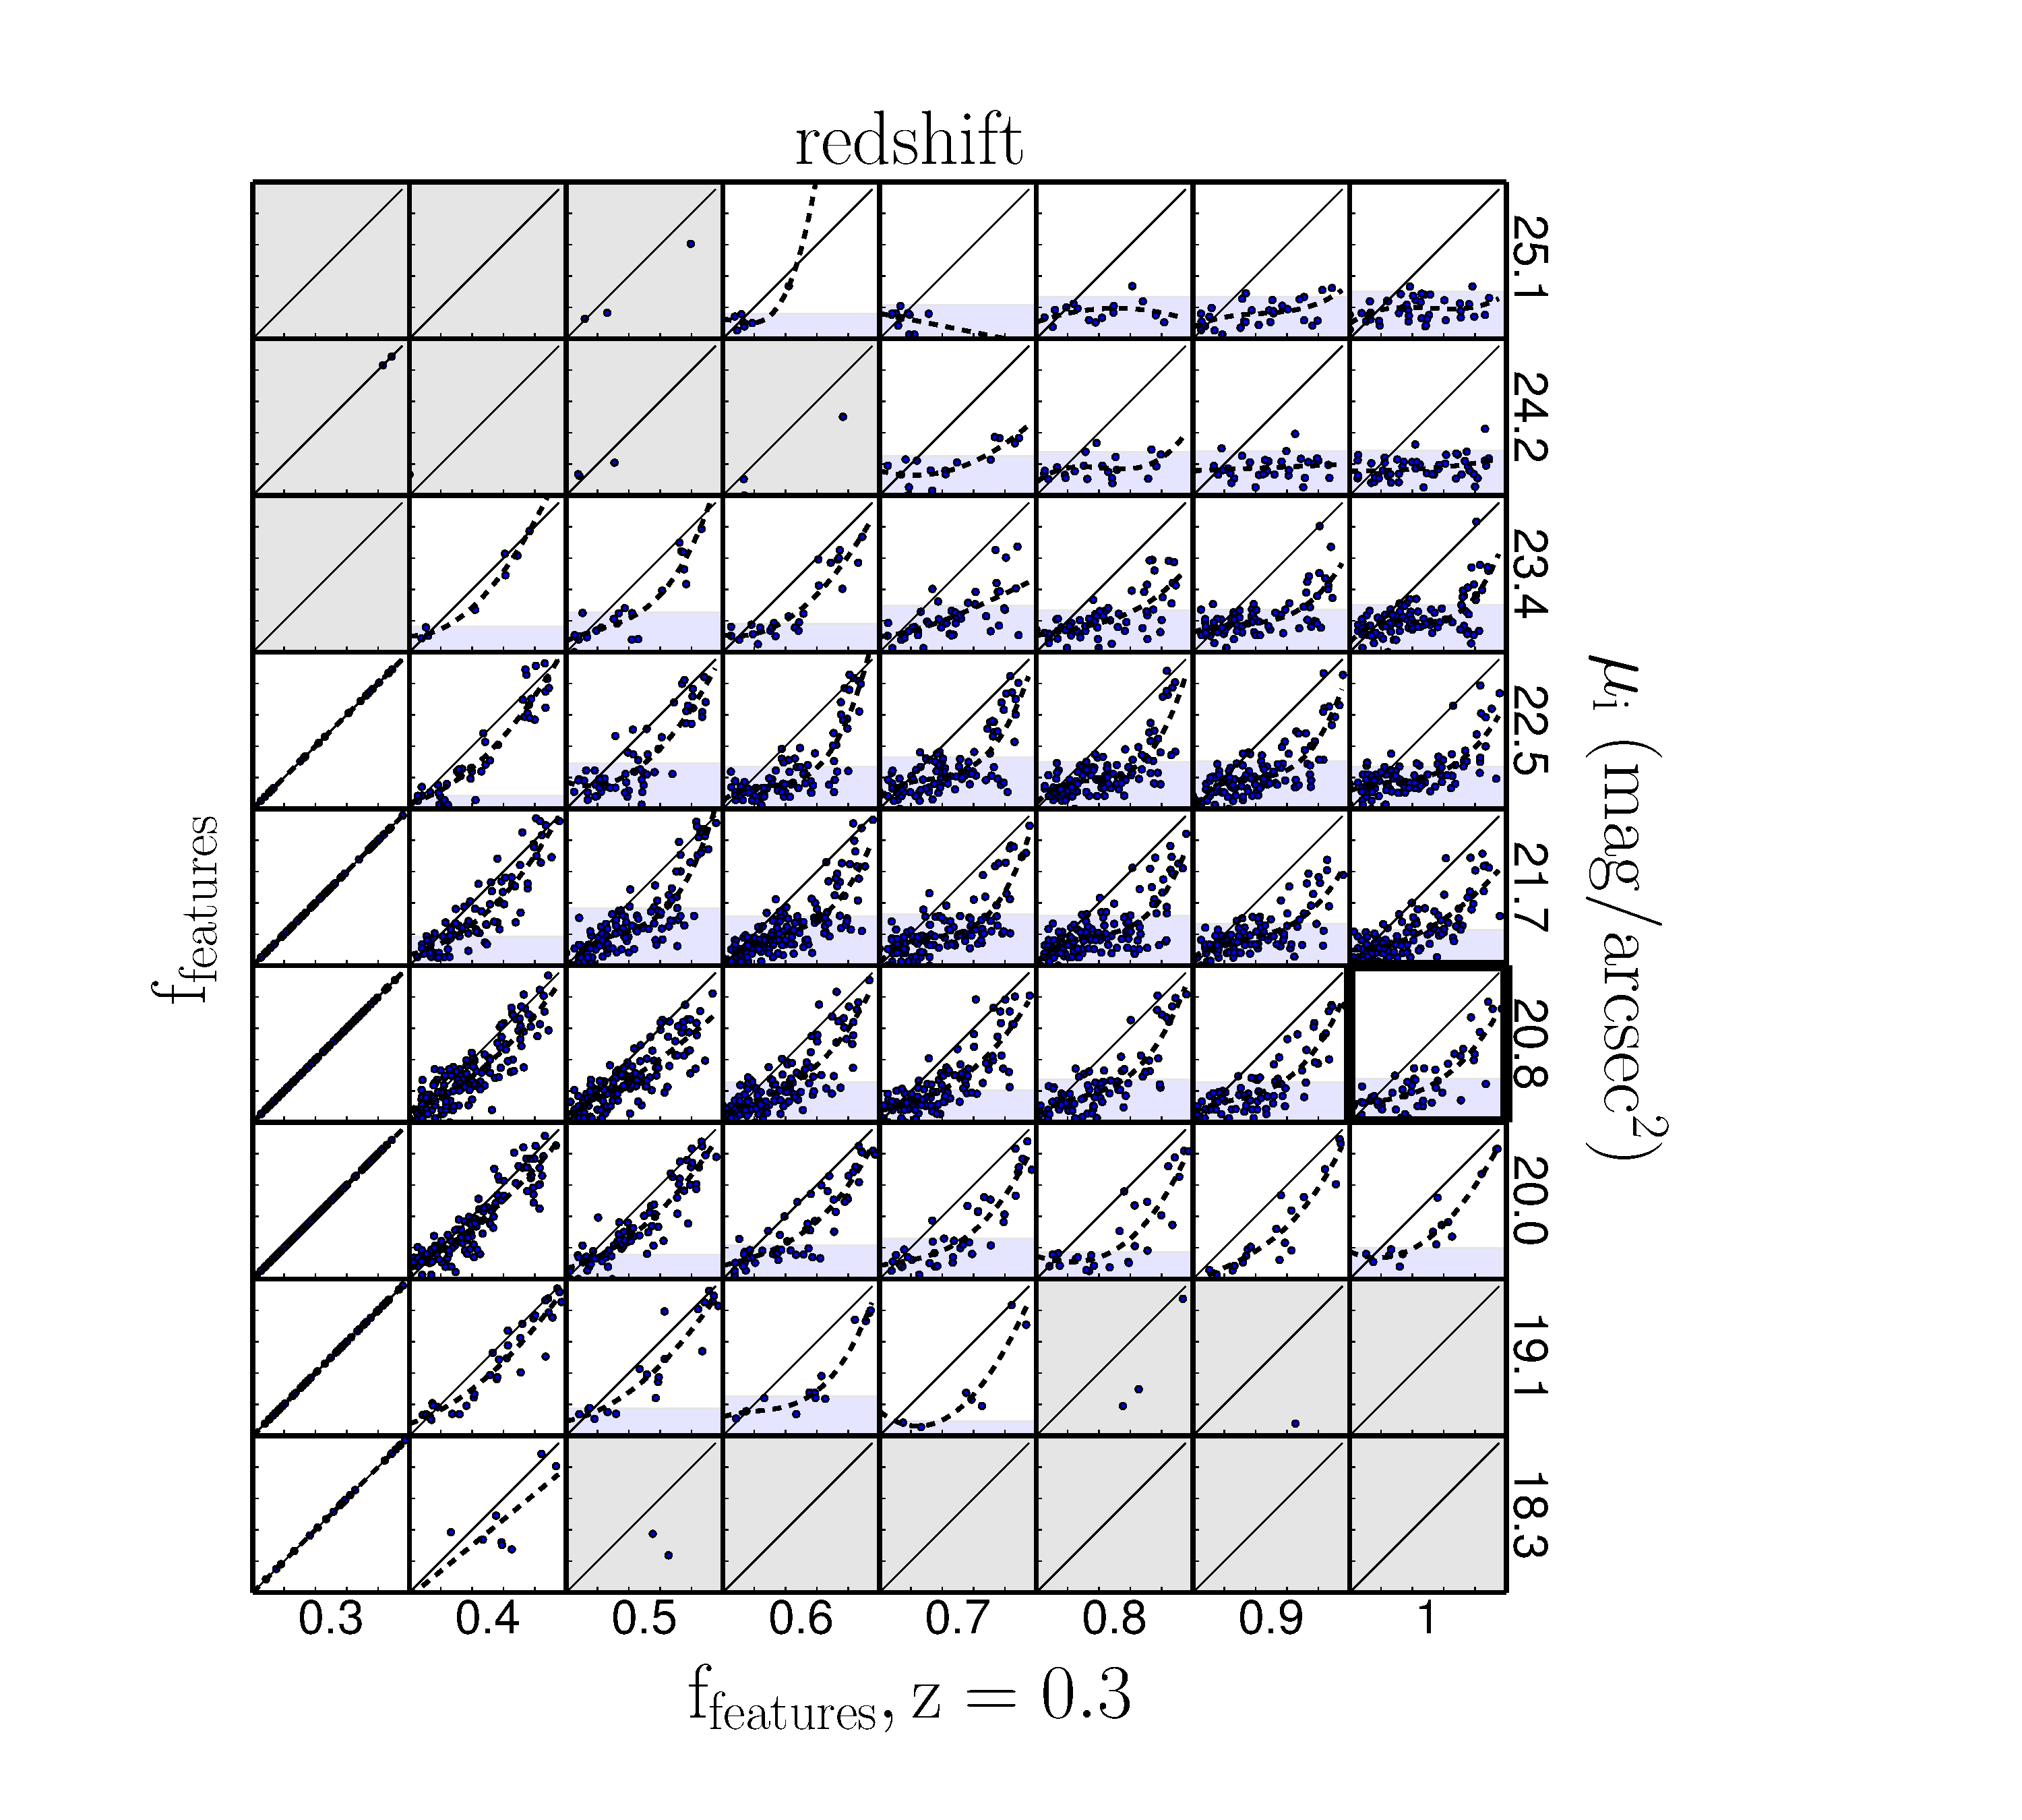
\includegraphics[width=0.5\textwidth]{figures/p_vs_p_SB_redshift.pdf}}
\subfigure{[b]\label{fig:6b}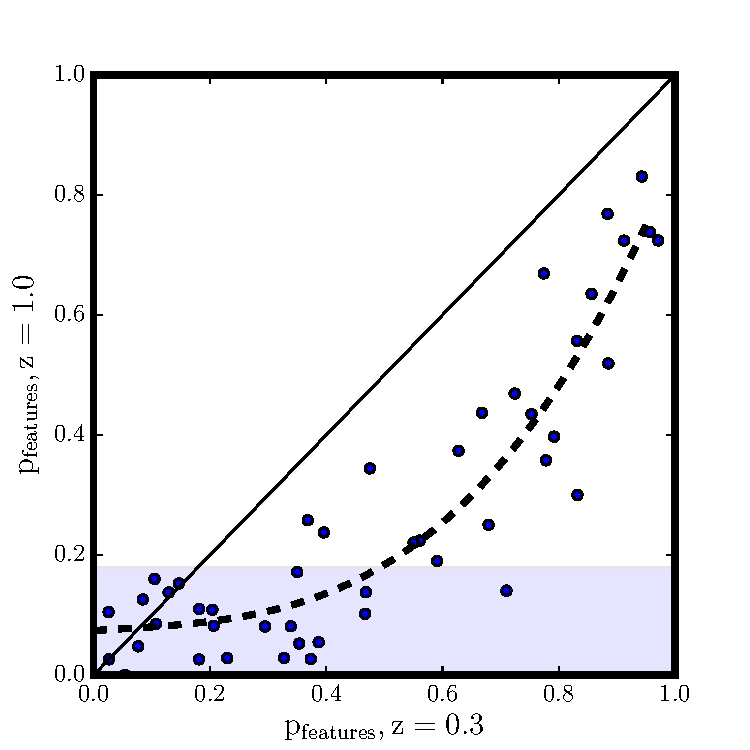
\includegraphics[width=0.4\textwidth]{figures/z1_mu20_subplot1.pdf}}
\\
\subfigure{[c]\label{fig:6c}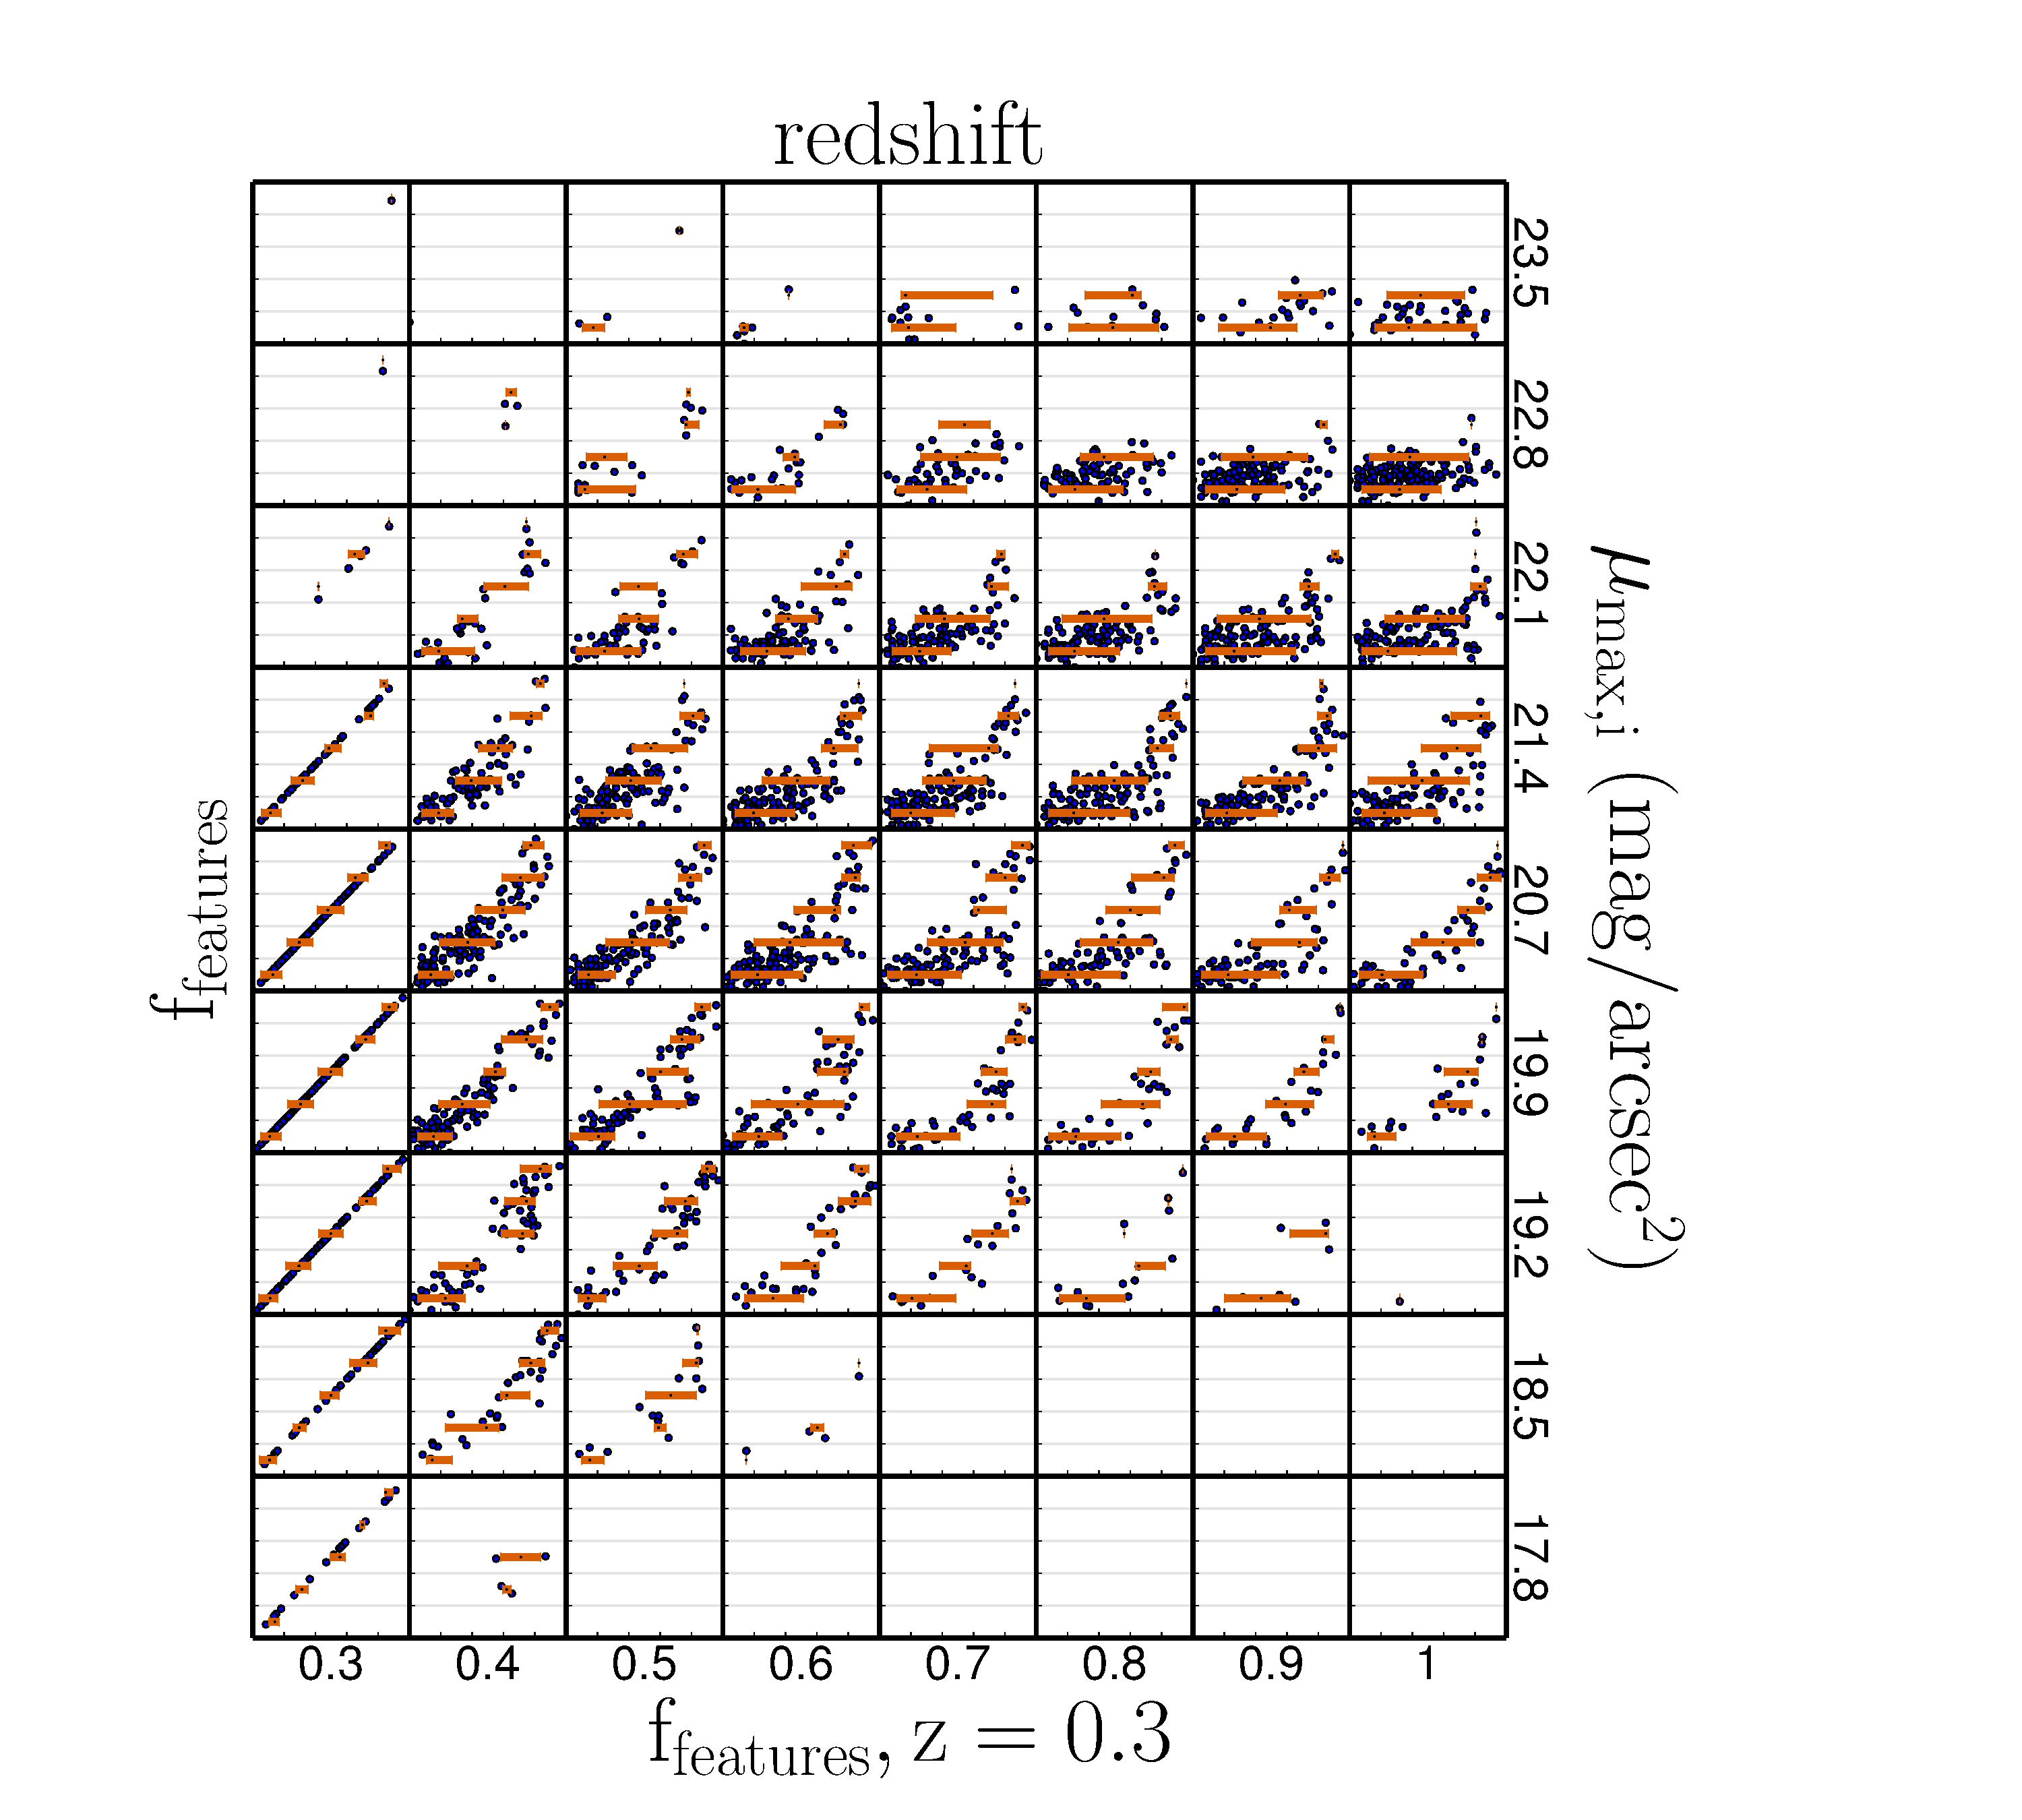
\includegraphics[width=0.5\textwidth]{figures/orangebars.pdf}}
\subfigure{[d]\label{fig:6d}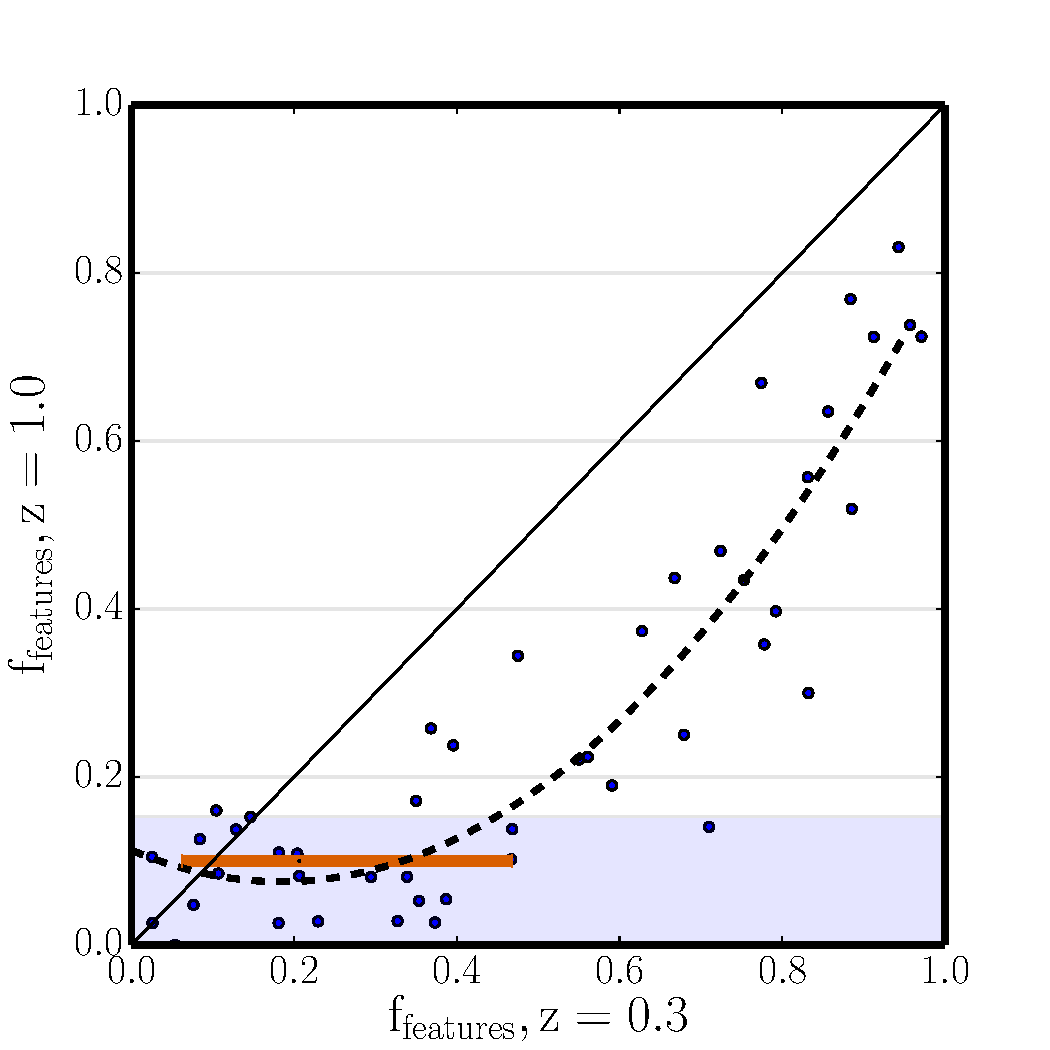
\includegraphics[width=0.4\textwidth]{figures/z1_mu20_subplot2.pdf}}
\caption{Effects of redshift bias in 3,950 images in the \ferengi{} sample. [a]: Each point in a given redshift and surface brightness bin represents a unique galaxy. On the $y$-axis in each bin is the \pfeatures{} value of the image of that galaxy redshifted to the value corresponding to that redshift bin. On the $x$-axis is the \pfeatures{} value of the image of the same galaxy redshifted to $z=0.3$. The dashed black lines represent the best-fit polynomials to the data in each square. The solid black line represents \pfeaturesz=\pfeaturesrest. Regions in which there is a single-valued relationship between \pfeatures{} at high redshift and at $z=0.3$ are white; those in which there is not are blue, and those with not enough data ($N<5$) are gray. [b]: A larger version of the dark-outlined square in [a], containing \ferengi{} galaxies that have been artificially redshifted to $z=1.0$ and have surface brightnesses between $20.3 < \mu < 21.0$ $\rm (mag/arcsec^2)$. [c]: The same data as [a] is shown. Each $z,\mu$ bin is divided into 4 sub-bins to determine the range of intrinsic \pfeaturesrest{} for a given range of observed \pfeaturesz{} values. In each sub-bin, the orange bars represent the inner 80$^\mathrm{th}$ percentiles of the data, the boundaries of which are the lower and upper limits of the debiased values. [d]: The same data as [b], but highlighting the upper and lower limit regions.}
\label{fig:p_vs_p}
\end{figure*}

In Figure~\ref{fig:p_vs_p} we examine the change in \pfeatures{} for the \ferengi{} galaxies relative to their lowest simulated redshift. In this analysis, only galaxies whose lowest simulated redshift image was $z_\mathrm{sim}=0.3$ were used (see Table \ref{tbl:ferengivalues}), and only those which had detectable surface brightness measurements in \sextractor; this includes 3,950 of the total 6,466 images. For each simulated redshift value $z$, and at a fixed surface brightness $\mu$, we plot \pfeaturesz, the value measured at that simulated redshift, vs \pfeaturesrest, the value measured for the same galaxy imaged at $z=0.3$. 
 
Our objective is to use these data to predict, for a galaxy with a measured \pfeaturesz{} value, what its \pfeatures{} value \emph{would have been} if it had been viewed at $z=0.3$. This predicted value is defined as the debiased vote fraction \pfeaturesdebiased, and is calculated by applying a correction to the measured value of \pfeatures, determined by the $\zeta$ function described in the previous section. A reliable predicted value can be obtained so long as the relationship between \pfeaturesz{} and \pfeaturesrest{} is single-valued; that is, for a given \pfeaturesz, there is exactly one corresponding value of \pfeatures{} at $z=0.3$. 

Figure~\ref{fig:p_vs_p} shows that the relationship between \pfeaturesz{} and \pfeaturesrest{} is \emph{not} always single valued; hence, it is not appropriate to correct galaxies that lie in certain regions of surface brightness/redshift/\pfeatures{} space. These regions tend to have low \pfeatures{} values at high redshift, but a wide range of values at $z=0.3$. These regions contain two morphological types of galaxies: First are genuine ellipticals, which have low values of \pfeatures{} at both high and low redshift. Second are disks whose features become washed out at high redshift; hence their \pfeatures{} value at $z=0.3$ may be quite high, while the value observed at high redshift is very low. This effect is strongest at high $z$ and low $\mu$, where features become nearly impossible to discern in the images.

Our criteria for determining whether a region of this space is single-valued, and therefore correctable, is as follows: In each surface brightness and redshift bin, we model the relationship between \pfeaturesz{} and \pfeaturesrest{} by fitting the data with a polynomial of degrees 3, 2, and 1, and use the best fit out of the three. These fits are shown as the dashed black lines in Figure~\ref{fig:6a}. Any flat regions of the polynomial fits are areas in which there is not a clear single-valued relationship between \pfeaturesz{} and \pfeaturesrest; we quantify this by setting a minimum slope cut of 0.4. Any data in which the polynomial fit has a slope less than this value is considered \emph{not} one-to-one, and therefore \pfeaturesz{} cannot be boosted to its \pfeaturesrest{} value. We refer to galaxies in this region as the \emph{lower limit} sample. These regions are highlighted in blue in Figure~\ref{fig:6a}. Uncolored (white) regions of the plot have sufficiently high slopes for us to consider the relationship to be single-valued; galaxies in these regions are considered ``correctable'', and only these are used in measuring the parameters for the $\zeta$ function (Section~\ref{ssec:zeta}). Only surface brightness/redshift bins with at least 5 galaxies were considered; regions with fewer than 5 galaxies we consider to have ``not enough information'' to determine the \pfeaturesz{} and \pfeaturesrest{} relationship, colored gray in Figure~\ref{fig:6a}.

The unshaded regions in Figure~\ref{fig:6a} define discrete ranges of redshift, surface brightness, and \pfeatures{} a galaxy must have in order for the $\zeta$ approach to be confidentely applied to a galaxy in the GZH sample. While the appropriate correctable regions were defined discretely, we assume the true correctable region is a smooth function of $z$, $\mu$, and \pfeatures{}. To define this smooth space, we generate a convex hull that encloses the correctable and lower-limit \ferengi{} galaxies in $z$-$\mu$-\pfeatures{} space. The boundaries are then adjusted until the contamination from both groups is minimized. We use the resulting hulls to define the correctable and lower-limit regions for categorizing the \hst{} galaxies. The results of this method and final categorization of the \hst{} sample is displayed in Table~\ref{tbl:hubble_debiasable}. Of the galaxies at redshift higher than $z=z_{0}=0.3$, 17\% of these are able to be debiased using the $\zeta$ method, 27\% cannot be debiased, and 56\% cannot be determined, due to a lack of redshift or information or due to a lack of \ferengi{} data corresponding to those galaxies' redshift/surface brightness values.

For the ``lower-limit'' galaxies for which we cannot confidently assign a single debiased \pfeatures{} value, we instead determine a likely \emph{range} of debiased values, using a method visualized in Figure~\ref{fig:6c}. Here we again use the \ferengi{} simulated data to analyze the range of intrinsic \pfeaturesrest{} values for any given observed \pfeatures{} value, again as a function of surface brightness and redshift. In each $z$,$\mu$ bin, we examine the spread of intrinsic values of \pfeaturesrest{} for 4 ranges of observed \pfeatures. We quantify the range of intrinsic values as the inner 80\% of the data; this range is represented by the orange bars in Figure~\ref{fig:6c}. For any galaxy which can't be directly debiased by the $\zeta$ method, then, we use these ranges to denote the upper and lower limits on what we expect \pfeaturesrest{} to be for any observed value of \pfeatures. 

\begin{table}
\center
\caption{Distribution of \ferengi{} images analysed in Figure~\ref{fig:p_vs_p}. Correctable images have a single-valued relationship between their measured \pfeatures{} values at high and low redshifts (white regions in Figure~\ref{fig:p_vs_p}). Images with only a lower-limit on \pfeatures{} have a non single-valued relationship (blue regions). NEI images have undetermined relationships due to a lack of data ($N<5$) in their corresponding $z$-$\mu$ bins (gray regions).\label{tbl:ferengi_corrections}}
\begin{tabular}{lrr}
\hline \hline
				                   & N       & \% \\
\hline 
Correctable                        & 1,884   & 48\% \\
Lower-limit                        & 1,986   & 50\% \\
NEI                                & 80      &  2\%\\
Total                              & 3,950   & 100\% \\
\hline \hline
\end{tabular}
\end{table}

\subsection{Challenges of debiasing questions beyond ``smooth or features''}

As with the HST images, each FERENGI subject has a varying number of users answering the various questions in the hierarchical decision tree. Every user answers the first question, ``Is the galaxy smooth and rounded, with no sign of a disk?''; as such the vote fractions $\rm p_{smooth}, p_{features}$, and $\rm p_{artifact}$ are all computed with the minimum statistical error for any question, with roughly 40 total answers (see Section~\ref{sec:interface}). The number of users to answer any subsequent question, however, is always equal to or less than the number to answer the preceding question. The average number of responses per task for fourth- or fifth-tier questions such as spiral arm structure (Tasks 12--14) is only $4\pm4$ for the FERENGI sample; while this is distribution is strongly bimodal (reflecting the true morphologies of selected galaxies), the very low absolute numbers of votes introduce very high variance when attempting to calculate a statistical correction.

In the FERENGI data, these numbers severely limit the amount of information we can extract for the higher-tier questions. The debiasing technique used (Section~\ref{ssec:zeta}) require that at least 10~users answer each question for a galaxy image at $z=0.3$ \emph{and} its image at higher redshift. This requirement is by default met by all galaxies when analyzing the first question, since it is asked of all users. This requirement is often \emph{not} met for questions beyond Task~01; on average 59\% of the galaxies do not have sufficient data to measure a correction, as compared to 2\% acheived for Task~01 (see Table~\ref{tbl:ferengi_corrections}). Of the remaining FERENGI galaxies which did meet this requirement, the data available in each redshift-surface brightness bin were not tightly correlated between $p_{task,z=0.3}$ and $p_{task,z}$, and relationships between the two could not be fit with high confidence. We use these galaxies to compute $\zeta$ for each Task, and find the p-values for the resulting functions between $placeholder < p < placeholder$, which we consider insufficient for deriving a correction. We show an example of this in Section \ref{sec:ferengi_bar}, where we show results of measuring $\zeta$ for $p_{\rm bar}$ in Task~03. For this reason we only offer debiased vote fractions for Task~01 (smooth/features/artifact). 

\begin{table*}
\caption{Correctable fractions for the top-level task in GZH, split by survey.}\label{tbl:hubble_debiasable}
\begin{tabular}{lcrrrrrrr}
\hline\hline
                                   & Correction type & AEGIS   & COSMOS & GEMS & GOODS-N & GOODS-S    & SDSS    & Total \\
\hline
Correctable                        & 0               & 1,654   & 15,170 & 1,837 & 993    & 835     	& 0       & 20,489\\
Lower-limit                        & 1               & 1,917   & 26,113 & 2,423 & 1,385  & 1,282   	& 0       & 33,120\\
No Correction Needed ($z \le 0.3$) & 2               & 955     & 11,926 & 1,175 & 415    & 400     	& 37,545  & 52,416\\ 
NEI                                & 3               & 2,847   & 34,511 & 3,308 & 2,535  & 2,523   	& 0       & 45,724\\
No Redshift Information            & 4               & 1,134   & 5,088  & 561   & 687    & 102   		& 14,316  & 21,888\\
Total                              &                 & 8,507   & 92,808 & 9,304 & 6,015  & 5,142   	& 51,861  & 173,637\\
\hline\hline
\end{tabular}
\end{table*}

\begin{figure*}
\center
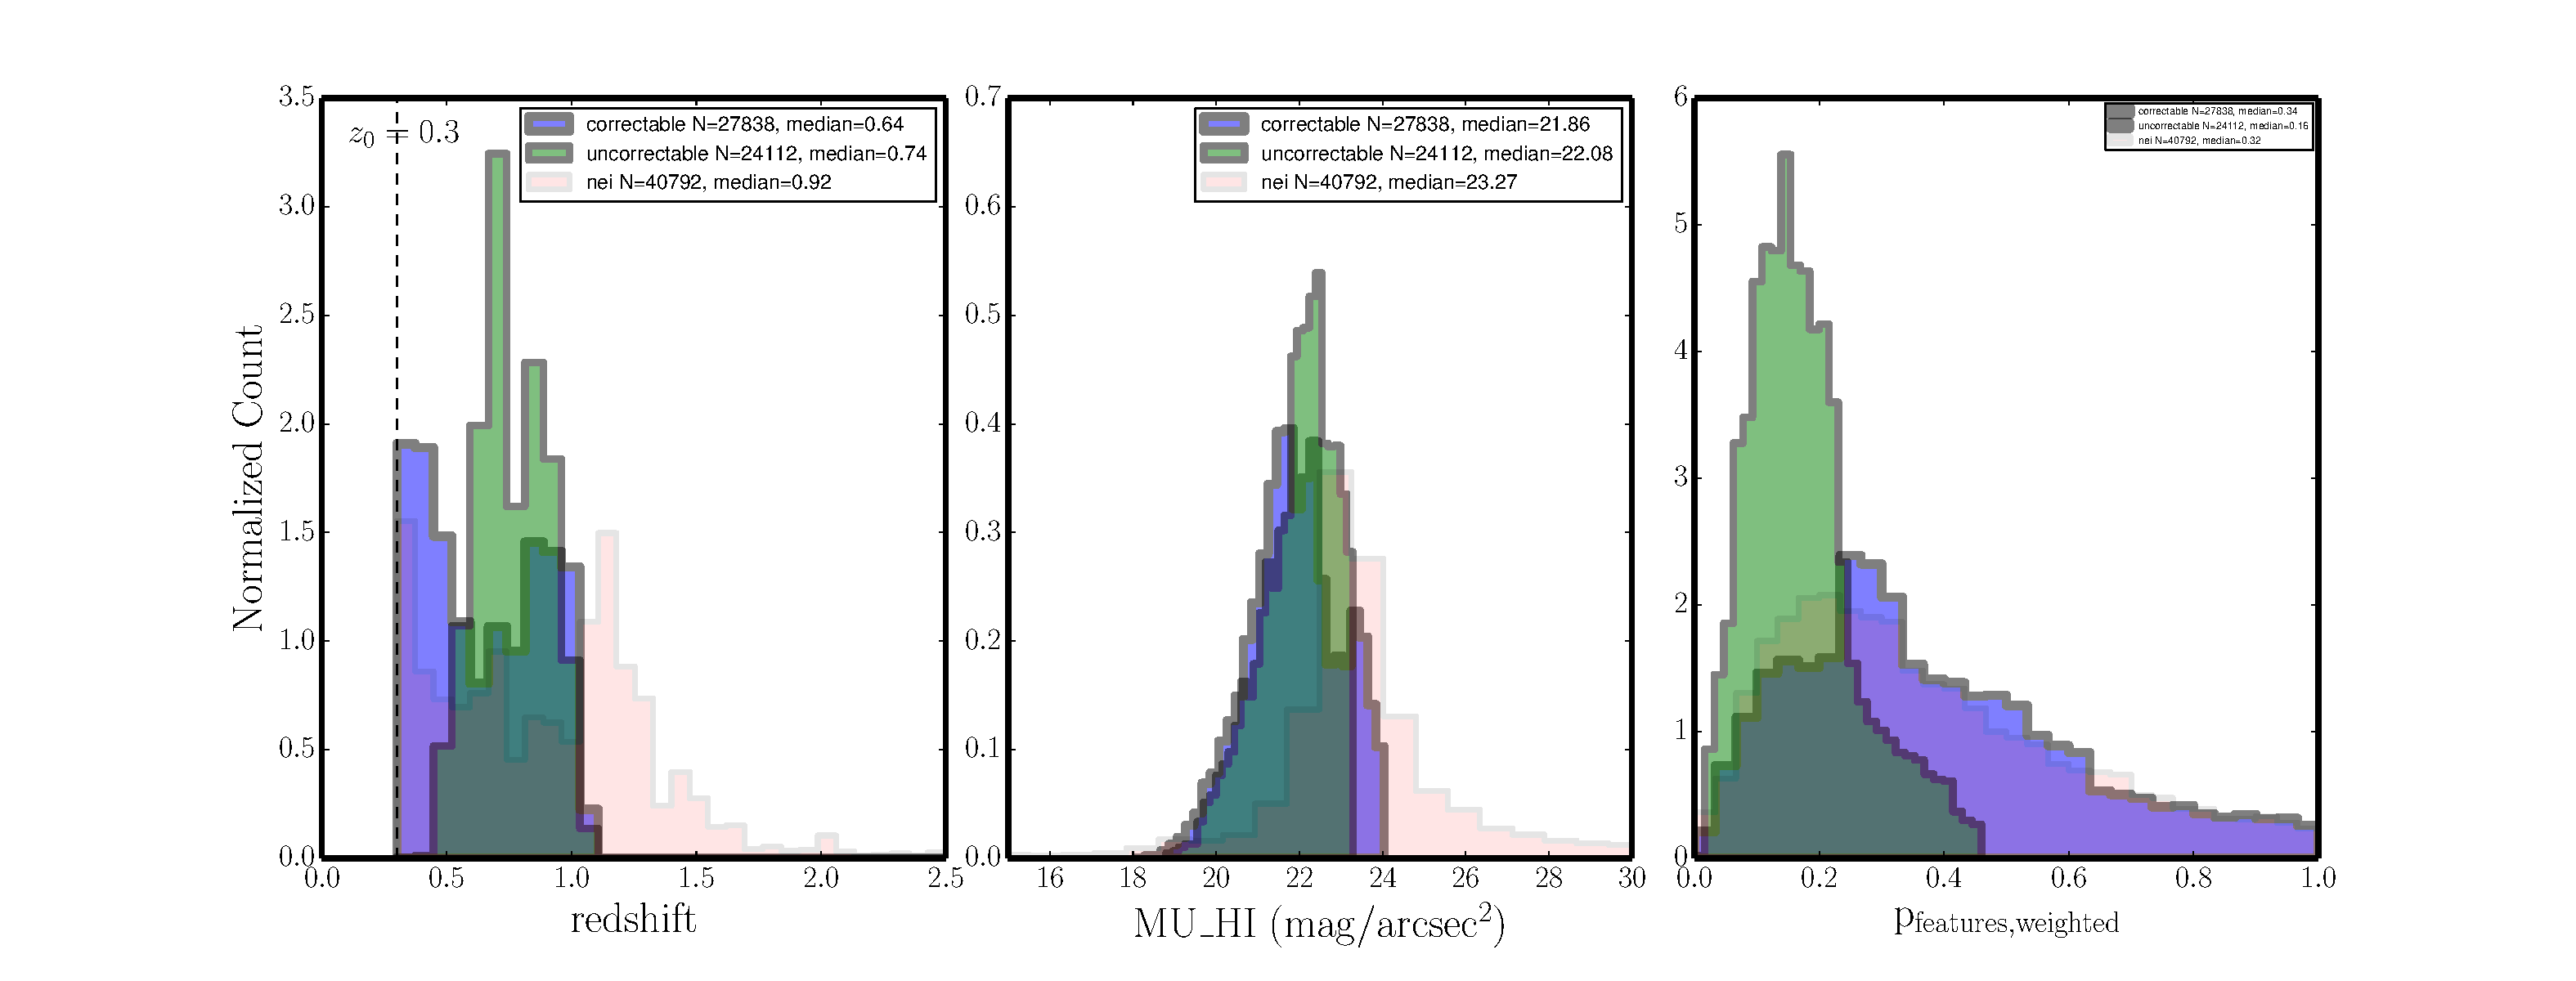
\includegraphics[width=\textwidth]{figures/hubble_z_mu_p_distributions.pdf}
\caption{Distributions of redshift, surface brightness, and $p_{features}$ for correctable (purple), lower-limit (green), and NEI (pink) galaxies in the full GZH sample. The lower-limit galaxies have higher redshifts, slightly lower surface brightness, and lower values of $p_{features}$ on average than the correctable galaxies. The long tail of NEI galaxies in redshift and surface brightness demonstrates the limits of the \ferengi{} sample, for which there is no data at $z>1$ or $\mu>24$.}
\label{fig:z_mu_p}
\end{figure*}

\begin{figure*}
\center
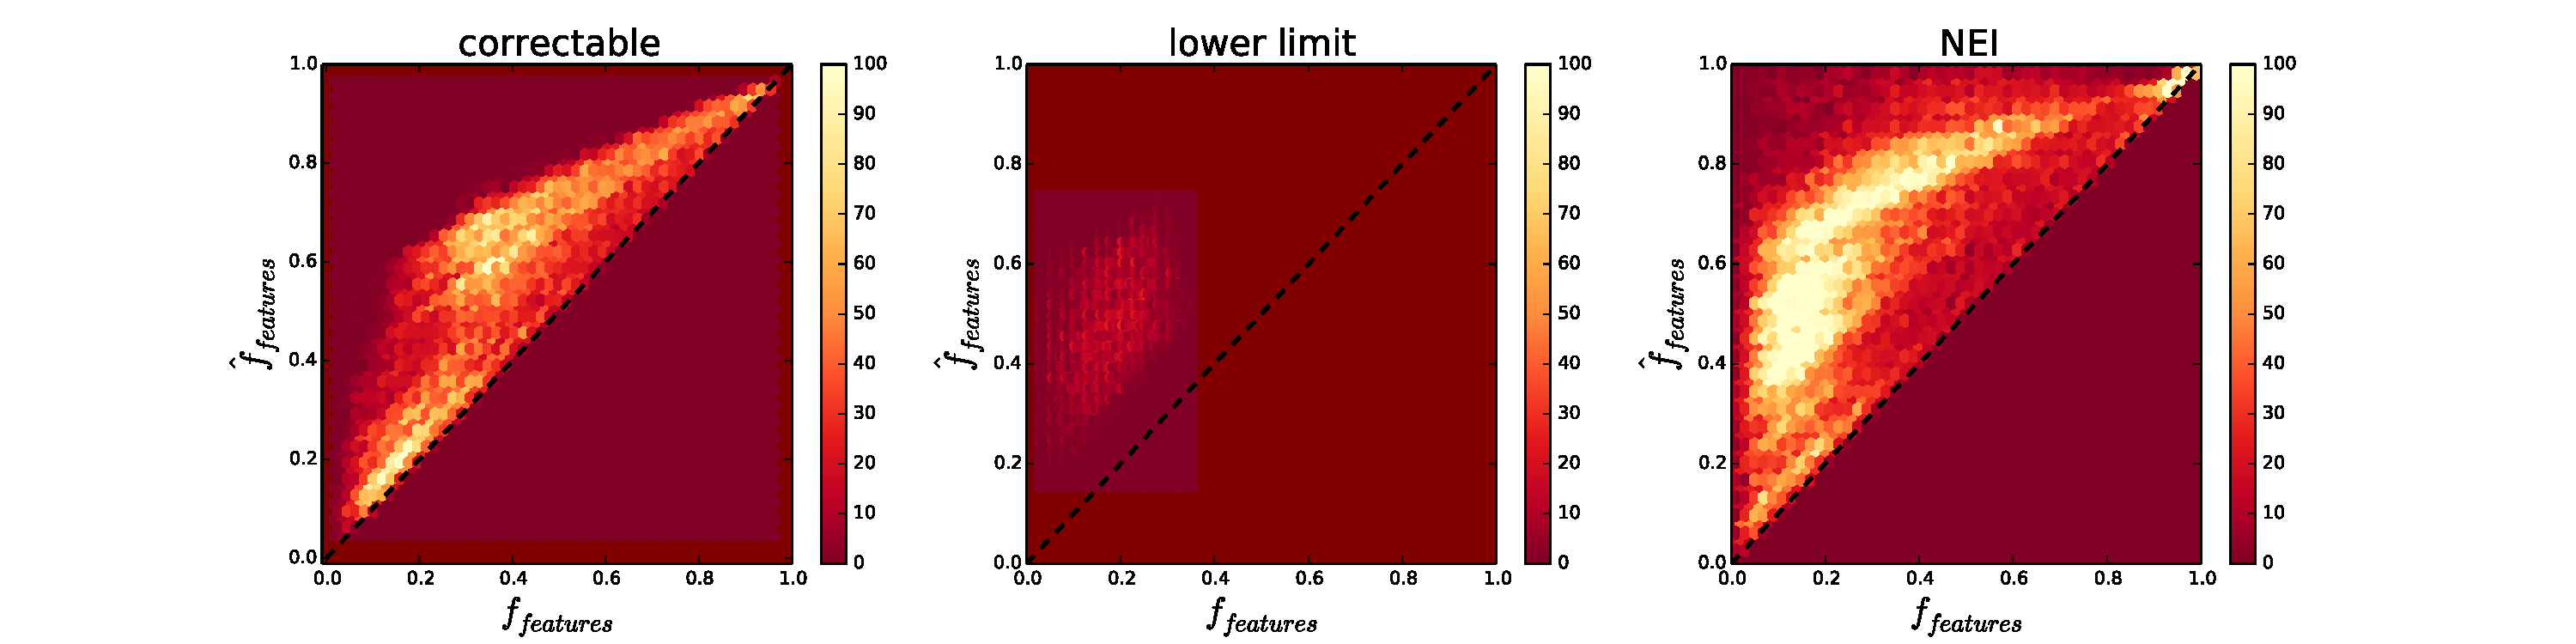
\includegraphics[width=\textwidth]{figures/debiased_corrections.pdf}
\caption{Debiased $p_{features}$ corrected to $z=0.3$ vs weighted $p_{features}$ for the correctable (left), lower-limit (middle), and NEI (right) galaxies in the GZH sample.}
\label{fig:debiased_corrections}
\end{figure*}


%\subsection{Results of FERENGI analysis}
%
%{\bf Old text from Taiwan workshop}
%
%We show here the preliminary results of GZH classifications of images of galaxies placed at artificial redshifts. Figure~\ref{fig:ferengi_results_fake} shows the range of change of vote fractions for the change of \pfeatures{} with redshift, for galaxies with different vote fraction levels, three ranges of surface-brightness levels and 7~evolutionary corrections (this last bit is indicated by the colour). 
%
%%-----------------------------------------------------------------------------------------------------------------------------------
%\begin{figure}
%\begin{center}
%
%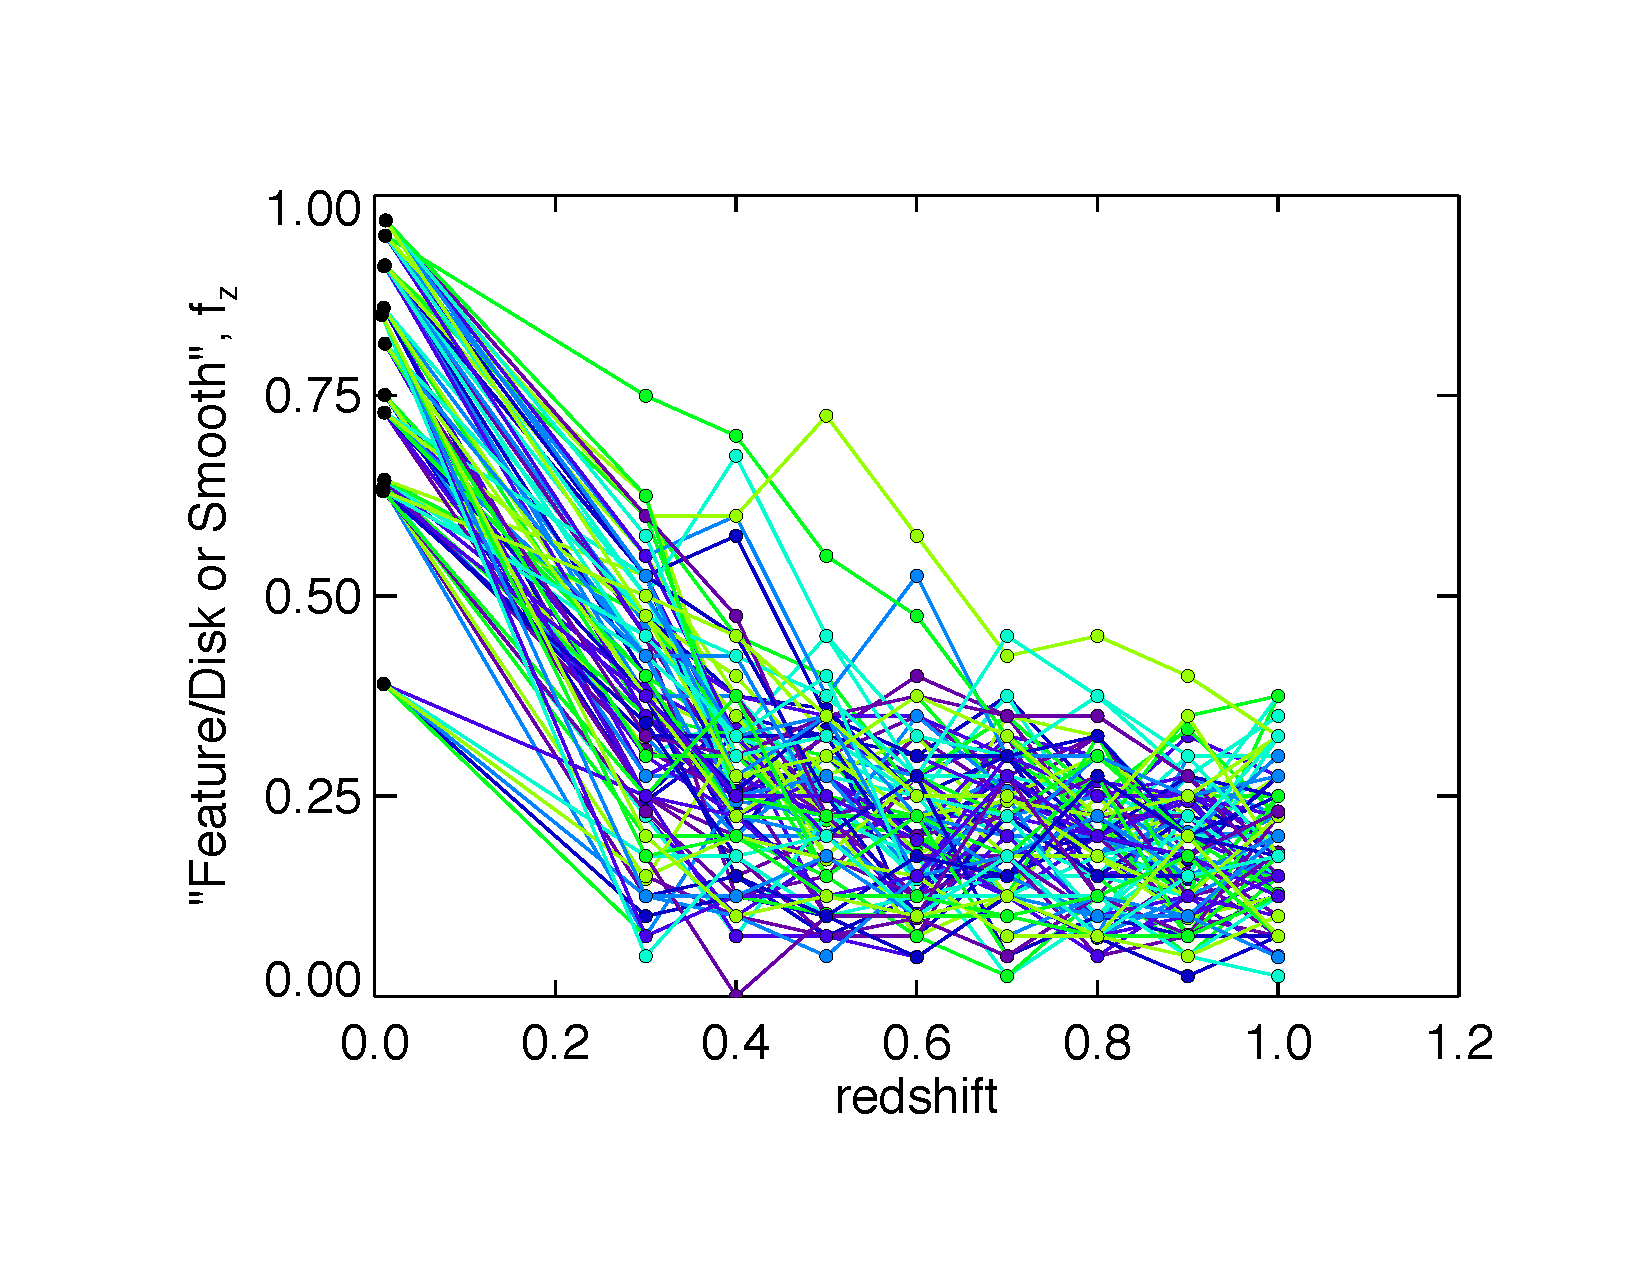
\includegraphics[width=0.45\textwidth]{figures/somewhat_fake_results.pdf}
%
%\caption{Preliminary results of the \ferengi{} redshifting exercise. WARNING NO USER WEIGHTING.... For a range of vote fraction levels with three surface-brightness levels and 7 evolutionary corrections each (the colours indicate evolutionary correction value with green being $e=0$, we show the range of evolution of the vote fractions for featured vs. smooth with redshift.}
%
%\label{fig:ferengi_results_fake}
%
%\end{center}
%\end{figure}
%%-----------------------------------------------------------------------------------------------------------------------------------

\section{The catalog}\label{sec:results}

The data release for GZH includes morphological data for 181,101~images (generated from a total of 150,771~unique galaxies). The full table can be accessed at \url{http://data.galaxyzoo.org}. We also include a secondary metadata table, which contains data from a variety of sources explained in Section \ref{sec:data}.

Each image is listed under a unique project ID (eg,~AHZ000001); the actual galaxy in the image is identified by the combination of the OBJNO and original survey. For each of the 55~responses in the GZH decision tree, the following classification data is provided: for each question, $\tt N_{votes}$ is the number of users to answer that question. For each unique answer, $\tt fraction$ is the fraction of users to select that answer ($\rm N_{answer}/N_{votes}$, and $\tt weighted$ is the weighted fraction, which takes into account user consistency (Section~\ref{ssec:weighting}). 

The GZH vote fractions can be largely dependent on the resolution of the image. Two otherwise morphologically identical galaxies which differ significantly in redshift, brightness, or size may result in very different vote fractions for any given question, given that many features of a galaxy are difficult to discern in less-resolved images (bars, spiral arms, disk structure, etc). For this reason, it is necessary to take caution utilizing vote fractions as cut-offs to determine morphological structure; we offer guidelines for careful classification in Section~\ref{sec:cookbook}. 

We corrected for the biases described for the first question of the GZH decision tree, which asks ``Is the galaxy smooth and round, with no sign of a disk?'' The method is described in Section~\ref{sec:debiasing}. For this question, we provide the additional parameters $\tt debiased$, $\tt lower~limit$, $\tt upper~limit$, and $\tt best$ vote fractions. The $\tt best$ fraction for $p_{features}$is chosen based on the categorization of the galaxy: if it is ``correctable'', $\tt best = debiased$, if a lower limit, $\tt best = lower~limit$, and if neither, $\tt best = weighted$. 

The debiased and best vote fractions for $\tt p_{smooth}$ were calculated on the critera that vote fractions for all answers must sum to unity. Explicitly: $\tt p_{smooth} = 1 - p_{features} - p_{artifact}$. In some rare cases, representing  $<1\%$ of the sample, this requirement resulted in negative vote fractions for $\rm p_{smooth}$; these were cases in which the $\rm p_{features}$ vote fraction was boosted to a high value relative to the $\rm p_{artifact}$ vote fraction. In these cases, we enforce the restriction that the vote fractions must sum to 1 by raising $\rm p_{smooth}$ to a vote fraction of 0.0 and decreasing $\rm p_{features}$ accordingly. This correction was typically very small, with a median decrease/increase of $\rm p_{features}/p_{smooth}$ of $\Delta p = 0.04$.

We split the data products for GZH by the type of image being classified. Table~\ref{tbl:catalog_hst} contains the classifications for the \hst{} images from the AEGIS, COSMOS, and GEMS surveys, as well as 5-epoch deep imaging from the GOODS-N and GOODS-S surveys. This contains 118,425~galaxies and is the primary output from the GZH project. The next two tables have data for a small subset of 3,927~COSMOS~images that were re-processed to study the effect of color balance on morphological classification. Table~\ref{tbl:catalog_faded} has images that are desaturated to minimize the color contrast; Table~\ref{tbl:catalog_recoloured} has images with the red and blue color channels inverted. Table~\ref{tbl:catalog_goods_shallow} contains data for 6,144~galaxies with 2-epoch images from GOODS. These have been mostly supplanted in the main table with deeper 5-epoch GOODS imaging; however, there are 1,683~galaxies in the shallower imaging that were not classified in the deeper mosaics. This data can also be compared to the counterparts in Table~\ref{tbl:catalog_hst} to study the effect of depth on morphological classification. Tables~\ref{tbl:stripe82_single} and \ref{tbl:stripe82_coadd} contain data for the SDSS Stripe~82 single-depth and co-added images, respectively, that were classified using the GZH interface and decision tree. Finally, Table~\ref{tbl:fake_agn} contains classifications for images with artificial point sources intended to simulate the effect of a bright AGN, as used in \citet{sim14}.  


\tabletypesize{\scriptsize}
\begin{deluxetable*}{lllcrllllll|c}
\centering
\tablecolumns{13}
\tablewidth{0pc}
\tablecaption{GZH morphological classifications for \hst{} images from AEGIS, COSMOS, GEMS, and GOODS\label{tbl:catalog_hst}} 
\tabletypesize{\scriptsize}
\tablehead{
 & & & 
\multicolumn{2}{c}{\underline{t01\_smooth\_or\_features\_}} &
\multicolumn{6}{c}{\underline{t01\_smooth\_or\_features\_a01\_smooth\_}} &
\colhead{$\ldots$}
\\
\colhead{Project ID} & 
\colhead{Hubble ID} & 
\colhead{Imaging} & 
\colhead{Correction$^{1}$} & 
\colhead{$N_\mathrm{votes}$} & 
\colhead{fraction} & 
\colhead{weighted} & 
\colhead{debiased} & 
\colhead{best} &
\colhead{lower~limit} & 
\colhead{upper~limit} &
\colhead{}
}
\small
\startdata
AHZ100002g  & 10010842  & AEGIS             & 0        & 127       & 0.118    & 0.128     & 0.085    & 0.085    & 0.226     & 0.226    \\
AHZ100002h  & 10010870  & AEGIS             & 4        & 127       & 0.567    & 0.592     & 0.927    & 0.592    & $-$       & $-$      \\
$\ldots$    \\
AHZ20004kd  & 20014731  & COSMOS            & 3        &  44       & 0.682    & 0.675     & 0.147    & 0.675    & $-$       & $-$      \\
AHZ20004ke  & 20014732  & COSMOS            & 2        &  45       & 0.689    & 0.756     & 0.893    & 0.756    & $-$       & $-$      \\
$\ldots$    \\
AHZ400043g  & 90022729  & GEMS              & 1        & 121       & 0.702    & 0.733     & 0.487    & 0.734    & 0.483     & 0.800    \\
AHZ4000416  & 90022735  & GEMS              & 1        & 127       & 0.646    & 0.698     & 0.508    & 0.698    & 0.171     & 0.727    \\
$\ldots$    \\
AGZ0007z47  & 10014     & GOODS-N-FULLDEPTH & 1        & 40        & 0.475    & 0.475     & 0.197    & 0.475    & 0.011     & 0.496    \\
AGZ0007z48  & 10017     & GOODS-N-FULLDEPTH & 3        & 40        & 0.675    & 0.675     & 0.048    & 0.675    & 0.168     & 0.669    \\
$\ldots$    \\
AGZ00083jb  & 8869      & GOODS-S-FULLDEPTH & 1        & 40        & 0.425    & 0.425     & 0.109    & 0.425    & 0.070     & 0.548    \\
AGZ00083jc  & 8878      & GOODS-S-FULLDEPTH & 0        & 40        & 0.205    & 0.205     & 0.048    & 0.048    & $-$0.005  & 0.287    \\
$\ldots$    \\
\enddata
\tablenotetext{1}{Flag indicating how the vote fractions for this galaxy were corrected through debiasing (\S\ref{ssec:zeta_results}), if possible. 0~=~correctable, 1~=~lower-limit ($p_{raw}$ --- $p_{adj}$ is not single-valued), 2~=~uncorrected ($z_{\rm gal} < 0.3$), 3~=~uncorrected (insufficient FERENGI galaxies in this $z$-$\mu$ bin), 4~=~uncorrected (no galaxy redshift available).}
\tablecomments{The full version of this table is available in electronic form, as well as at \url{http://data.galaxyzoo.org}. The complete version includes data for 118,425~galaxies and morphological information for all tasks in the tree. A subset of the information is shown here to illustrate form and content.}
\end{deluxetable*}

% Why are some values negative?
% Why are most of the full-depth GOODS weighted fractions identical to the raw fractions?

\tabletypesize{\scriptsize}
\begin{deluxetable*}{lllcrllllll|c}
\centering
\tablecolumns{13}
\tablewidth{0pc}
\tablecaption{GZH morphological classifications for color-faded Hubble images\label{tbl:catalog_faded}} 
\tabletypesize{\scriptsize}
\tablehead{
 & & & 
\multicolumn{2}{c}{\underline{t01\_smooth\_or\_features\_}} &
\multicolumn{6}{c}{\underline{t01\_smooth\_or\_features\_a01\_smooth\_}} &
\colhead{$\ldots$}
\\
\colhead{Project ID} & 
\colhead{Hubble ID} & 
\colhead{Imaging} & 
\colhead{Correction} & 
\colhead{$N_\mathrm{votes}$} & 
\colhead{fraction} & 
\colhead{weighted} & 
\colhead{debiased} & 
\colhead{best} &
\colhead{lower~limit} & 
\colhead{upper~limit} &
\colhead{}
}
\small
\startdata
AHZF000001  &   20000002    &   COSMOS  &   1   &   48 &  0.708   &     0.755   &   0.228    &    0.754 &   0.325   &   0.829  \\
AHZF000003  &   20000004    &   COSMOS  &   3   &   49 &  0.367   &     0.379   &   0.100    &    0.379 &   0.198   &   0.198  \\
AHZF000004  &   20000006    &   COSMOS  &   3   &   49 &  0.265   &     0.271   &   0.010    &    0.270 &   $-$	    &   $-$    \\
AHZF00000z  &   20000102    &   COSMOS  &   1   &   44 &  0.727   &     0.78    &   0.233    &    0.780 &   0.316   &   0.820  \\
AHZF000010  &   20000104    &   COSMOS  &   2   &   53 &  0.811   &     0.849   &   0.904    &    0.848 &   $-$	    &   $-$    \\
$\ldots$    \\
\enddata
\tablecomments{The full version of this table is available in electronic form, as well as at \url{http://data.galaxyzoo.org}. The complete version includes data for 3,927~galaxies and morphological information for all tasks in the tree. A subset of the information is shown here to illustrate form and content.}
\end{deluxetable*}

\tabletypesize{\scriptsize}
\begin{deluxetable*}{lllcrllllll|c}
\centering
\tablecolumns{13}
\tablewidth{0pc}
\tablecaption{GZH morphological classifications for color-inverted Hubble images\label{tbl:catalog_recoloured}} 
\tabletypesize{\scriptsize}
\tablehead{
 & & & 
\multicolumn{2}{c}{\underline{t01\_smooth\_or\_features\_}} &
\multicolumn{6}{c}{\underline{t01\_smooth\_or\_features\_a01\_smooth\_}} &
\colhead{$\ldots$}
\\
\colhead{Project ID} & 
\colhead{Hubble ID} & 
\colhead{Imaging} & 
\colhead{Correction} & 
\colhead{$N_\mathrm{votes}$} & 
\colhead{fraction} & 
\colhead{weighted} & 
\colhead{debiased} & 
\colhead{best} &
\colhead{lower~limit} & 
\colhead{upper~limit} &
\colhead{}
}
\small
\startdata
AHZC000001	&   20000002	&   COSMOS	&   1	&   168	&   0.615   &   0.664   &   0.160   &  0.663   &  0.271    &  0.775    \\
AHZC000003	&   20000004	&   COSMOS	&   0	&   235	&   0.333   &   0.364   &   0.002   &  0.002   &  0.063    &  0.063    \\
AHZC000004	&   20000006	&   COSMOS	&   3	&   316	&   0.235   &   0.252   & $-0.011$  &  0.252   &  $-$	    &  $-$      \\
AHZC00000z	&   20000102	&   COSMOS	&   1	&   207	&   0.755   &   0.757   &   0.272   &  0.756   &  0.249    &  0.796    \\
AHZC000010	&   20000104	&   COSMOS	&   2	&   158	&   0.843   &   0.882   &   0.936   &  0.881   &  $-$	    &  $-$      \\
$\ldots$    \\
\enddata
\tablecomments{The full version of this table is available in electronic form, as well as at \url{http://data.galaxyzoo.org}. The complete version includes data for 3,927~galaxies and morphological information for all tasks in the tree. A subset of the information is shown here to illustrate form and content.}
\end{deluxetable*}

\tabletypesize{\scriptsize}
\begin{deluxetable*}{lllcrllllll|c}
\centering
\tablecolumns{13}
\tablewidth{0pc}
\tablecaption{GZH morphological classifications for GOODS 2-epoch images\label{tbl:catalog_goods_shallow}} 
\tabletypesize{\scriptsize}
\tablehead{
 & & &  
\multicolumn{2}{c}{\underline{t01\_smooth\_or\_features\_}} &
\multicolumn{6}{c}{\underline{t01\_smooth\_or\_features\_a01\_smooth\_}} &
\colhead{$\ldots$}
\\
\colhead{Project ID} & 
\colhead{Hubble ID} & 
\colhead{Imaging} & 
\colhead{Correction} & 
\colhead{$N_\mathrm{votes}$} & 
\colhead{fraction} & 
\colhead{weighted} & 
\colhead{debiased} & 
\colhead{best} &
\colhead{lower~limit} & 
\colhead{upper~limit} &
\colhead{}
}
\small
\startdata
AHZ3000001  &   50000000    &     GOODS-N   &   0   &   123	&   0.390   &   0.415	&   0.090 &   0.090 &   $-$     &   $-$      \\
AHZ3000002  &   50000001    &     GOODS-N   &   2   &   126	&   0.341	&   0.355	&   0.356 &   0.356 &   0.220	&   0.279    \\
AHZ3000003  &   50000005    &     GOODS-N   &   1   &   129	&   0.760   &   0.826	&   0.633 &   0.825 &   0.596	&   0.834    \\
AHZ3000004  &   50000008    &     GOODS-N   &   1   &   120	&   0.758	&   0.787	&   0.639 &   0.787 &   0.658	&   0.834    \\
AHZ3000005  &   50000010    &     GOODS-N   &   1   &   123	&   0.854	&   0.890   &   0.611 &   0.889 &   0.597	&   0.914    \\
$\ldots$    \\
\enddata
\tablecomments{The full version of this table is available in electronic form, as well as at \url{http://data.galaxyzoo.org}. The complete version includes data for 6,144~galaxies and morphological information for all tasks in the tree. A subset of the information is shown here to illustrate form and content.}
\end{deluxetable*}



\tabletypesize{\scriptsize}
\begin{deluxetable*}{lllcrllll|c}
\centering
\tablecolumns{13}
\tablewidth{0pc}
\tablecaption{GZH morphological classifications for SDSS Stripe 82 single-epoch images\label{tbl:stripe82_single}} 
\tabletypesize{\scriptsize}
\tablehead{
 & & & 
\multicolumn{2}{c}{\underline{t01\_smooth\_or\_features\_}} &
\multicolumn{4}{c}{\underline{t01\_smooth\_or\_features\_a01\_smooth\_}} &
\colhead{$\ldots$}
\\
\colhead{Project ID} & 
\colhead{SDSS DR7 ObjID} & 
\colhead{Imaging} & 
\colhead{Correction} & 
\colhead{$N_\mathrm{votes}$} & 
\colhead{fraction} & 
\colhead{weighted} & 
\colhead{debiased} & 
\colhead{best} &
\colhead{}
}
\small
\startdata
AHZ5000001  &   587730845812064684  &   SDSS    &     2 &   41  &   0.585   &    0.595  &   0.759   &   0.594   \\
AHZ5000002  &   587730845812065247  &   SDSS    &     2 &   46  &   0.609   &    0.651  &   0.897   &   0.651   \\
AHZ5000003  &   587730845812196092  &   SDSS    &     2 &   51  &   0.039   &    0.044  &   0.067   &   0.043   \\
AHZ5000004  &   587730845812196825  &   SDSS    &     2 &   35  &   0.514   &    0.605  &   0.928   &   0.605   \\
AHZ5000005  &   587730845812524122  &   SDSS    &     2 &   47  &   0.766   &    0.812  &   1.038   &   0.810   \\
AHZ5000006  &   587730845812654984  &   SDSS    &     2 &   42  &   0.5	    &    0.542  &   0.680   &   0.541   \\
AHZ5000007  &   587730845812655541  &   SDSS    &     2 &   41  &   0.488   &    0.526  &   0.697   &   0.525   \\
AHZ5000008  &   587730845812720365  &   SDSS    &     2 &   53  &   0.792   &    0.84   &   1.050   &   0.839   \\
AHZ5000009  &   587730845812720640  &   SDSS    &     4 &   43  &   0.0	    &    0.0    &   0.0	    &   0.0	    \\
AHZ500000a  &   587730845812720699  &   SDSS    &     2 &   40  &   0.425   &    0.478  &   0.588   &   0.477   \\
$\ldots$    \\
\enddata
\tablecomments{The full version of this table is available in electronic form, as well as at \url{http://data.galaxyzoo.org}. The complete version includes data for 21,522~galaxies and morphological information for all tasks in the tree. A subset of the information is shown here to illustrate form and content.}
\end{deluxetable*}


\tabletypesize{\scriptsize}
\begin{deluxetable*}{lllcrllll|c}
\centering
\tablecolumns{13}
\tablewidth{0pc}
\tablecaption{GZH morphological classifications for SDSS Stripe 82 coadded images\label{tbl:stripe82_coadd}} 
\tabletypesize{\scriptsize}
\tablehead{
 & & & 
\multicolumn{2}{c}{\underline{t01\_smooth\_or\_features\_}} &
\multicolumn{4}{c}{\underline{t01\_smooth\_or\_features\_a01\_smooth\_}} &
\colhead{$\ldots$}
\\
\colhead{Project ID} & 
\colhead{SDSS DR7 ObjID} & 
\colhead{Imaging} & 
\colhead{Correction} & 
\colhead{$N_\mathrm{votes}$} & 
\colhead{fraction} & 
\colhead{weighted} & 
\colhead{debiased} & 
\colhead{best} &
\colhead{}
}
\small
\startdata
AHZ6000001  & 8647474690312306978   &   SDSS    &    4  & 40  & 0.275   &    0.289  &   0.762   &   0.289   & \\
AHZ6000002  & 8647474690312307154   &   SDSS    &    2  & 43  & 0.605   &    0.634  &   0.858   &   0.635   & \\
AHZ6000003  & 8647474690312307877   &   SDSS    &    2  & 51  & 0.608   &    0.627  &   0.906   &   0.627   & \\
AHZ6000004  & 8647474690312308301   &   SDSS    &    4  & 52  & 0.038   &    0.038  &   0.723   &   0.038   & \\
AHZ6000005  & 8647474690312308318   &   SDSS    &    2  & 44  & 0.614   &    0.632  &   0.776   &   0.631   & \\
AHZ6000006  & 8647474690312308880   &   SDSS    &    2  & 36  & 0.667   &    0.683  &   0.901   &   0.683   & \\
AHZ6000007  & 8647474690312372644   &   SDSS    &    4  & 48  & 0.646   &    0.674  &   1.145   &   0.674   & \\
AHZ6000008  & 8647474690312372789   &   SDSS    &    4  & 45  & 0.489   &    0.571  &   0.964   &   0.570   & \\
AHZ6000009  & 8647474690312372931   &   SDSS    &    4  & 47  & 0.553   &    0.587  &   0.926   &   0.587   & \\
AHZ600000a  & 8647474690312373190   &   SDSS    &    4  & 47  & 0.574   &    0.559  &   1.008   &   0.559   & \\
$\ldots$    \\
\enddata
\tablecomments{The full version of this table is available in electronic form, as well as at \url{http://data.galaxyzoo.org}. The complete version includes data for 30,339~galaxies and morphological information for all tasks in the tree. A subset of the information is shown here to illustrate form and content.}
\end{deluxetable*}

\tabletypesize{\scriptsize}
\begin{deluxetable*}{lllccccrrrrrrr|c}
\centering
\tablecolumns{14}
\tablewidth{0pc}
\tablecaption{GZH morphological classifications for \hst{} images with simulated AGN\label{tbl:fake_agn}} 
\tabletypesize{\scriptsize}
\tablehead{
 & & & & & & & &
\multicolumn{6}{c}{\underline{t01\_smooth\_or\_features\_a01\_smooth\_}} &
\colhead{$\ldots$}
\\
\colhead{Project ID} & 
\colhead{SDSS DR7 ObjID} & 
\colhead{Imaging} & 
\colhead{Correction} & 
\colhead{Version} & 
\colhead{$L_\mathrm{ratio}$} & 
\colhead{AGN color$^{1}$} & 
\colhead{$N_\mathrm{votes}$} & 
\colhead{fraction} & 
\colhead{weighted} & 
\colhead{debiased} & 
\colhead{best} &
\colhead{lower limit} &
\colhead{upper limit} &
\colhead{}
}
\small
\startdata
AHZ7000001  &   90024700  &   GEMS    &   1   &   1   &   0.2	    &   1   &   42	&   0.238   &   0.239   &   $-$0.110  &       0.238  &  $-$0.113    &     0.287  \\
AHZ7000002  &   90024700  &   GEMS    &   1   &   1   &   1.0	    &   1   &   51	&   0.255   &   0.265   &   $-$0.107  &       0.264  &  $-$0.128    &     0.272  \\
AHZ7000003  &   90024700  &   GEMS    &   0   &   1   &   5.0	    &   1   &   47	&   0.170   &   0.167   &   $-$0.018  &    $-$0.018  &  $-$0.049    &     0.033  \\
AHZ7000004  &   90024700  &   GEMS    &   0   &   1   &   10.0    &   1   &   41	&   0.195   &   0.195   &      0.045  &       0.045  &     0.044    &     0.127  \\
AHZ7000005  &   90024700  &   GEMS    &   0   &   1   &   50.0    &   1   &   47	&   0.170   &   0.178   &      0.067  &       0.067  &     0.146    &     0.167  \\
$\ldots$    \\
AHZ700013m  &   90024700  &   GEMS    &   0   &   2   &   0.0	    &   0   &   35	&   0.171   &   0.136   &      0.011  &       0.011  &     0.029    &      0.112 \\
AHZ700013n  &   90024700  &   GEMS    &   1   &   2   &   0.2	    &   1   &   20	&   0.150   &   0.158   &   $-$0.278  &       0.049  &  $-$0.351    &      0.049 \\
AHZ700013o  &   90024700  &   GEMS    &   1   &   2   &   1.0	    &   1   &   32	&   0.281   &   0.300   &   $-$0.086  &       0.281  &  $-$0.119    &      0.281 \\
AHZ700013p  &   90024700  &   GEMS    &   0   &   2   &   5.0	    &   1   &   29	&   0.103   &   0.115   &   $-$0.098  &    $-$0.098  &  $-$0.152    &   $-$0.069 \\
AHZ700013q  &   90024700  &   GEMS    &   0   &   2   &   10.0    &   1   &   35	&   0.171   &   0.181   &      0.027  &       0.027  &     0.023    &      0.106 \\
AHZ700013r  &   90024700  &   GEMS    &   0   &   2   &   50.0    &   1   &   34	&   0.206   &   0.206   &   $-$0.005  &    $-$0.005  &  $-$0.056    &      0.026 \\
$\ldots$    \\
\enddata
\tablenotetext{1}{Flag indicating the color of the PSF in the simulated AGN. 0~=~no simulated AGN, 1~=~blue, 2~=~flat, 3~=~red.}
\tablecomments{The full version of this table is available in electronic form, as well as at \url{http://data.galaxyzoo.org}. The complete version includes data for 2,961~galaxies and morphological information for all tasks in the tree. A subset of the information is shown here to illustrate form and content.}
\end{deluxetable*}

\section{Using the catalog}\label{sec:cookbook}

The intended purpose of the GZH catalog is to provide a simple, yet flexible, means of identifying samples of galaxies with a desired morphological type. Here we provide instructions for creating such samples using the vote fractions corresponding to the tasks shown in Figure~\ref{fig:decisiontree}. We stress that the selection process will vary based on the particular science case. More conservative cuts can be applied to create pure, but not necessarily complete, samples. These are useful for selecting galaxies exhibiting unique morphologies for individual case studies or observing proposals. Looser cuts can be applied to obtain samples with a higher level of completeness, which will increase the sample size but can potentially decrease purity. Population studies would make use of such large samples, in which statistical significance is a crucial factor in evaluating results. \citet{mas11c,mel14,che15}, and \citet{gal15} are examples of GZ papers which select morphologies in this way. 

In GZH, volunteers answer questions about a galaxy's morphology in a decision tree format. With this structure, questions shown to a user are dependent on their answers to the previous questions. For example, a user is only asked Task 11, ``How many spiral arms?'' if they had answered ``yes'' to Task 10, which asks whether any spiral arms are present. This structure is used to reduce the workload of the users by only asking questions relevant to the particular galaxy; in this example, it would not be useful, nor would it make physical sense, to ask a user how many spiral arms in a galaxy which they had declared had no spiral arms to begin with. Figure~\ref{fig:decisiontree} shows the possible paths available for answering the questions offered in GZH. The colors represent the tier level of Tasks, which indicate the number of previous Tasks the given Task is dependent upon. The arm-number question, Task 11, is a 5th tier Task, meaning that whether this question is seen by a user is dependent on four Tasks preceding it. In this case, it is only shown to volunteers who voted the galaxy was featured/disk-shaped in Task 01, not clumpy in Task 12, not edge-on in Task 02, and had spiral structure in Task 10.  

To select galaxies of a morphological type identified with a particular Task, a cut is placed on the vote fraction for that Task ($p_{\rm task}$), \emph{as well as} the vote fractions for the Tasks preceding it, because of the dependency induced by the decision-tree structure. For example, to select barred galaxies, a cut may be placed on $p_{\rm bar}$ such that only galaxies where a high fraction of votes for this task voted for the $bar,yes$ answer. This is not the only necessary cut, however, since not all users answer this question; only those who have previously selected ``features'' in Task~01, ``not clumpy'' in Task~12, and ``not edge-on'' in Task~02 will have the opportunity to vote on the bar question, Task~03. To ensure that $p_{\rm bar}$ is well-sampled, cuts on all previous tasks must be applied. 

The flexibility of this catalog allows the user to set their own selection criteria for vote fraction thresholds to create a morphologically-pure sample. In Table~\ref{tbl:thresholds} we offer baseline cuts for selecting galaxies of a variety of morphologies. We detemined these thresholds by a visual inspection of subsamples. For each Task, we first required that at least 20 users voted on the given question. We then applied a cut on the vote fraction for the previous task and analyzed a subsample of 50 galaxies meeting these criteria, as well as a control sample of galaxies which had 20 users vote on the task, but did not meet the threshold cut set for the previous task. The threshold cut was adjusted and new subsamples were inspected until both the original and control samples achieved $>80\%$ purity.

As an example of how to use Table~\ref{tbl:thresholds} to create a sample of 3-armed spirals galaxies, one should select objects with $N_{arm~number} \ge 20$, $p_{\rm features}>0.23, p_{\rm clumpy,no} > 0.30, p_{edgeon,no}>0.25$, and $p_{spiral,yes}>0.25$. These cuts define a sample of galaxies of ``arm number candidates''; ie galaxies for which answering the arm number question makes physical sense and the vote fraction $p_{\rm arm~number}$ is well-sampled. In this example, such galaxies are featured, non-clumpy, non-edge~on, spiral galaxies. At this point a cut can be made on $p_{\rm arm~number=3}$ to select spirals with three arms. 

Tasks 03, 04 and 05 have an additional possible pathway; as shown in Figure~\ref{fig:decisiontree}, a user might also be shown this question if they select ``featured/disk'' in Task 01, ``clumpy'' in Task 12, two or more clumps in Task 16, and ``spiral arrangement'' in Task 15. After applying the appropriate thresholds for this path, $< 0.5\%$ of the galaxies which have $\ge 20$ answers to these questions used this pathway to arrive at these Tasks. Further, of these subjects, none were found to exhibit disk structure, although the clumps within were arranged in a spiral pattern. We therefore do not find this pathway necessary in examining responses to Tasks 03, 04, and 05.

In this section we have described how to use the previous Task thresholds in Table~\ref{tbl:thresholds} to select well-sampled galaxies which may or may not contain the feature associated with a unique Task. We will now offer two examples of how to use the vote fractions for the final Task to obtain a sample of galaxies with a certain morpholgical type, by creating a sample of bars and samples of clumpy galaxies grouped by clump mulitiplicity. 

\subsection{Example 1: Selecting bars} 

We created a sample of barred galaxies by applying cuts on the previous tasks as listed in Table~\ref{tbl:thresholds}. 11,049 ``bar candidates'', galaxies for which asking the bar question is meaningful, were selected by applying the cuts $N_{bar} \ge 20$, $p_{\rm features}>0.23, p_{\rm clumpy,no} > 0.30,$ and $p_{edgeon,no}>0.25$. These galaxies are featured, non-clumpy, non-edge~on galaxies. Of these, a pure sample of 730 barred disks was identified by applying a cut of $p_{bar}>0.7$. A subsample of 50 galaxies were visually inspected and 94\% were found to contain strong bars. A complete sample of strong and weak bars was created by applying a cut of $p_{bar}>0.3$. This sample contained 3,218 galaxies, 86\% of which were found to contain weak or strong bars through visual inspection in a subsample of 50.

We use the complete bar sample to estimate the redshift evolution of bar fraction and find a steady decrease of $f_{bar} \sim 0.32$ at $z=0.4$ to $f_{bar} \sim 0.24$ at $z=1.0$. The decrease in bar fraction agrees with \citet{mel14}, although they report a lower overall bar fraction going from $f_{bar}=0.22$ at $z=0.4$ to $f_{bar}=0.11$ at $z=1.0$. The difference in total bar fraction is expected, as our analysis used a looser cut on $p_{\rm bar}$, we did not apply a luminosity cut, and we use debiased values for $p_{\rm features}$ which increases the total amount of disks in the sample. For a more thorough analysis of the bar fraction, a cut on $p_{\rm bar}$ that evolves with redshift may yield more accurate results, since there are no explicit debiased values of $p_{\rm bar}$ that would take redshift induced bias into account. 

\subsection{Example 2: Identifying clump multiplicity}
Clumps are known to be a characteristic feature of galaxies outside the local universe, and there is evidence they play a crutial role in the evolution of modern spirals, particularly in the formation of central bulges \citep{elm05,elm14,guo15,beh16}. Simulations show clumps migrate from the outer disk to the galactic center on relatively short (a few orbital periods) timescales \citep{man15} and observations show increasing bulge to clump mass and density ratios as the universe evolves since $z\sim 1.5$ \citep{elm09}, suggesting that clumps coalesce over time to form the modern bulges of disk galaxies. GZH added a ``clumpy'' path to the decision tree for the purpose of both identifying clumps and investigating their evolution with redshift. Here we provide an example of how to select galaxies with particular clump multiplicities, for investigations related to the transformation of clumps as galaxies continue to form. 

For galaxies identified as ``clumpy'' in GZH, the number of clumps can be determined using Task 16. We identify samples of galaxies having one, two, three, four, and more than four clumps. Using Table~\ref{tbl:thresholds}, we identify 8,444 clumpy galaxies using $p_{\rm features} > 0.23$ and $p_{\rm clumpy,yes}>0.80$ to ensure the vote fractions for Task 16 are well-sampled. We were able to identify with reasonable confidence the clump number of 1,112 of the clumpy galaxies; in the remainder, the unique clumps were less distinguishable from each other and the exact number of clumps could not be deduced without careful visual inspection. In the 1,112 which did have distinguishable clumps, we identified 61 one-clump galaxies using $p_{\rm 1~clump}>0.50$, 442 two-clump galaxies using $p_{\rm 2~clumps}>0.80$, 275 three-clump galaxies using $p_{\rm 3~clumps}>0.75$, 71 four-clump galaxies using $p_{\rm 4~clumps} > 0.70$, and 263 galaxies with more than four clumps using $p_{\rm >4~clumps}>0.70$. Alternatively, these data may be used to create more general samples of clumpy galaxies with few clumps and many clumps. We define a sample of 989 ``few clumps'' galaxies using $(p_{\rm 1~clump} + p_{\rm 2~clumps}) > 0.5$ and 2,910 ``many clumps'' galaxies using $(p_{\rm 3~clumps}+p_{\rm 4~clumps}+p_{\rm >4~clumps})>0.5$.

\begin{table}
\caption{Suggested thresholds for selecting morphological samples from Galaxy Zoo: Hubble. \label{tbl:thresholds}}
\begin{tabular}{llll}
\hline\hline
No.      &  Task 	            & Previous         & Vote fraction threshold            \\
         &            	        & task(s)          & $N_{\rm task} \ge 20$              \\
\hline
01       & smooth or features   & $-$              & $-$                                \\
02       & edge on              & 01,12            & $p_{\rm clumpy,no}>0.30$           \\
03       & bar		            & 01,12,02         & $p_{\rm edgeon,no}>0.25$           \\
         &                      & 01,12,16,15      & $p_{\rm clumpy~spiral}>0.65$       \\
04       & spiral arms          & 01,12,02         & $p_{\rm edgeon,no}>0.25$           \\
         &                      & 01,12,16,15      & $p_{\rm clumpy~spiral}>0.65$       \\
05       & bulge prominence     & 01,12,02         & $p_{\rm edgeon,no}>0.25$           \\
         &                      & 01,12,16,15      & $p_{\rm clumpy~spiral}>0.65$       \\
06       & odd yes/no           & $-$              & $-$                                \\
07       & rounded              & 01               & $p_{\rm smooth}>0.70$              \\
08       & odd feature          & 06               & $p_{\rm odd,yes}> 0.50$            \\
09       & bulge shape          & 01,12,02         & $p_{\rm edgeon,yes}>0.40$          \\
10       & arms winding         & 01,12,02,04      & $p_{\rm spiral,yes}>0.25$          \\
11       & arms number          & 01,12,02,04      & $p_{\rm spiral,yes}>0.25$          \\
12       & clumpy               & 01               & $p_{\rm features}>0.23$            \\
13       & bright clump         & 01,12,16         & $p_{\rm one~clump}< 0.40$          \\
14       & bright central clump & 01,12,16,13      & $p_{\rm bright~clump,yes}>0.50$    \\
15       & clump arrangement    & 01,12,16         & $p_{\rm multiple~clumps}>0.45$     \\
16       & clump count          & 01,12            & $p_{\rm clumpy,yes}>0.80$          \\
17       & clumps symmetrical   & 01,12            & $p_{\rm clumpy,yes}>0.80$          \\
18       & clumps embedded      & 01,12            & $p_{\rm clumpy,yes}>0.80$          \\
\hline\hline
\end{tabular}
\end{table}

\section{Analysis}\label{sec:analysis}

%\subsection{Effect of changing depth (GOODS, Stripe 82)}

\subsection{Demographics of morphology}

{\note \it Summarize the broad trends that are seen regarding the fraction of galaxies with various morphologies, how that relates to color, size, etc. Briefly discuss results as compared with literature and theory.}

\subsection{Comparing GZH morphologies to other catalogs}\label{ssec:comparisons}

All of the Legacy surveys included in the GZH imaging have had morphological catalogs previously published; these catalogs have significant differences in the number of galaxies, size and magnitude limits, classification scheme, and the methods used for measuring morphology. We cross-match several of these catalogs to GZH and compare the results; this is not presented as an endorsement of any particular method, but as an exploration of the strengths and weaknesses of the GZ crowdsourced catalogs as compared to products made with machine learning, automatic fits, and expert visual classification. 

The types and accuracies of morphological classification strongly depend on the sample and methods being used. In an attempt to make a consistent comparison between different techniques, we broadly group galaxies classified into three categories: bulge-dominated/elliptical/smooth, disk-dominated/spiral, and irregular/clumpy. These categories are compared to two parameters in GZH: \pbest, which is designed to identify smooth (elliptical) galaxies, and \podd, which is designed to identify deviations from well-formed spirals or S0s and which constitutes a ``catch-all'' for the variety of asymmetric morphologies that can constitute an irregular galaxy. 

Morphologies for GEMS galaxies were measured by \citet{hau07}, who use single-component \sersic{} fits to the F850LP imaging. We use parameters from the \galfit{} code, which \citet{hau07} evaluated as more reliable than \gimtwod{} for GEMS due to the ability to fit multiple galaxies in crowded fields. A 1\arcsec~positional match for the GEMS galaxies in Table~9 in \citet{hau07} to the GZH sample gives 8,846~galaxies in both \citet{hau07} and GZH. The main morphological parameter in the automated catalog is the \sersic{} index $n$ defining the radial surface brightness profile. We designate ``elliptical'' galaxies as those with $n>2.5$ and ``spirals''  with $n>2.5$. There is no automatic measurement of irregular or clumpy structure in this catalog. 

AEGIS galaxies were morphologically classified using non-parametric measurements by \citet{lot08}. This method uses a combination of the Gini coefficient ($G$), which measures the relative inequality in pixel brightness, and $M_{20}$, the second-order moment of the brightest 20\% of the light \citep{lot04}. A linear combination of $G$ and $M_{20}$ delineates their three broad categories of galaxy morphology: E/S0/Sa (``elliptical''), Sb/Sc/Ir (``spiral''), and mergers (``irregular''). A 1\arcsec{} positional match on AEGIS and GZH yields 4,031 galaxies with reliably-measured morphologies and $S/N>3$ in both $V$- and $I$-bands. 

Galaxies in both of the GOODS fields down to a limit of $z_{AB}=22.5$ were visually classified by a single expert (R.S.~Ellis), inspecting both $z$-band and composite $Viz$ color images \citep{bun05}. These morphologies are assigned a numerical value based on categories in \citet{bri98a}; the corresponding morphologies used are ``elliptical'' (classes 0,1,2), ``spirals'' (classes 3,4,5), and ``irregular'' (classes 6,7,8). A 0.5\arcsec{} matched radius yields 2,435 galaxies (1300 in GOODS-N, 1135 in GOODS-S) in both \citet{bun05} and GZH.  

COSMOS galaxies have multiple published datasets automatically classifying their morphologies, all using a variation of non-parametric measurements. \citet{cas07} use a combination of concentration ($C$), asymmetry ($A$), $G$, and $M_{20}$ \citep{cas05} to classify all galaxies with $m_\mathrm{I,petro}<25$, and use an empirical division based on several hundred training images to assign galaxies to discrete morphological categories. A similar method is employed by \citet{tas11}, using the same non-parametric indices but with a different method of calculating the Petrosian radius and total light profile. They employ a nearest-neighbors method is used to assign morphological categories for the entire sample based on a small training set. \citet[][ZEST]{sca07} use $C$, $A$, $G$, $M_{20}$, the galaxy ellipticity ($\epsilon$), and \sersic{} index ($n$) to quantify the galaxy shapes; a principal component analysis is used to assign galaxies to discrete morphological categories. The categories in all three methods are split into ellipticals, spirals, and peculiar/irregulars. A 0.5\arcsec{} radius search on GZH matches to 76,241 galaxies in \citet{cas07}, 76,608 in \citet{tas11}, and 77,425 in \citet{sca07}.

\begin{figure*}
\center
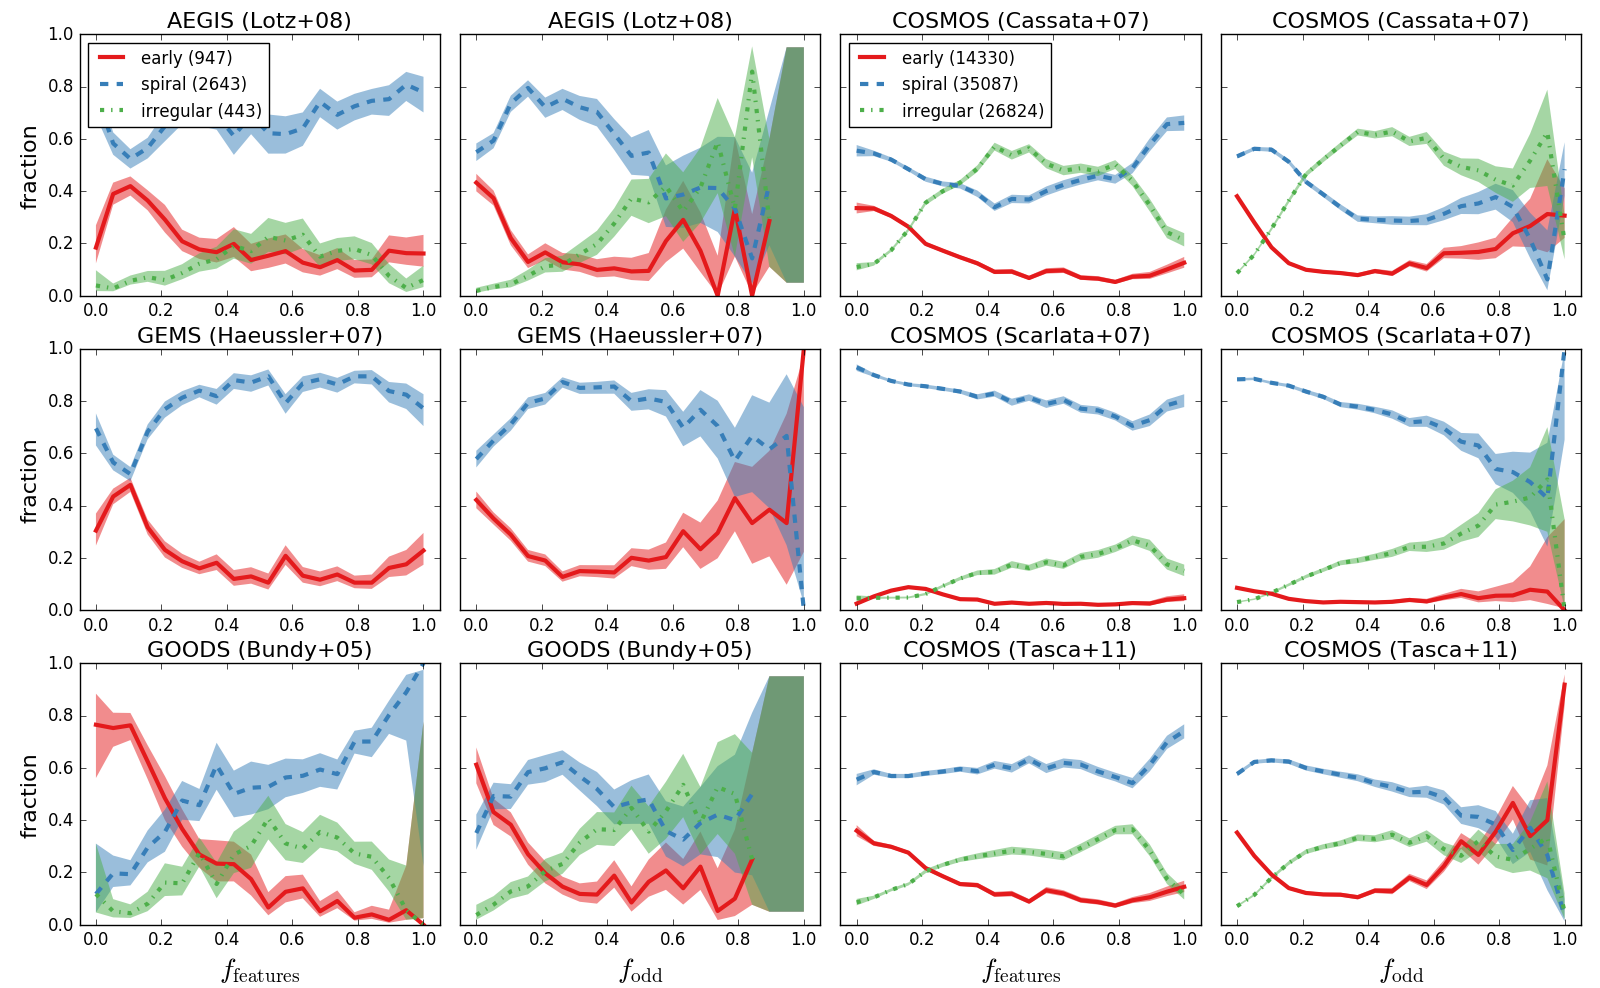
\includegraphics[width=1.0\textwidth]{figures/comparisons.png}
\caption{Distributions of morphological parameters for galaxies matched in GZH and other published catalogs, split by survey (AEGIS, COSMOS, GEMS, and GOODS). The first and third columns show the fraction of overall galaxies in the matched samples, split by their published morphologies as a function of the GZH \pbest. The corresponding second and fourth columns show data for the same galaxies as a function of \podd. Confidence intervals for each binned fraction in the bin are calculated for a binomial population \citep{cam11}.}
\label{fig:comparisons}
\end{figure*}

Figure~\ref{fig:comparisons} shows the proportion of galaxies as split by their automated/expert visual morphologies for each of the six catalogs matched to GZH. The relation between GZH and the automated/expert morphologies is shown to vary significantly for different surveys --- this may be due to intrisic differences in the galaxies, in the techniques used to measure morphology, or both. The distribution of \pbest{} for AEGIS galaxies is essentially flat for spirals, showing almost no difference in proportion at the highest and lowest ends. Early-type galaxies are at their highest proportion at \pbest$\sim0$, but constitute only 40\% of the galaxies at most. In contrast, GOODS galaxies at low \pbest{} are dominated by early-types, although spiral and irregular galaxies have comparable sizes as low as \pbest$\sim0.2$. In GEMS galaxies, the impact of irregular or peculiar galaxies is not measured; splitting on $n=2.5$ gives an essentially flat proportion of ellipticals to spirals at \pbest$>0.3$. Visual inspection of images of galaxies where both \pbest{} and $n$ are high show that the majority are obvious spirals but with prominent bulges, indicating that the single-component \sersic{} fit is likely choosing too small of an effective radius and missing the extended disk structure for a large population of galaxies. 

Even within the same sample of galaxies in COSMOS, different techniques of measuring morphology show significant differences. Both \citet{cas07} and \citet{tas11} have higher proportions of early-type galaxies at \pbest$\sim0$, but constitute less than half the sample in both cases. The majority of all galaxies in \citet{sca07}, in contrast, are spirals; oddly, the \emph{highest} proportions of spirals are found at the lowest values of \pbest. The decrease in spiral galaxies at higher \pbest{} is almost entirely balanced by an increase in irregulars. Early-types have a small bump near \pbest$\sim0.15$, but never constitute more than 10\% of the sample. 

The second set of plots in Figure~\ref{fig:comparisons} indicates that \podd{} is largely an effective method for separating irregular and/or peculiar galaxies from spirals. Despite the somewhat vague wording of the ``anything odd?'' question in GZH, the AEGIS, COSMOS, and GOODS all show a marked increase in the irregular fraction increasing with \podd. Any threshold value for distinguishing between the two, however, depends strongly on survey/redshift~range. 

As the data shown in Figure~\ref{fig:comparisons} cover a wide range of redshifts and sizes, a volume-limited sample of galaxies (or at least binning by redshift) is likely a much more appropriate comparison. While we leave detailed analysis to a further paper, we note that there is no strong change in the proportion of galaxies when binning by redshift intervals of $\Delta z=0.2$ out to $z=1.0$. 

\section{Summary}\label{sec:summary}

%Now people go and do science with these awesome GZH classifications. 

This paper presents the catalog release for the Galaxy Zoo: Hubble project, which uses crowdsourced visual classifications to measure galaxy morphologies. The first two phases of Galaxy Zoo \citep{lin11,wil13} used images of low-redshift galaxies from SDSS; this is the first phase of the project with space-based images of high-redshift targets (in addition to the Galaxy Zoo: CANDELS collaboration; Simmons et al., submitted). The final sample includes classifications for 181,101~images generated from 150,771~unique galaxies. Galaxies were selected from a brightness-limited sample from multiple Legacy surveys using the Advanced Camera for Surveys on the Hubble Space Telescope, including AEGIS, GEMS, GOODS-N, GOODS-S, and COSMOS. We also include classifications for 51,861 Sloan Digital Sky Survey images in Stripe~82 at relatively low redshift; these serve both as a low-redshift anchor for cosmological studies and a potential comparison for the different epochs of classification between GZH and Galaxy Zoo 2 \citep{wil13}. 

The data for the GZH catalogs has been extensively tested and reduced. The dominant effect is a known bias against identifying disky and asymmetric sub-structures at either low resolution or surface brightness. This can be the result either of genuinely small or dim galaxies, or a perceived effect from observing galaxies at further distances (higher redshift). To calibrate this \emph{without} potentially overcorrecting for the genuine morphological evolution of galaxies over cosmic time, we use SDSS images of low-redshift galaxies, process them to appear as if they were at higher redshift, and pass them through the GZH interface in an identical fashion. The resulting change in \pfeatures{} as a function of $z$,$\mu$ is applied as a multiplicative correction to the top-level vote fractions for $\sim50\%$ of the GZH galaxies. 

Galaxies in GZH show significant changes in the disk/elliptical fraction as a function of redshift, along with an increasing number of galaxies dominated by smaller clumps and presumed to be in the process of building up their baryonic mass through a combination of hierarchical merging and in-situ star formation. While the majority of scientific interpretation is left to future papers, we confirm the decrease in observed bar fraction with increasing redshift \citep{mel14} and identify a new way for identifying clumpy galaxies as a function of clump multiplicity.

The full data tables for the catalogs can be accessed in machine-readable form from both the journal and at \url{http://data.galaxyzoo.org}.
 
\acknowledgments

We thank Meg Schwamb and the ASIAA for hosting the ``Citizen Science in Astronomy'' workshop, 3-7 Mar 2014 in Taipei, Taiwan, at which some of this analysis was done. We also thank Jennifer Lotz for sharing her $G$-$M_{20}$ measurements for the AEGIS sample.

This project made heavy use of the Astropy packages in Python \citep{ast13}, the \texttt{seaborn} plotting package \citep{was15}, and astroML \citep{van12}. Modified code from Nick~Wherry and David~Schlegel was used to create the JPG images. 

This work is based on (GO-10134, GO-09822, GO-09425.01, GO-09583.01, GO-9500) program observations with the NASA/ESA Hubble Space Telescope, obtained at the Space Telescope Science Institute, which is operated by the Association of Universities for Research in Astronomy, Inc., under NASA contract NAS 5-26555. 

Funding for the SDSS and SDSS-II has been provided by the Alfred P. Sloan Foundation, the Participating Institutions, the National Science Foundation, the U.S. Department of Energy, the National Aeronautics and Space Administration, the Japanese Monbukagakusho, the Max Planck Society, and the Higher Education Funding Council for England. The SDSS website is \url{http://www.sdss.org/}. 

The SDSS is managed by the Astrophysical Research Consortium for the Participating Institutions. The Participating Institutions are the American Museum of Natural History, Astrophysical Institute Potsdam, University of Basel, University of Cambridge, Case Western Reserve University, University of Chicago, Drexel University, Fermilab, the Institute for Advanced Study, the Japan Participation Group, Johns Hopkins University, the Joint Institute for Nuclear Astrophysics, the Kavli Institute for Particle Astrophysics and Cosmology, the Korean Scientist Group, the Chinese Academy of Sciences (LAMOST), Los Alamos National Laboratory, the Max-Planck-Institute for Astronomy (MPIA), the Max-Planck-Institute for Astrophysics (MPA), New Mexico State University, Ohio State University, University of Pittsburgh, University of Portsmouth, Princeton University, the United States Naval Observatory and the University of Washington. 

\bibliography{gz_hubble_data}

\newpage
\clearpage

\appendix

\section{GOODS Shallow Depth data}


\begin{table}
\caption{Correctable fractions for the top-level task in GZH in the GOODS shallow-depth (2-epoch) images. \label{tbl:goods_shallow_categories}}
\begin{tabular}{lrrrrrrrr}
\hline\hline
                                   & GOODS-N & GOODS-S & Total \\
\hline
Correctable                        & 748     & 514     & 1,262 \\
Lower limit                        & 526     & 1,143   & 1,669 \\
No Correction Needed ($z \le 0.3$) & 267     & 267     & 534   \\ 
NEI                                & 851     & 2,670   & 3,521 \\
No Redshift Information            & 159     & 319     & 478   \\
Total                              & 2,551   & 4,913   & 7,464 \\
\hline\hline
\end{tabular}
\end{table}



GZH used both 5-epoch and 2-epoch sets of data to construct the GOODS set of images. The 11,157 full depth 5-epoch images are used in the main catalog; the classifications for the 7,464 shallow depth 2-epoch images are offered as a supplementary table. Here we briefly analyze the effect of image depth on the ability of the GZ users to identify features or disk structure in the images. 

\subsection{Comparing shallow and full depth morphologies}

Of the 11,157 galaxies in the GOODS-N and GOODS-S full depth sample, 4,461 of these are in the shallow-depth sample. Figure~\ref{fig:shallow_vs_full} shows a strong correlation between $\rm p_{features}$ for both sets of images. The mean change in $\rm p_{features}$ from the shallow to full depth images  $\rm p_{features,full} - p_{features,shallow} \equiv \Delta p = 0.00$, with a standard deviation of $\sigma = 0.17$. While there is some variance in $\Delta p$ in the whole sample, the change is usually small and not often significant enough to change a morphological classification. Defining a clean sample of disk galaxies as those with $p_{features,best}>0.8$, elliptical galaxies as those with  $p_{smooth,best}<0.2$, and intermediate as those in between, 75\% of the sample would not change morphology. Of the remaining 25\% that would change morphology, only 0.3\% (representing 10 galaxies total) drastically change morphology from smooth to featured or visa versa, while the rest would transition to or from the ``intermediate'' morphology. Details can be seen in Table~\ref{tbl:shallow_to_full_stats} and examples of images representing the 9 possible changes (or lack of) in morphology are shown in Figures~\ref{fig:shallow_smooth},\ref{fig:shallow_intermediate}, and \ref{fig:shallow_featured}.

\begin{figure}
\begin{center}
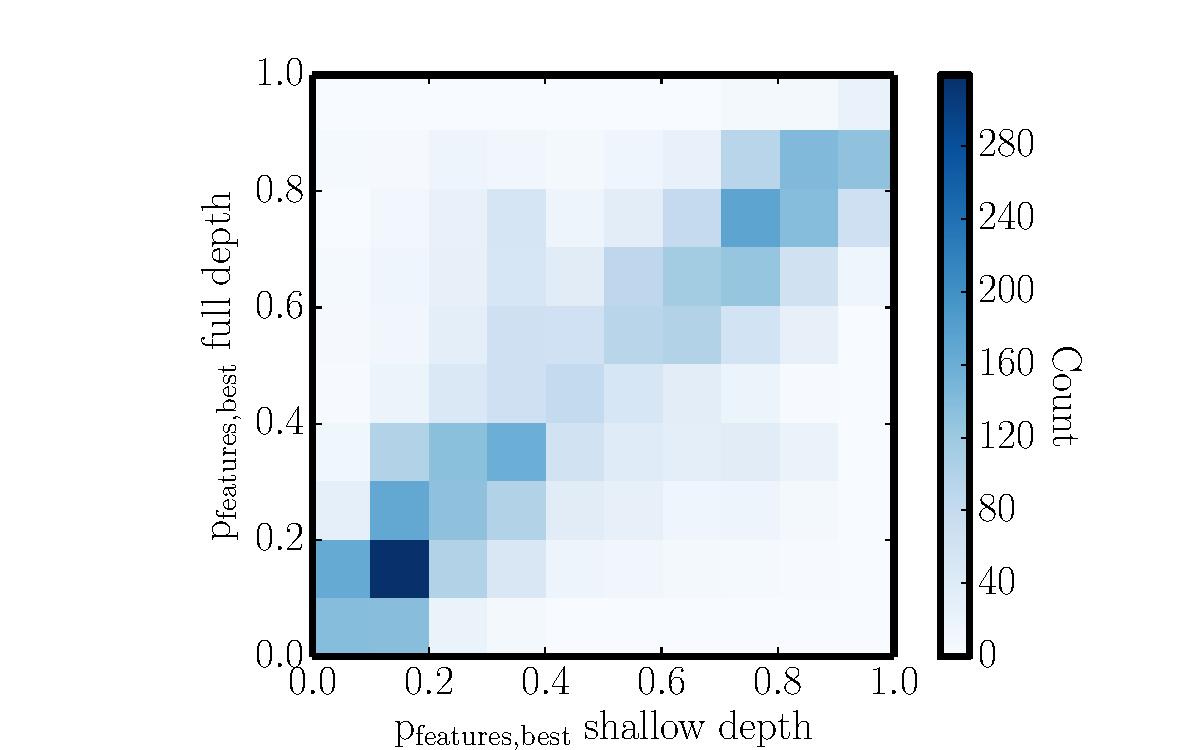
\includegraphics[width=0.50\textwidth]{figures/full_shallow_p_plot.pdf}
\caption{shallowfull}
\label{fig:shallow_vs_full}
\end{center}
\end{figure}

\begin{table}
\caption{Properties of galaxies whose morphologies changed or stayed the same in the shallow vs full images. Featured here is defined as $p_{features,best}>0.8$, intermediate = $0.2<p_{features,best}<0.8$, smooth = $p_{smooth,best}<0.2$. \label{tbl:shallow_to_full_stats}}
\begin{tabular}{lrrrrrrrr}
\hline\hline
shallow to full morphology    & N       & \%       & $<\Delta p>$ & $<z>$ \\
\hline
smooth to smooth              & 758     & 17.0     & -0.00        &  0.69\\
smooth to intermediate        & 367     & 8.2      & 0.18         &  0.69\\
smooth to featured            & 7       & 0.2      & 0.76         &  0.57\\ 
intermediate to smooth        & 214     & 4.8      & -0.18        &  0.65\\
intermediate to intermediate  & 2,303   & 51.6     & 0.01         &  0.78 \\
intermediate to featured      & 168     & 3.8      & 0.19         &  0.83\\
featured to smooth            & 3       & 0.1      & -0.74        &  0.71\\
featured to intermediate      & 337     & 7.6      & -0.18        &  0.68\\
featured to featured          & 301     & 6.8      & -0.05        &  0.71\\

Total                         & 4,461   & 100      &              & \\
\hline\hline
\end{tabular}
\end{table}



\begin{figure*}
\centering

\subfigure{[a]\label{fig:smooth_to_smooth}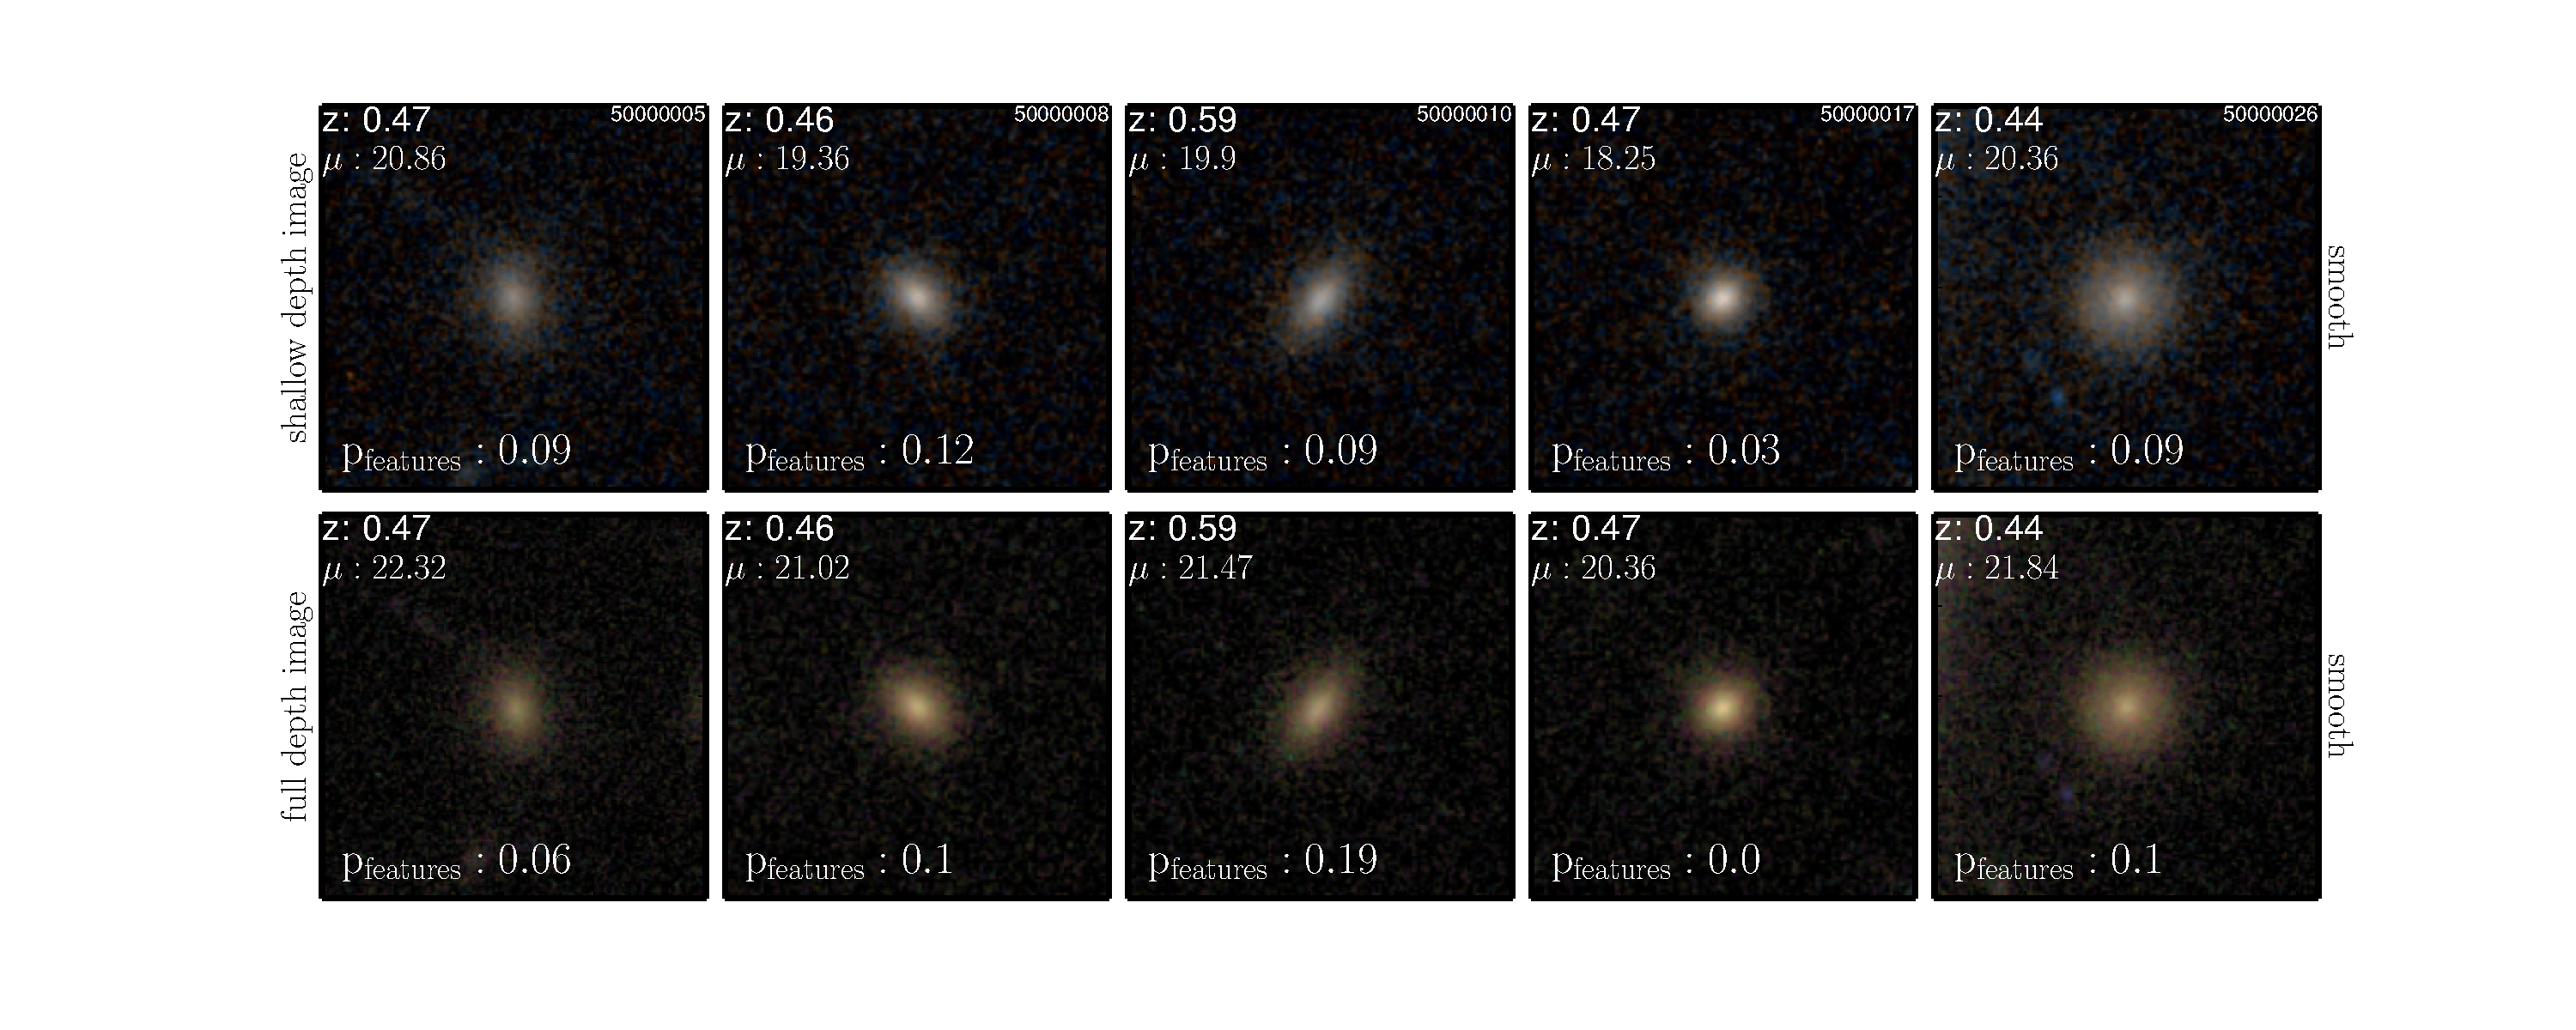
\includegraphics[width=\textwidth]{figures/smooth_to_smooth.pdf}}

\subfigure{[b]\label{fig:smooth_to_int}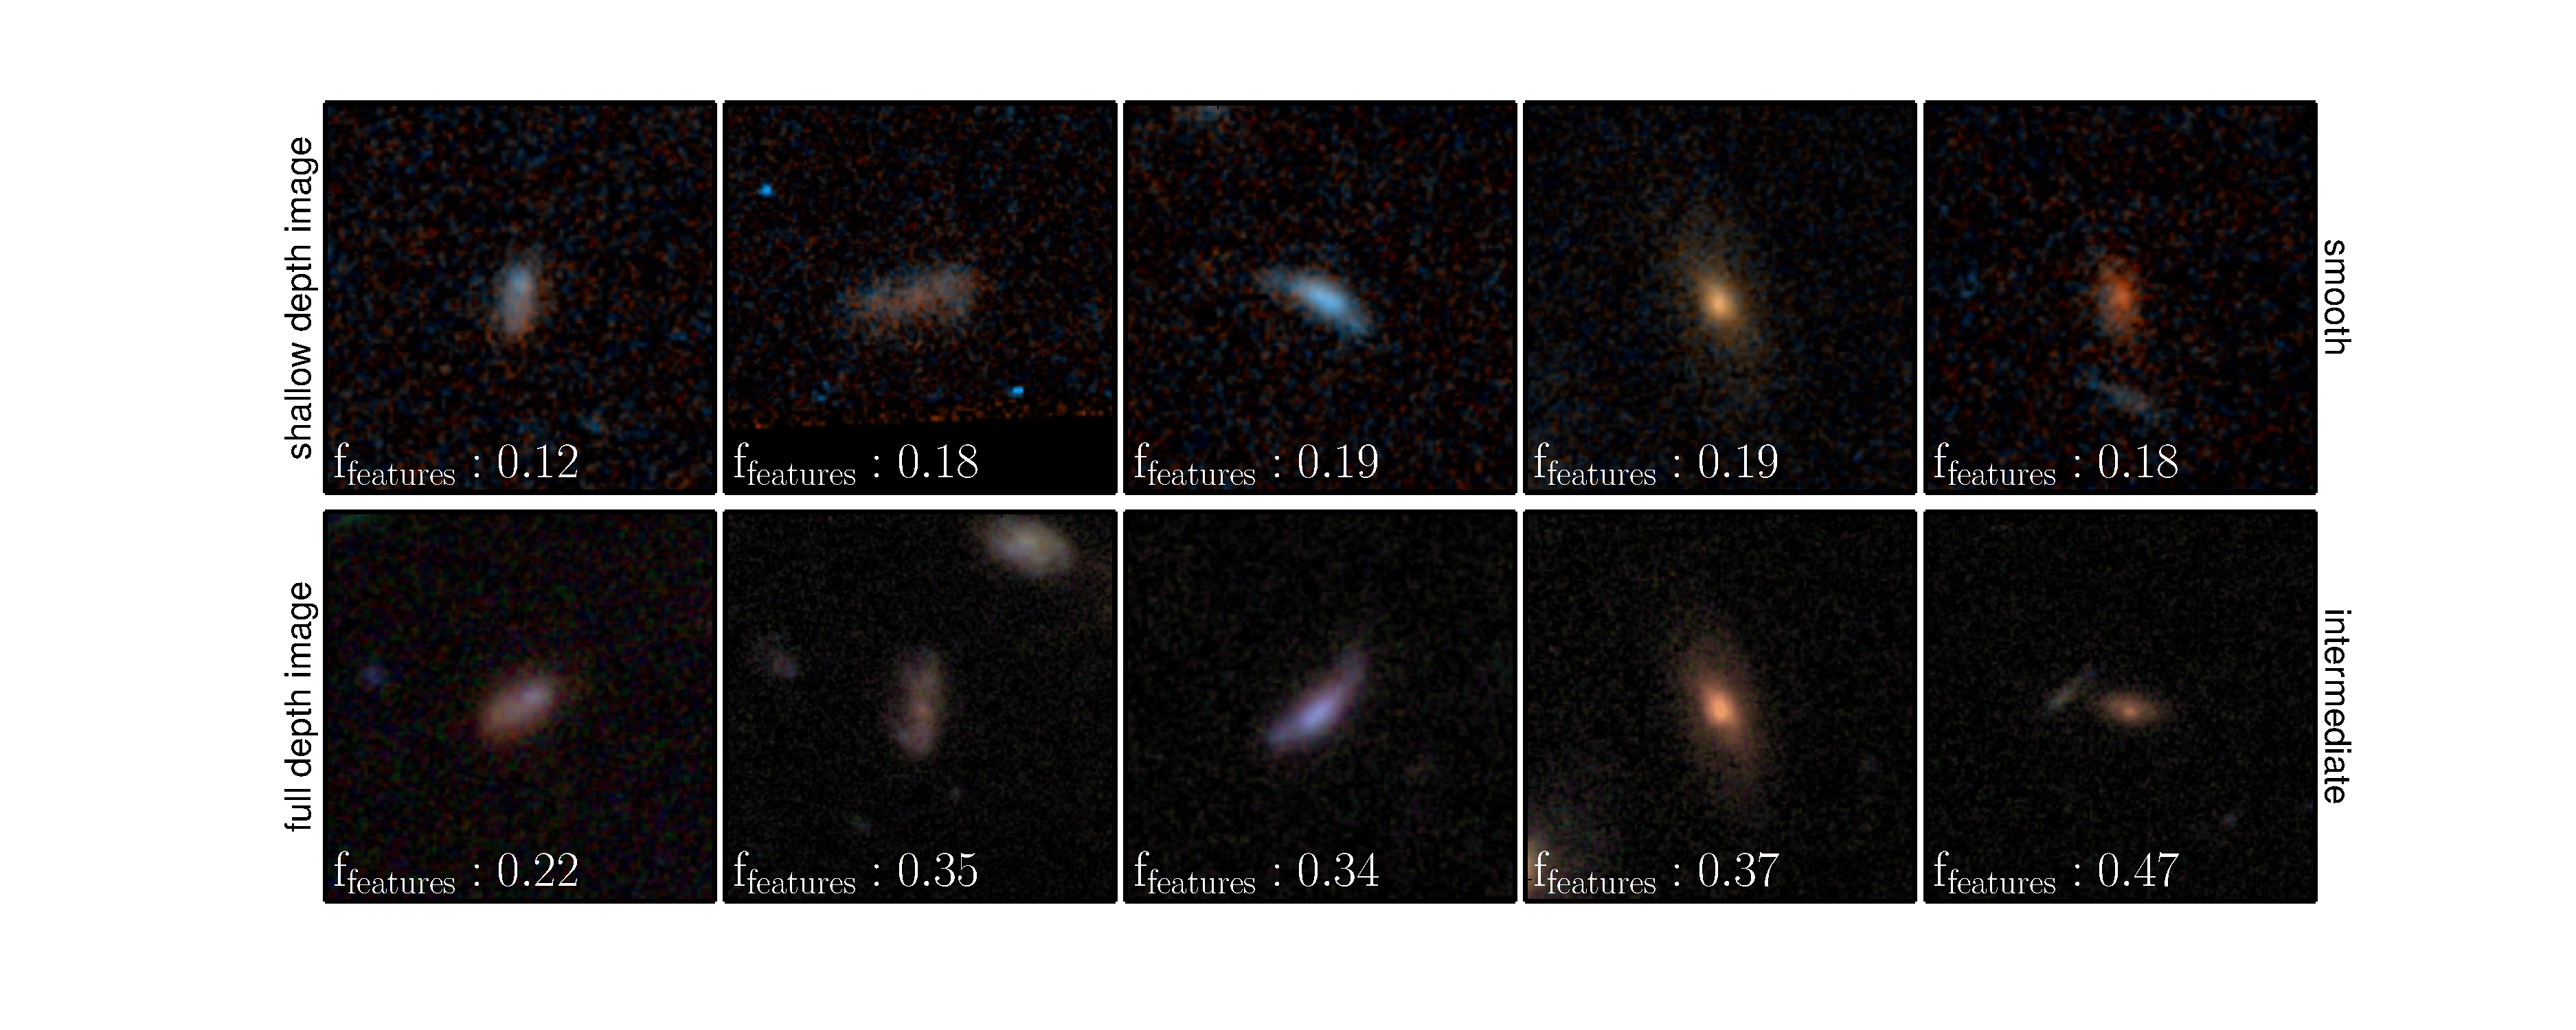
\includegraphics[width=\textwidth]{figures/smooth_to_intermediate.pdf}}

\subfigure{[c]\label{fig:smooth_to_featured}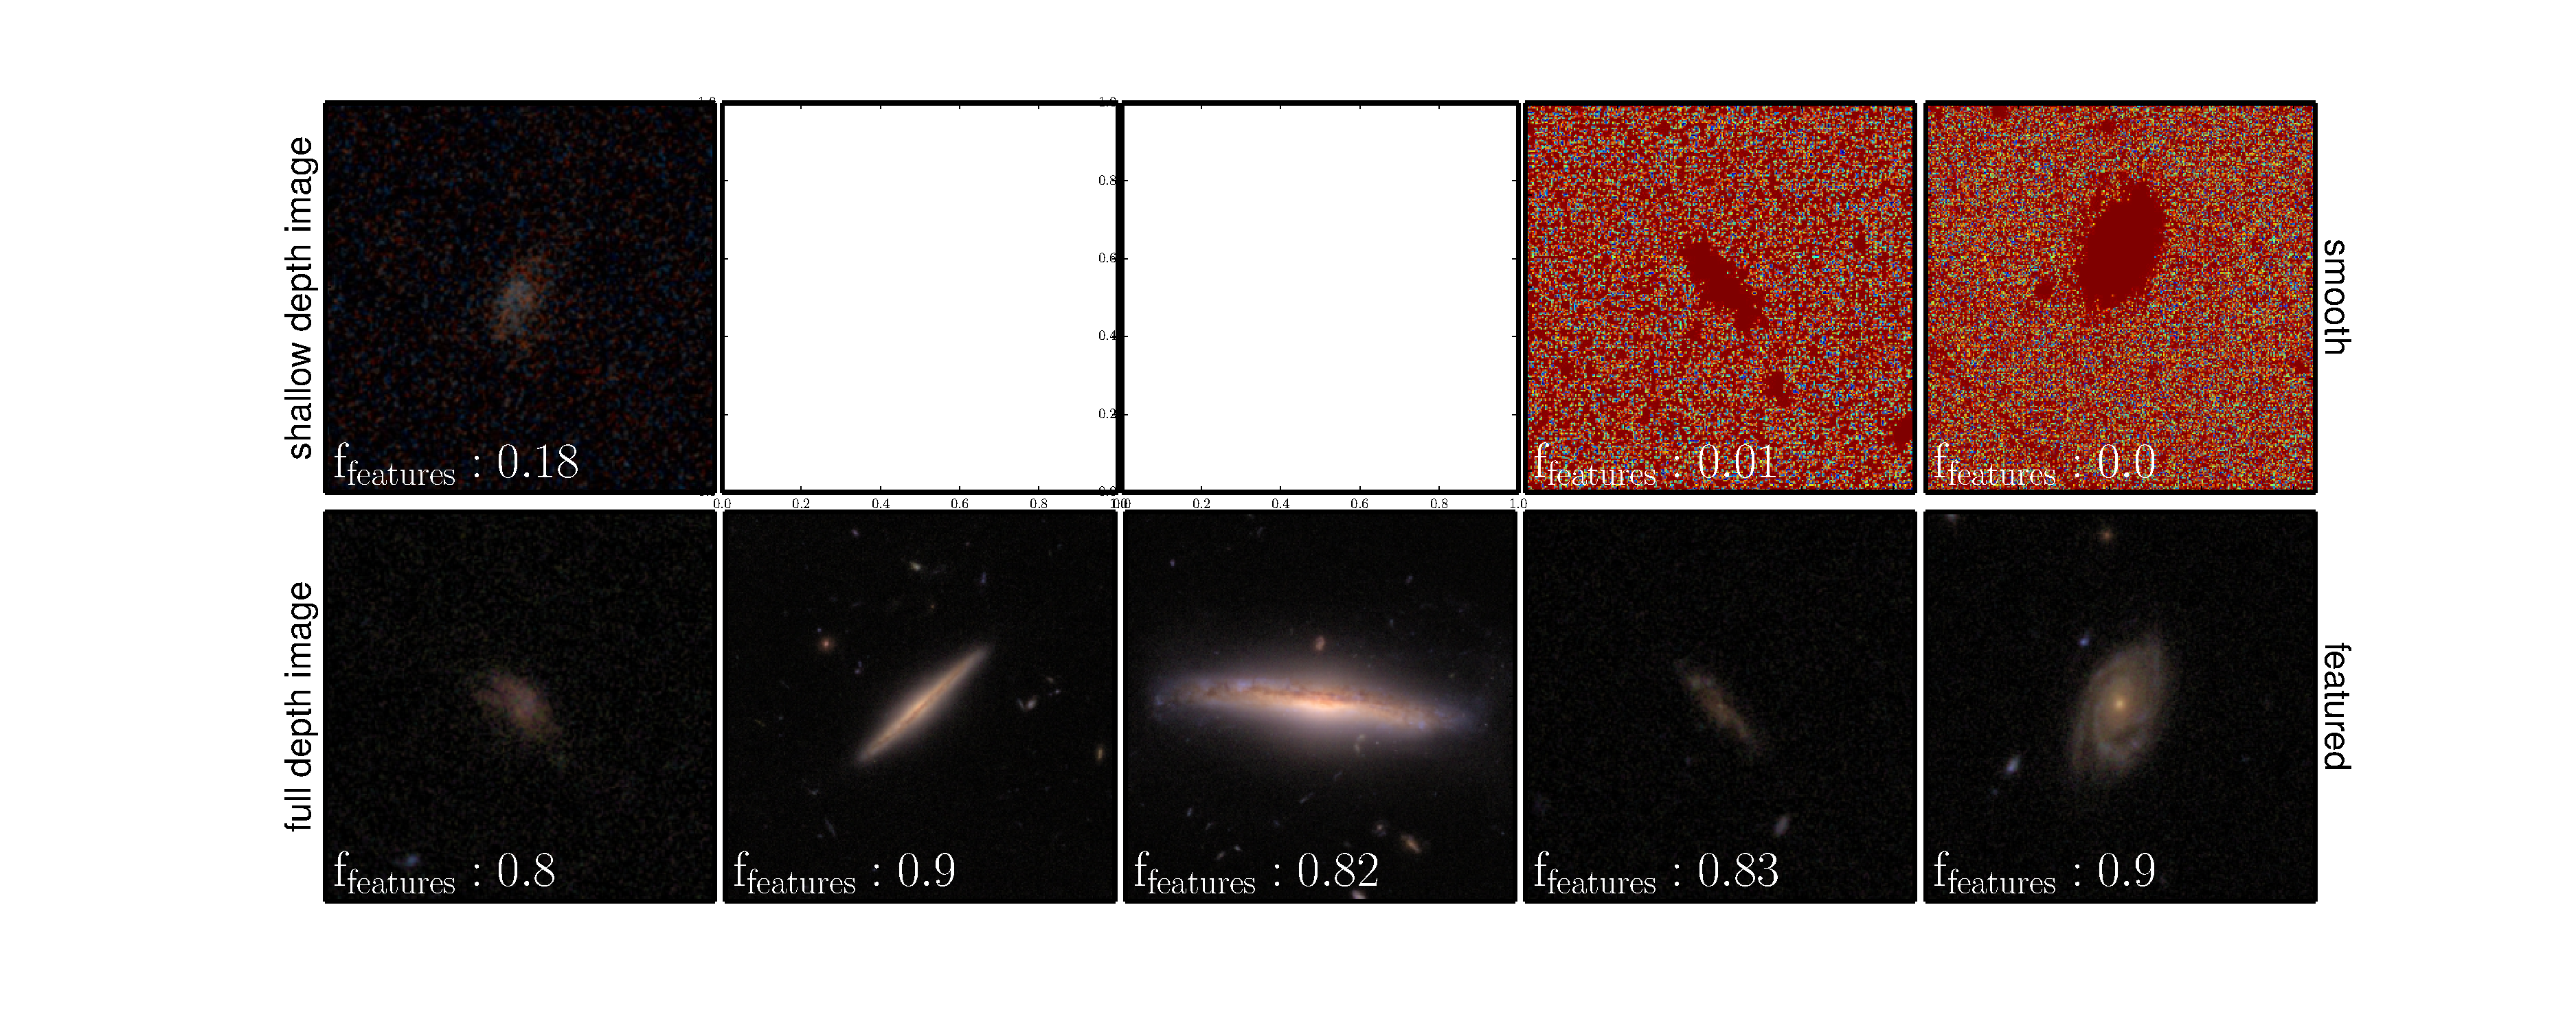
\includegraphics[width=\textwidth]{figures/smooth_to_featured.pdf}}

\caption{Galaxies whose shallow images were classified as smooth and full depth images were classified as smooth, intermediate, or featured.}
\label{fig:shallow_smooth}
\end{figure*}

\begin{figure*}
\centering

\subfigure{[b]\label{fig:int_to_smooth}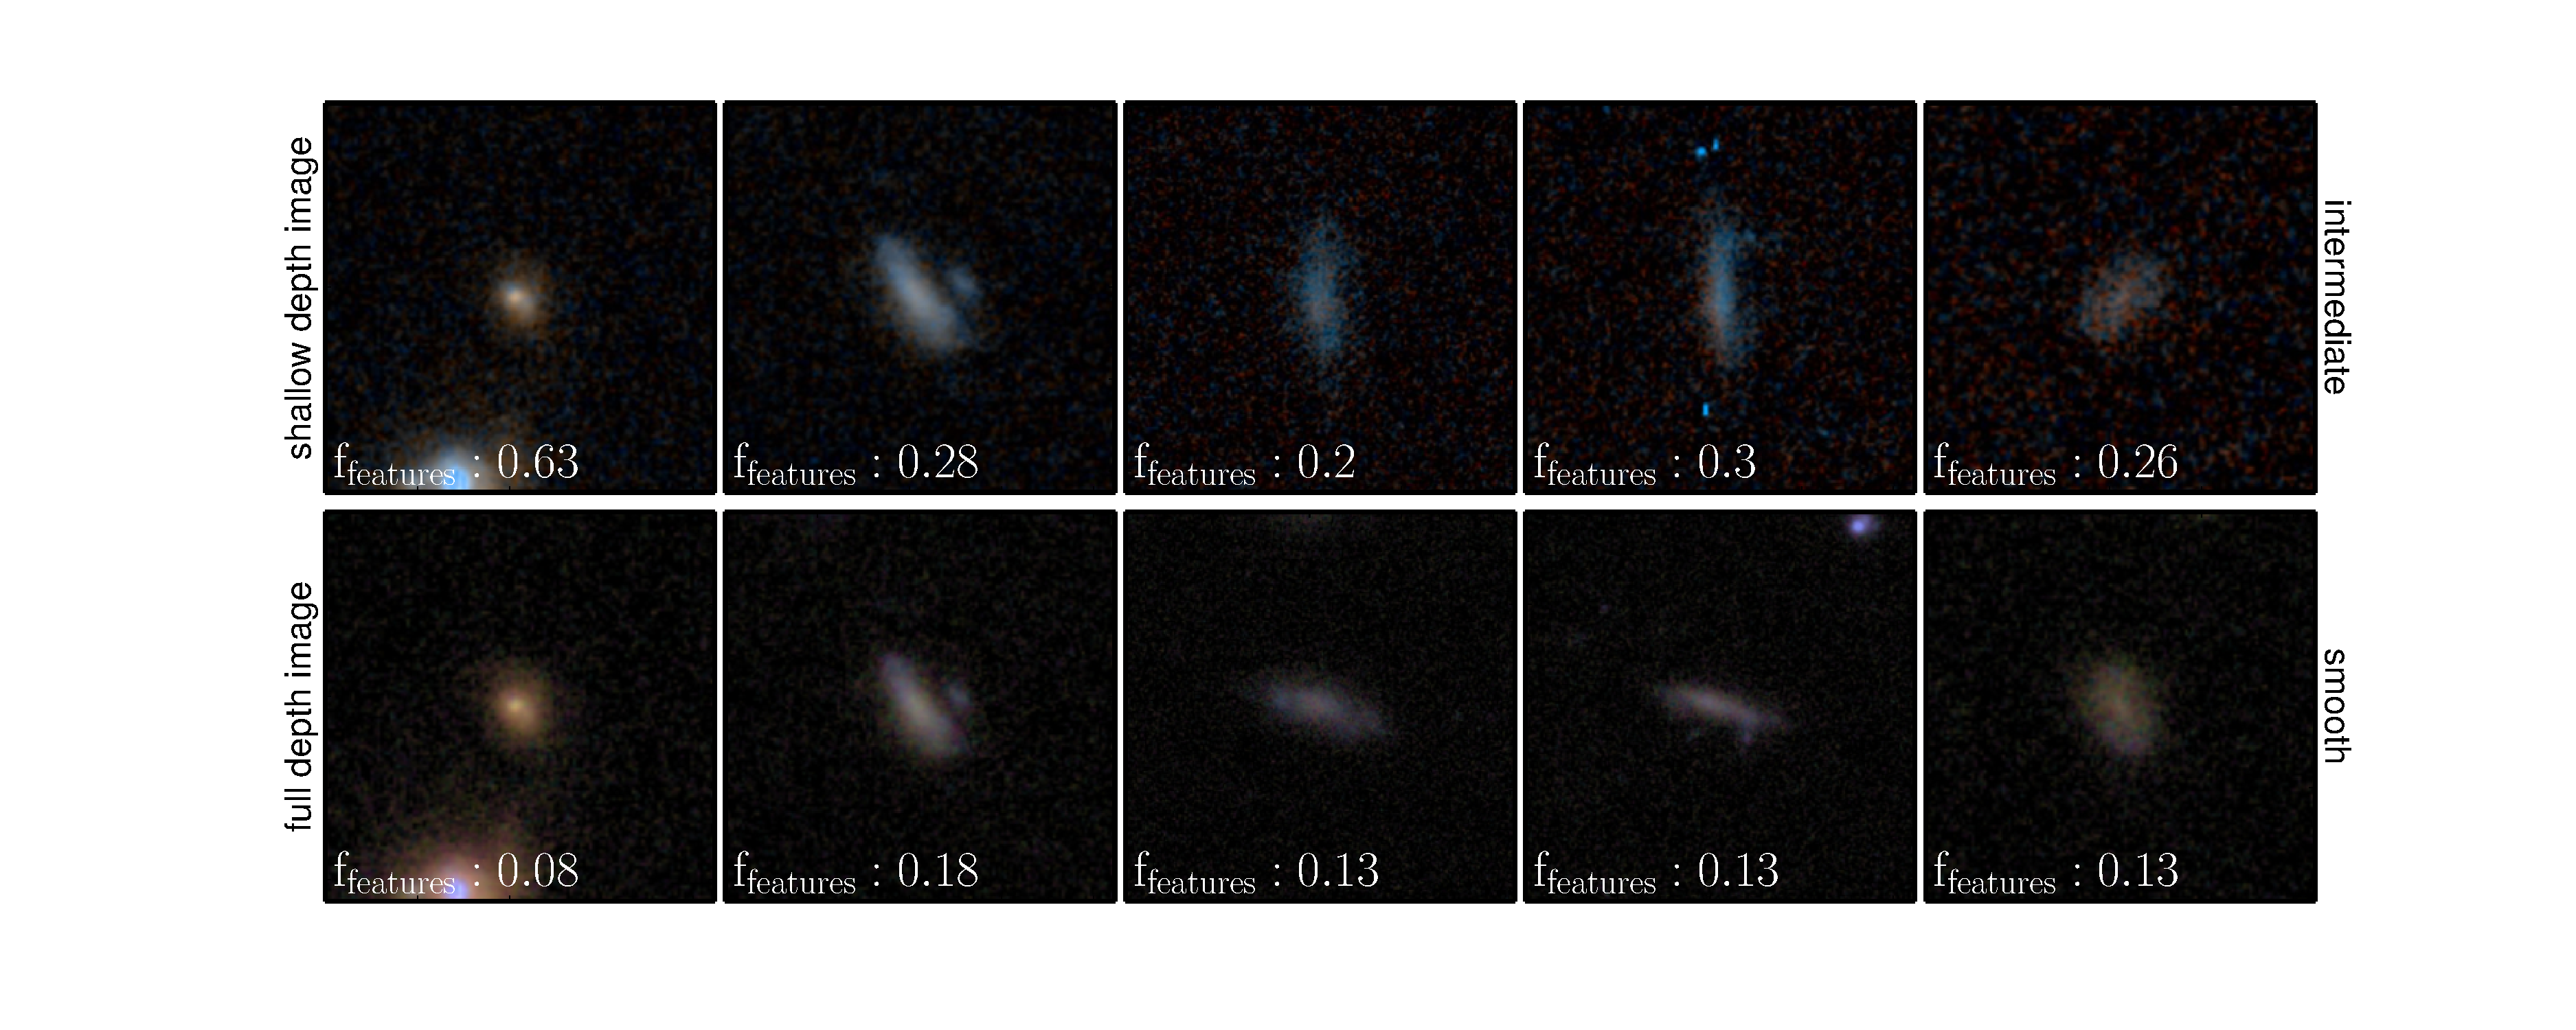
\includegraphics[width=\textwidth]{figures/intermediate_to_smooth.pdf}}

\subfigure{[b]\label{fig:int_to_int}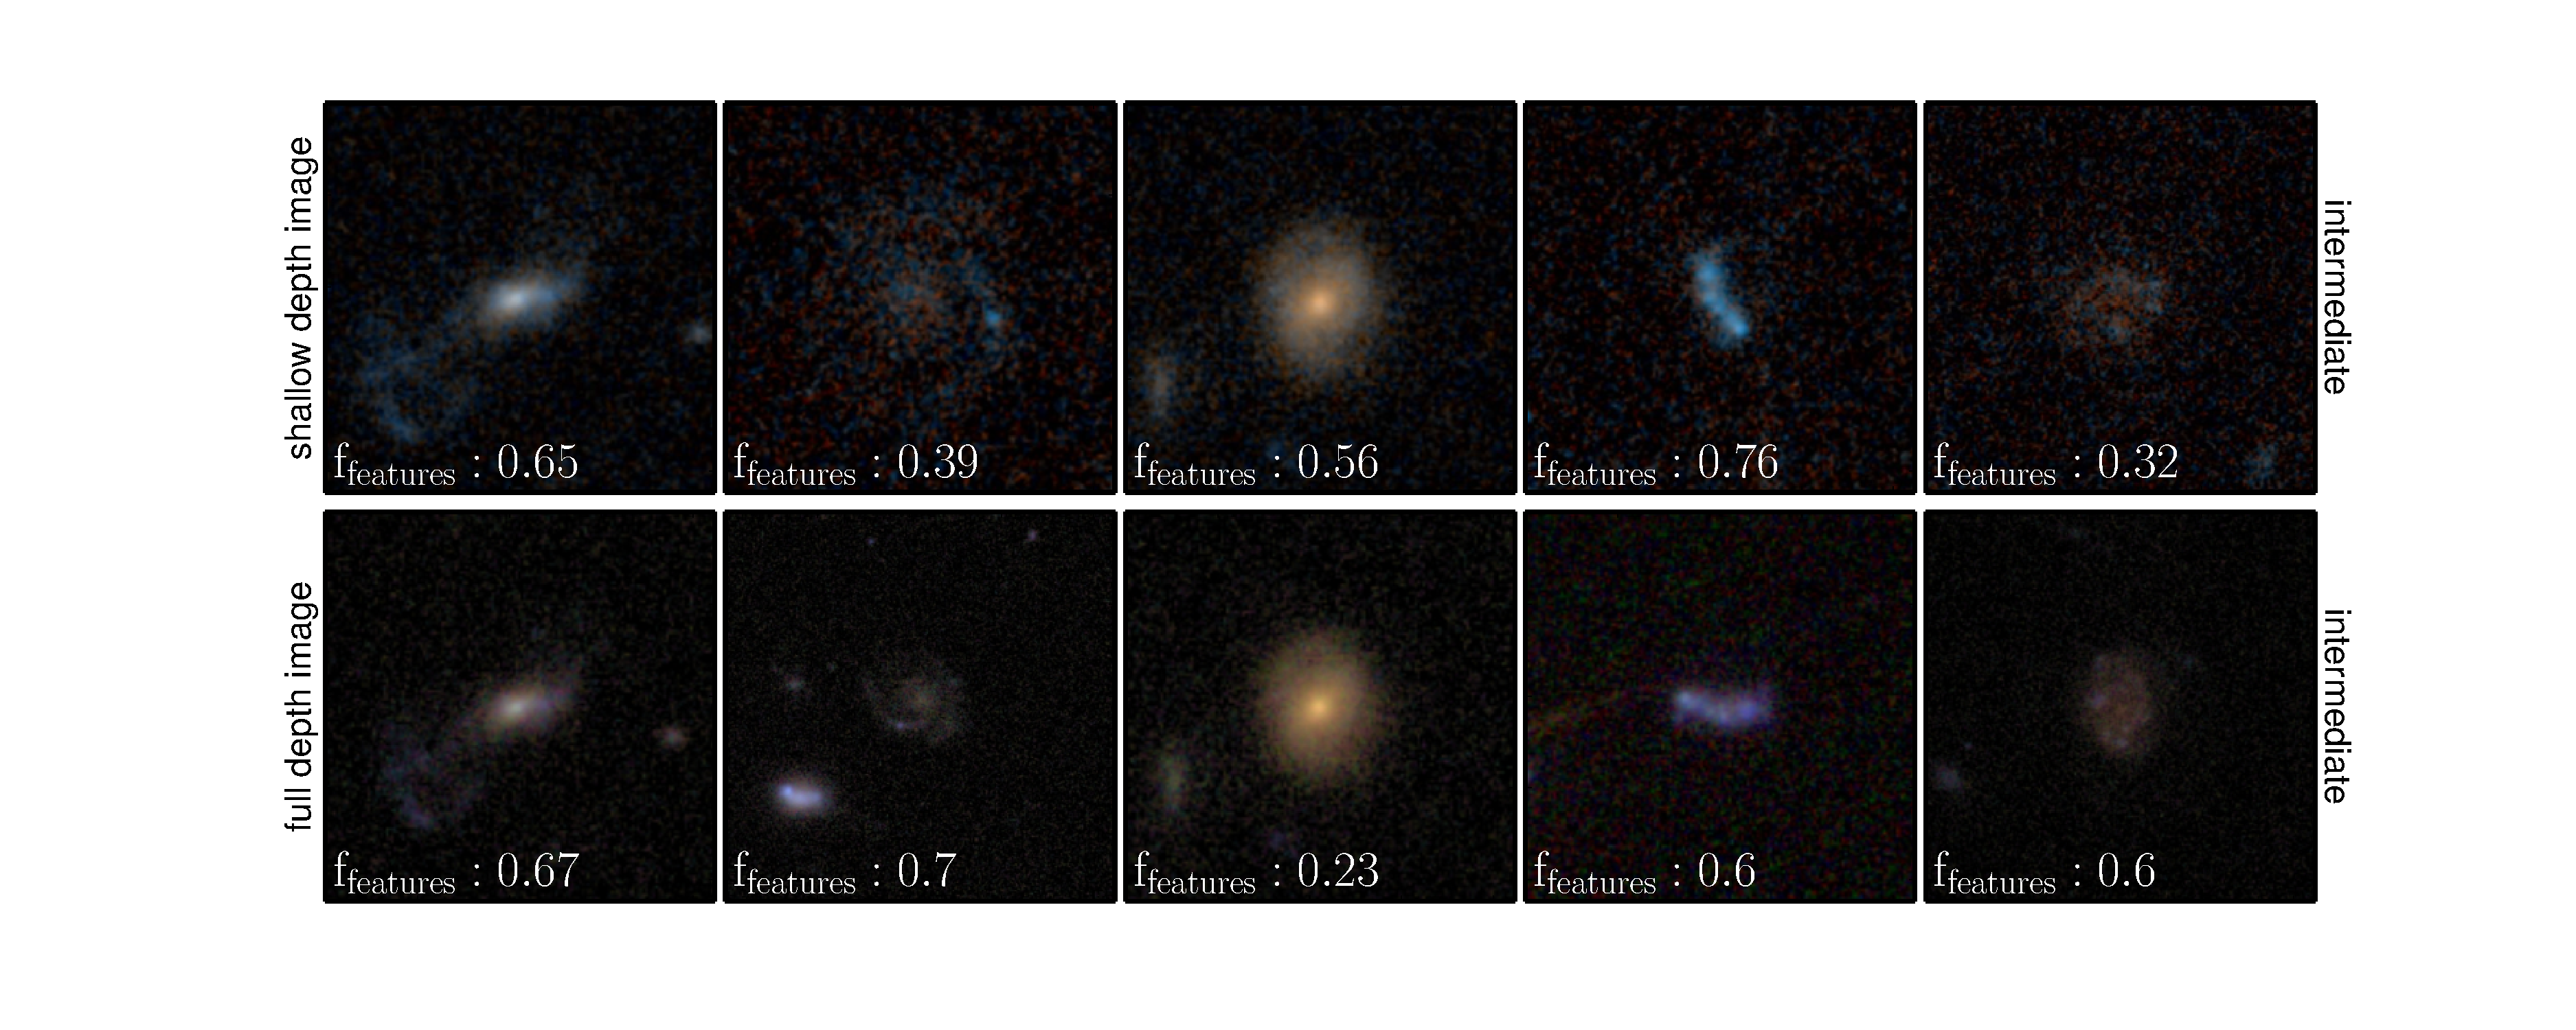
\includegraphics[width=\textwidth]{figures/intermediate_to_intermediate.pdf}}

\subfigure{[b]\label{fig:int_to_featured}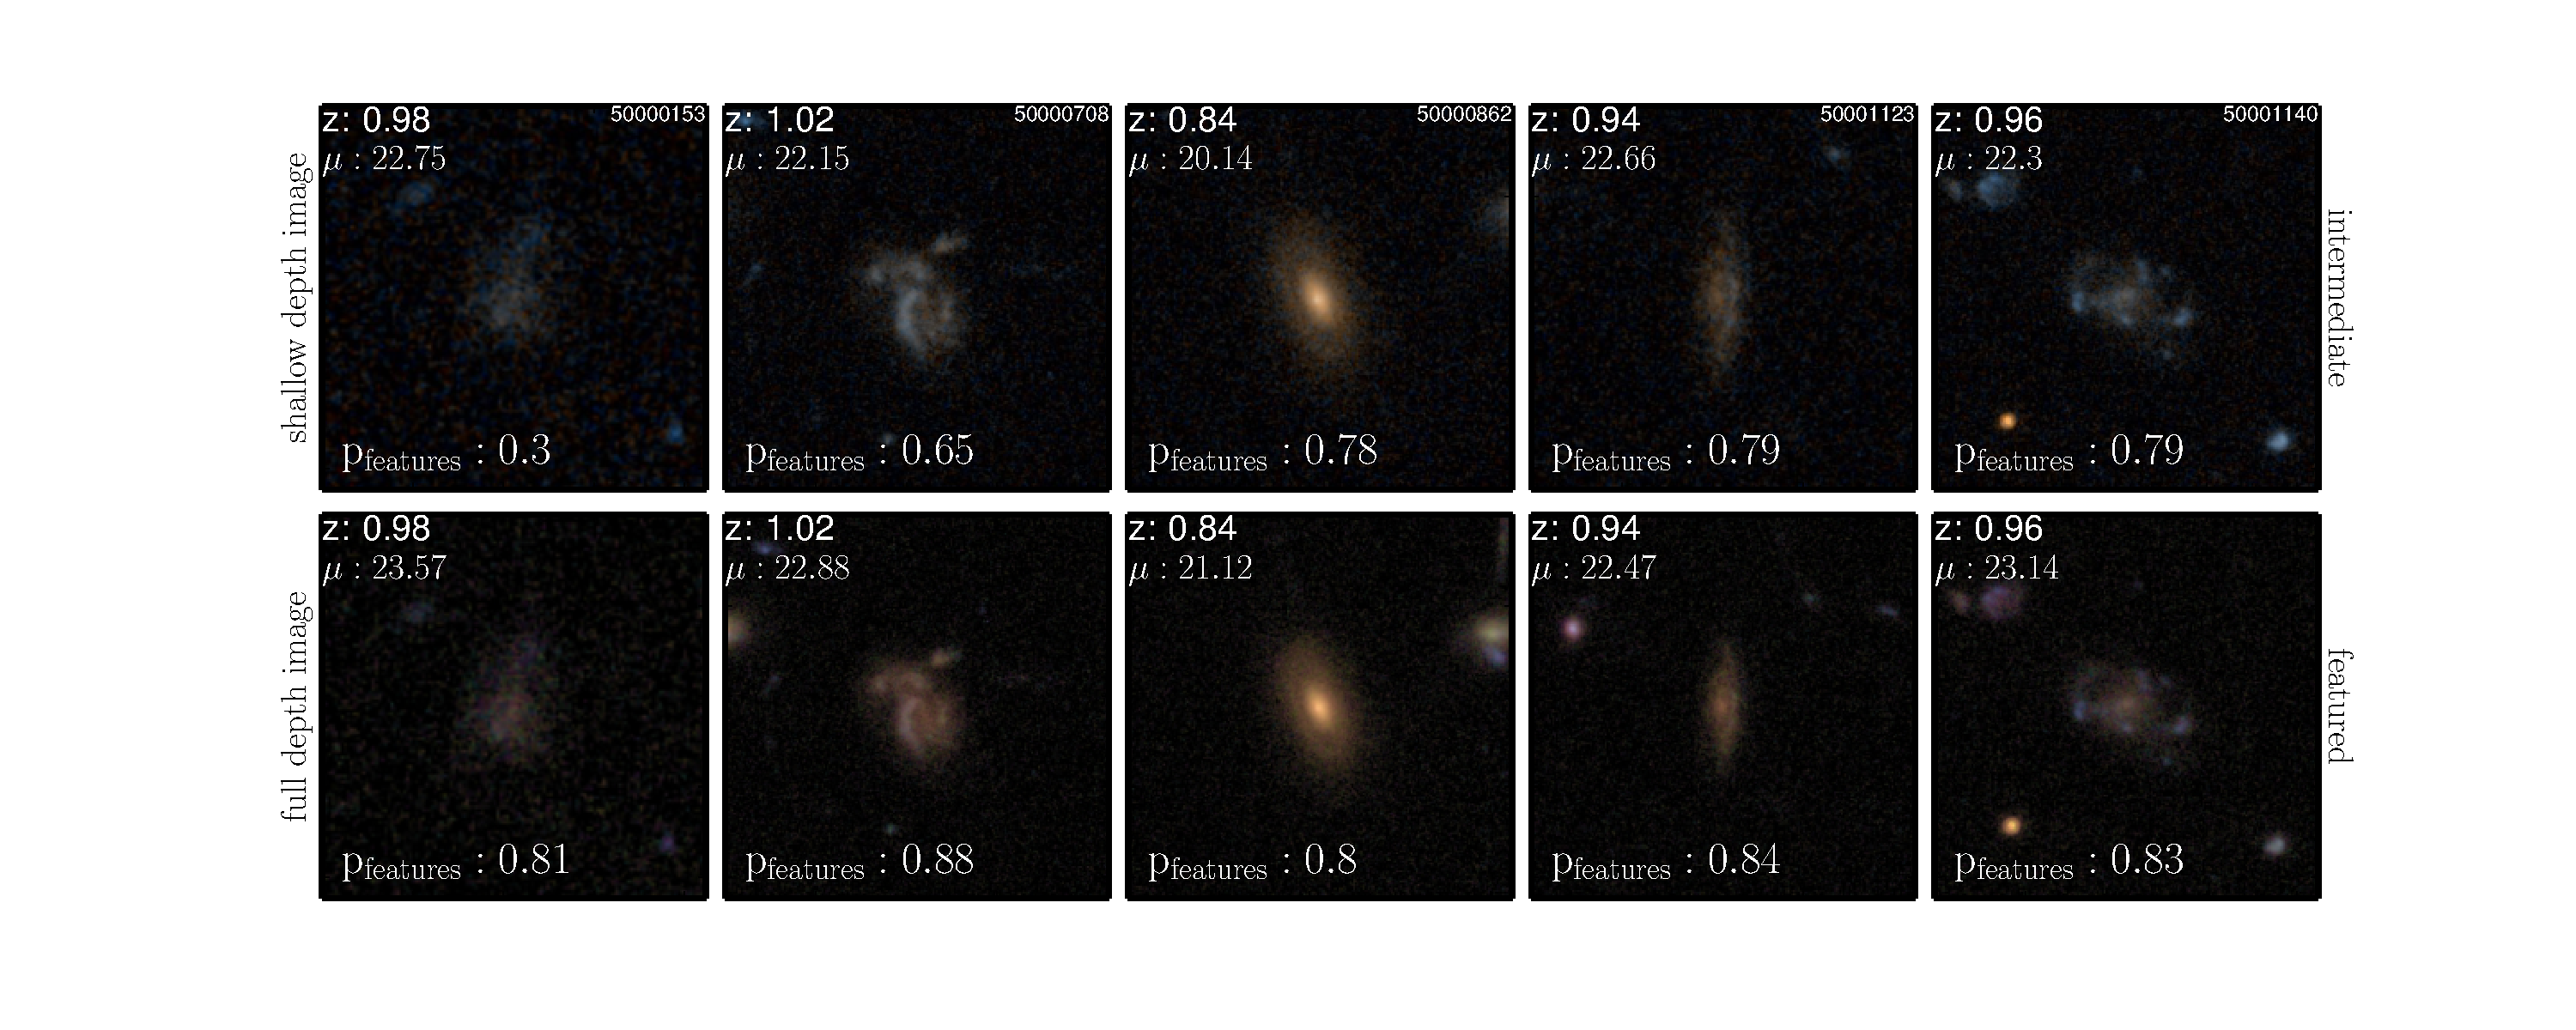
\includegraphics[width=\textwidth]{figures/intermediate_to_featured.pdf}}

\caption{Galaxies whose shallow images were classified as intermediate and full depth images were classified as smooth, intermediate, or featured.}
\label{fig:shallow_intermediate}
\end{figure*}

\begin{figure*}
\centering

\subfigure{[b]\label{fig:featured_to_smooth}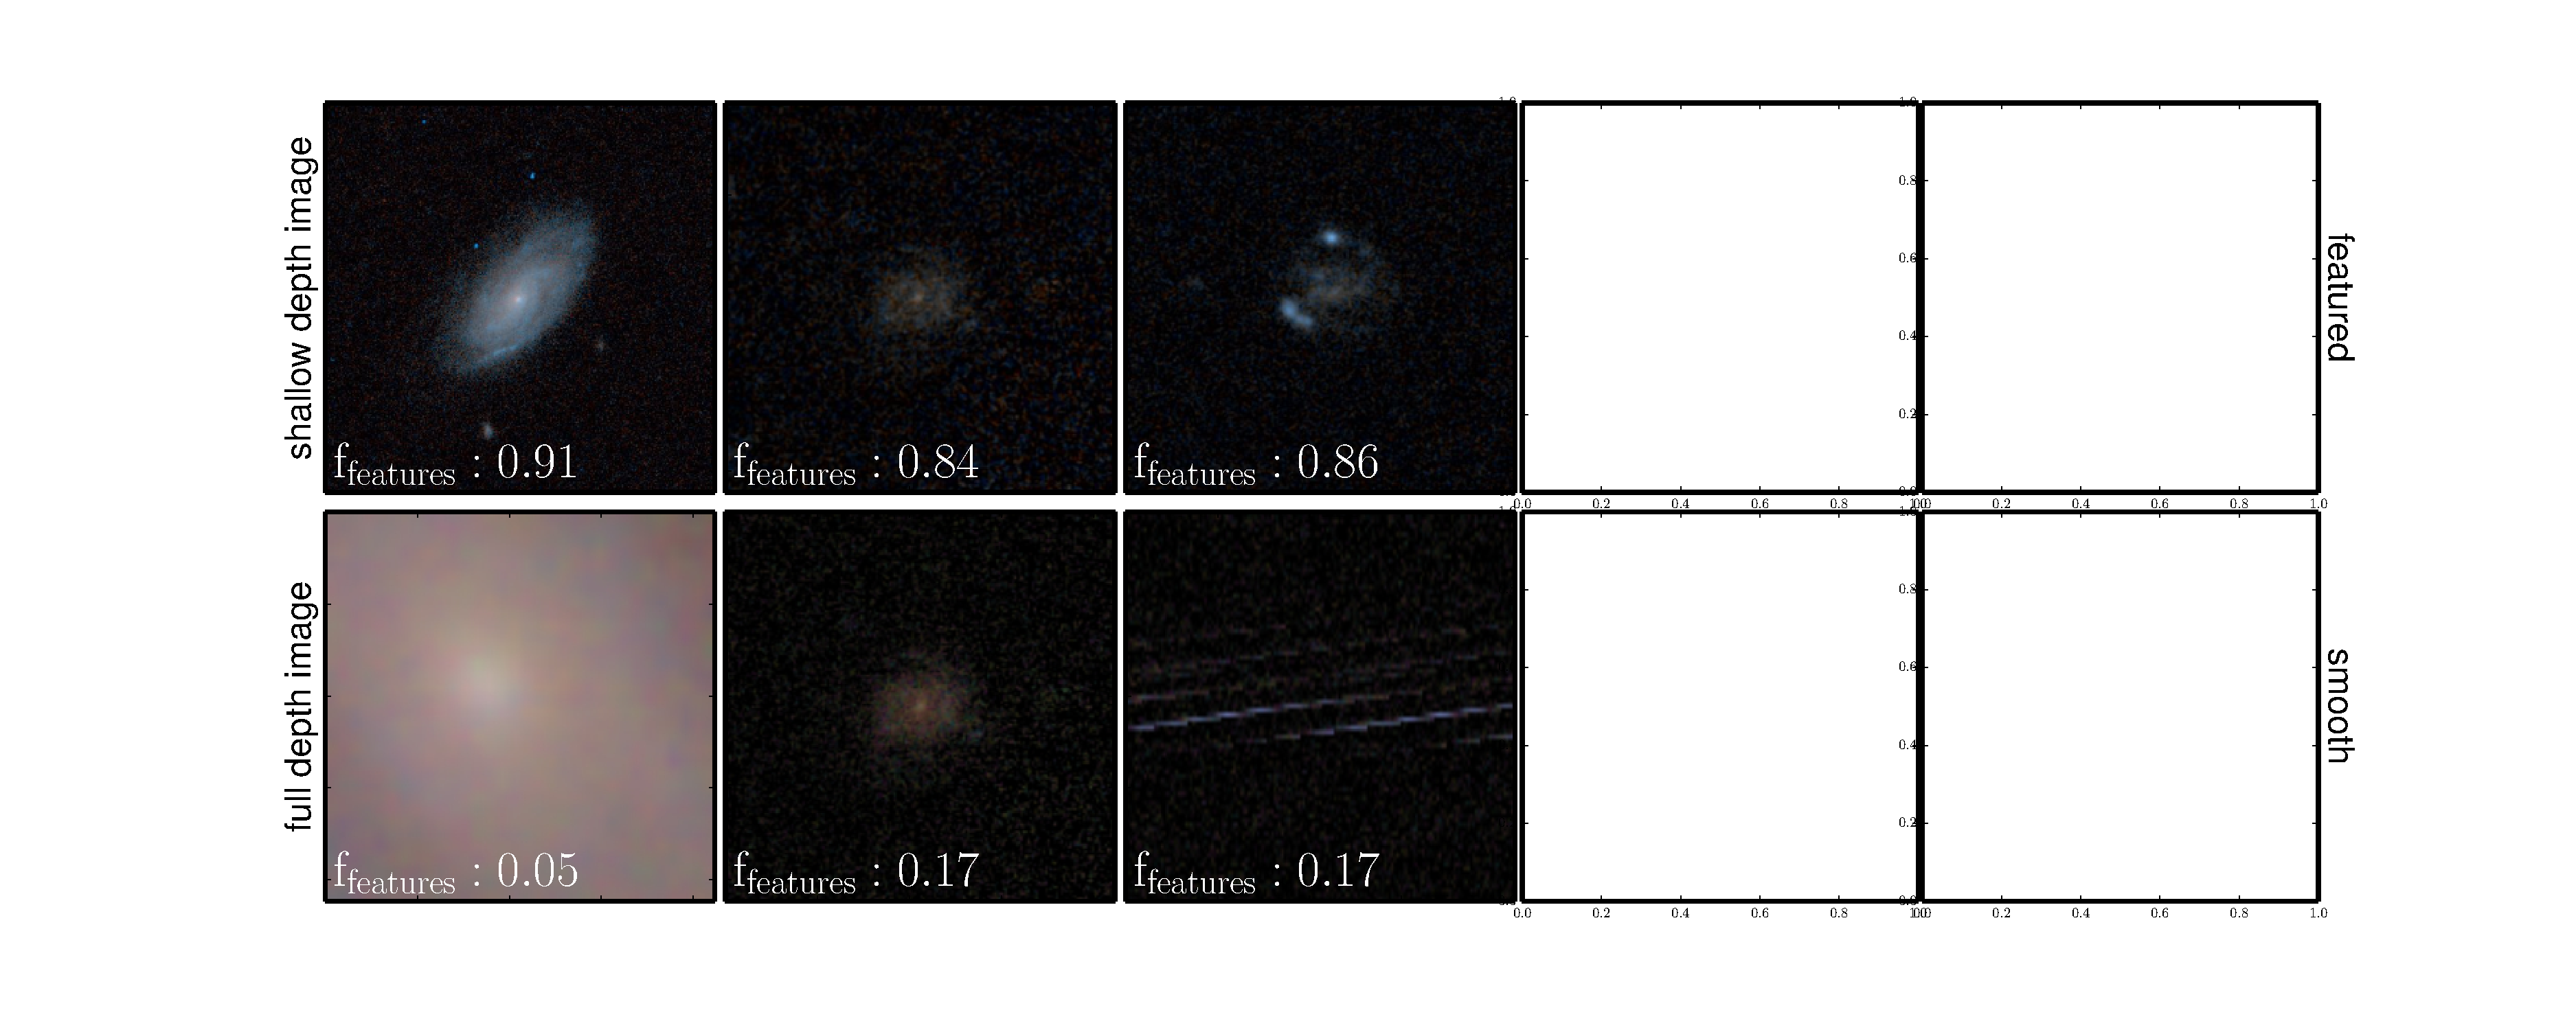
\includegraphics[width=\textwidth]{figures/featured_to_smooth.pdf}}

\subfigure{[b]\label{fig:featured_to_int}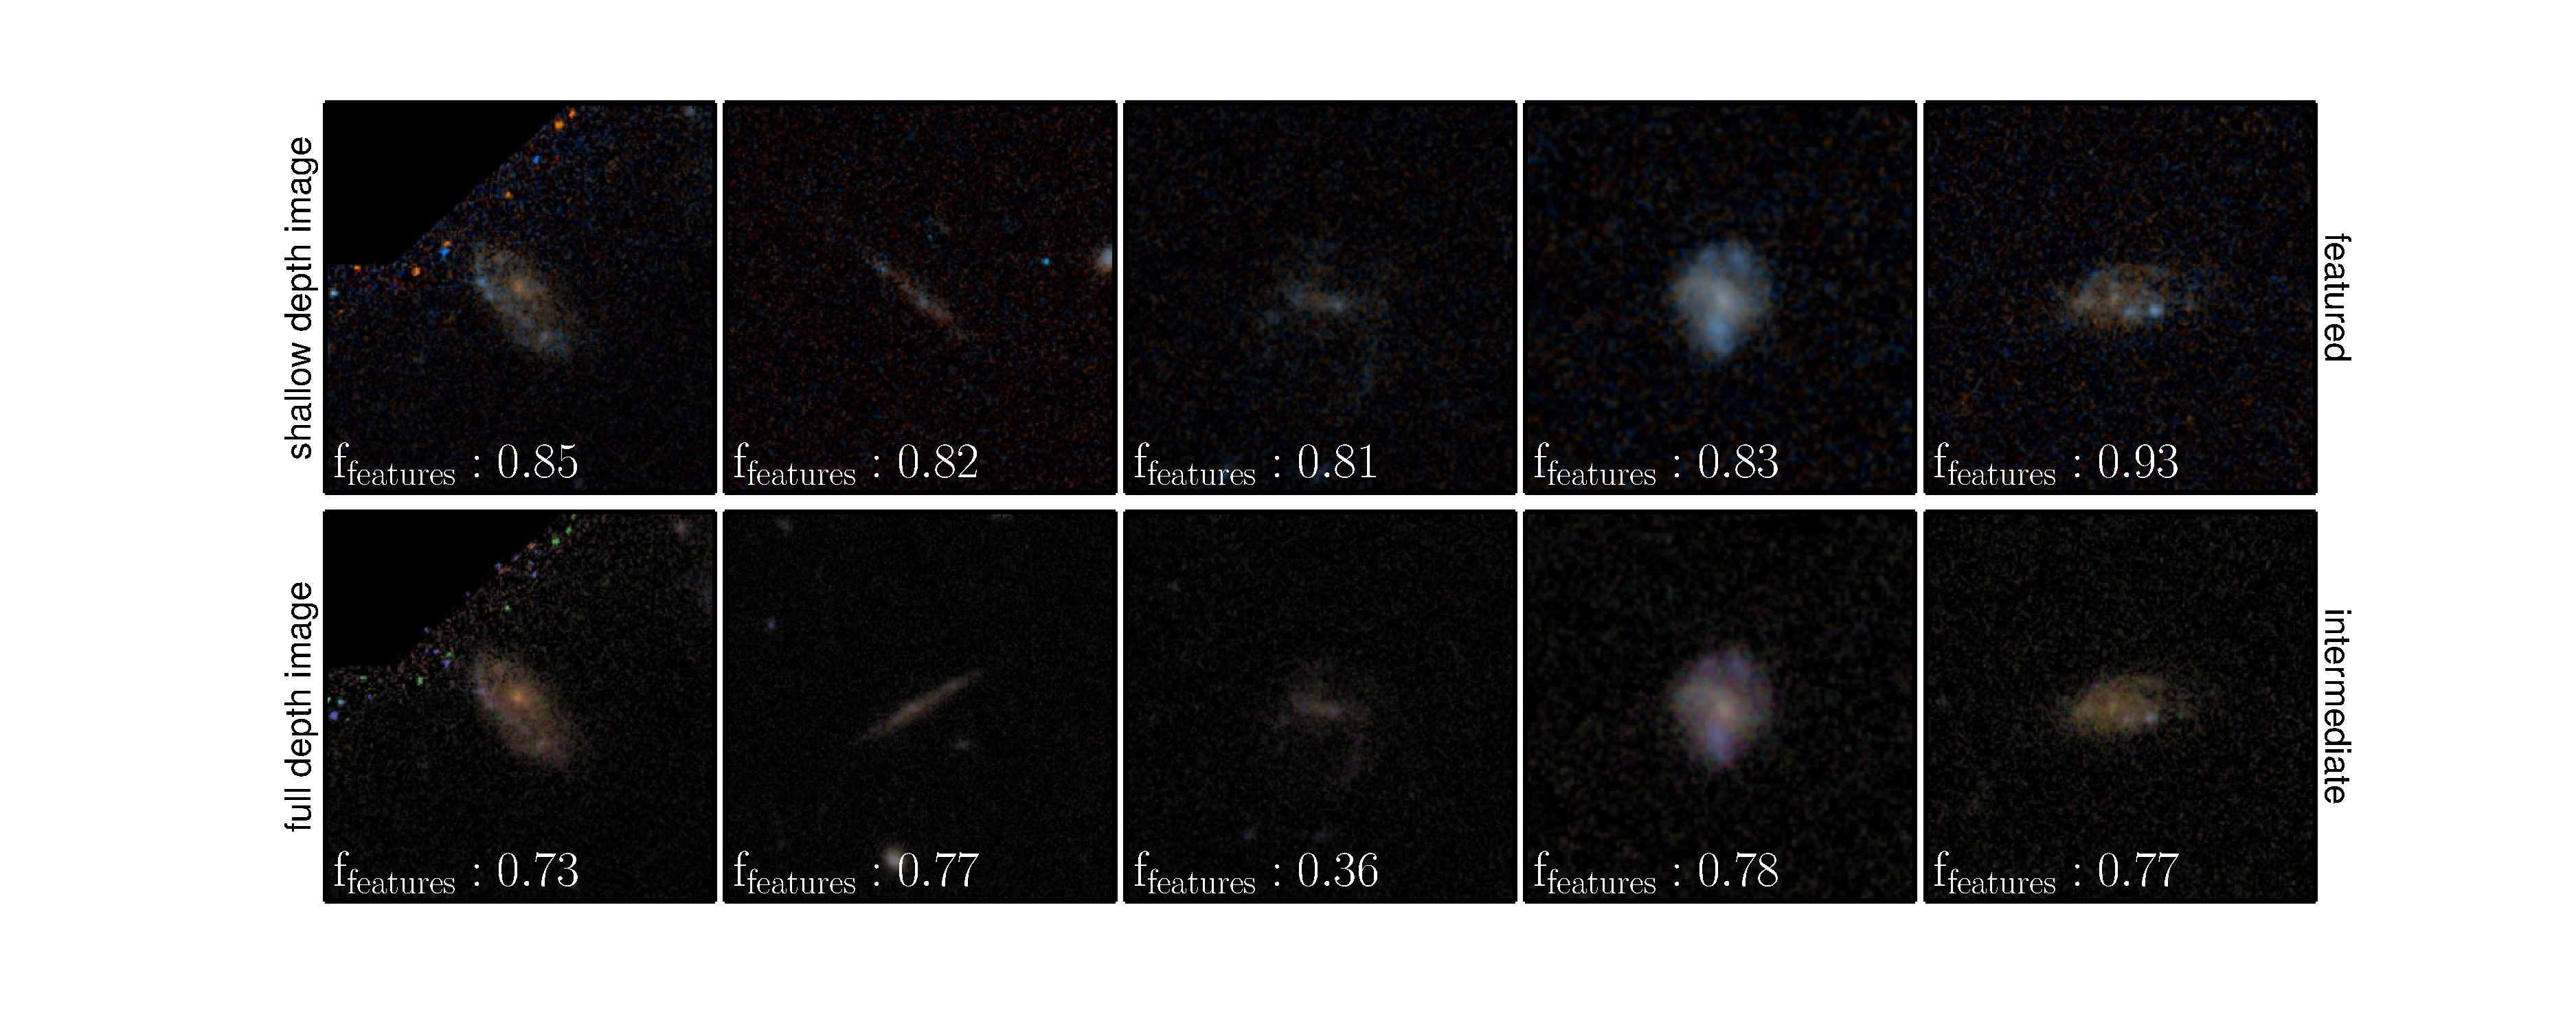
\includegraphics[width=\textwidth]{figures/featured_to_intermediate.pdf}}

\subfigure{[b]\label{fig:featured_to_featured}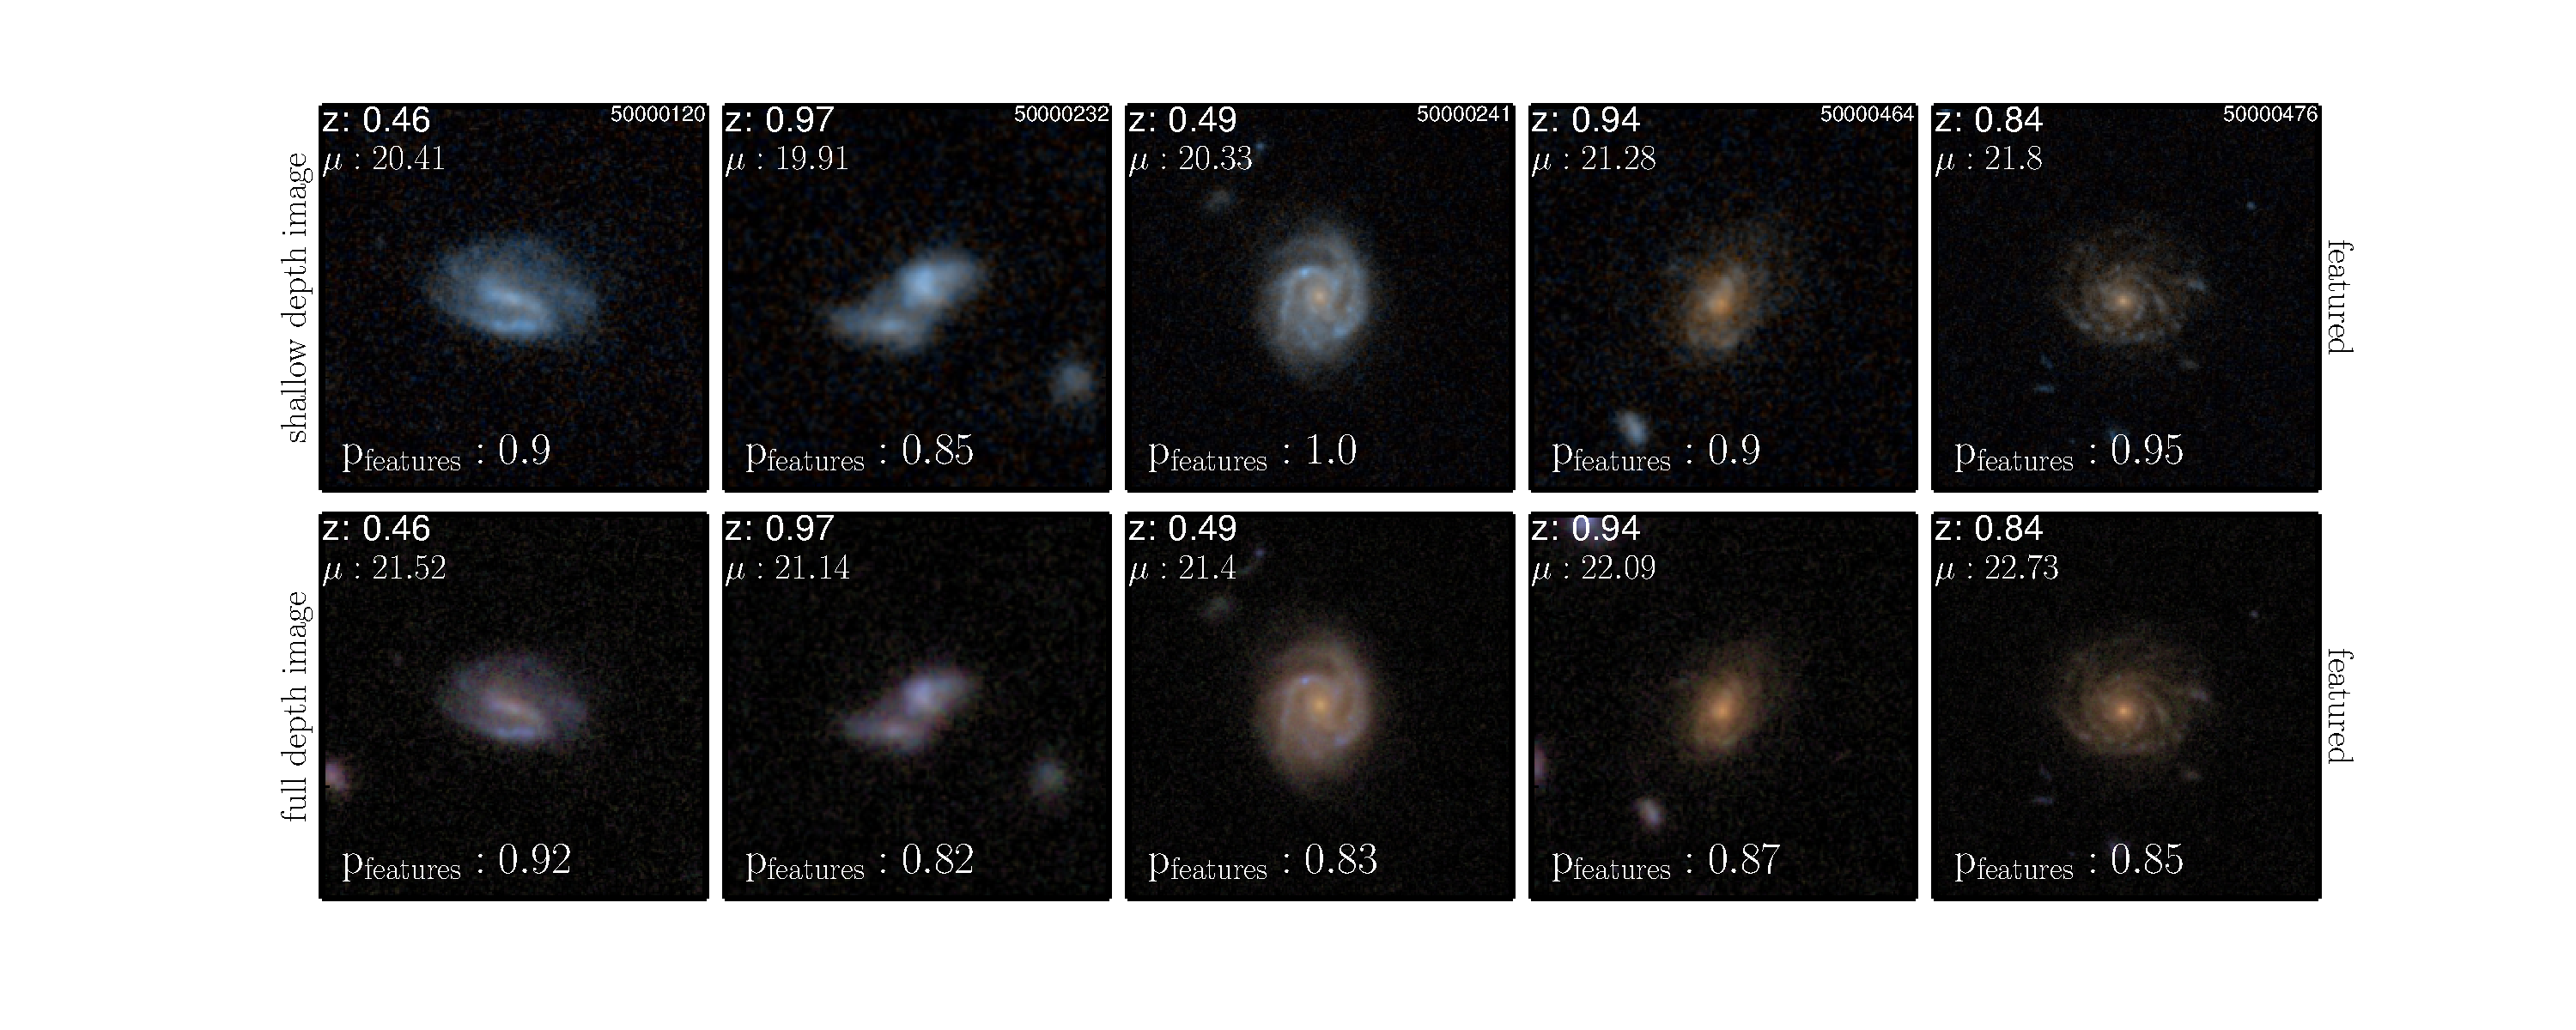
\includegraphics[width=\textwidth]{figures/featured_to_featured.pdf}}


\caption{Galaxies whose shallow images were classified as featured and full depth images were classified as smooth, intermediate, or featured.}
\label{fig:shallow_featured}
\end{figure*}

\subsection{FERENGI analysis of pbar}
\label{sec:ferengi_bar}
\begin{figure*}
\centering
\subfigure{[a]\label{a}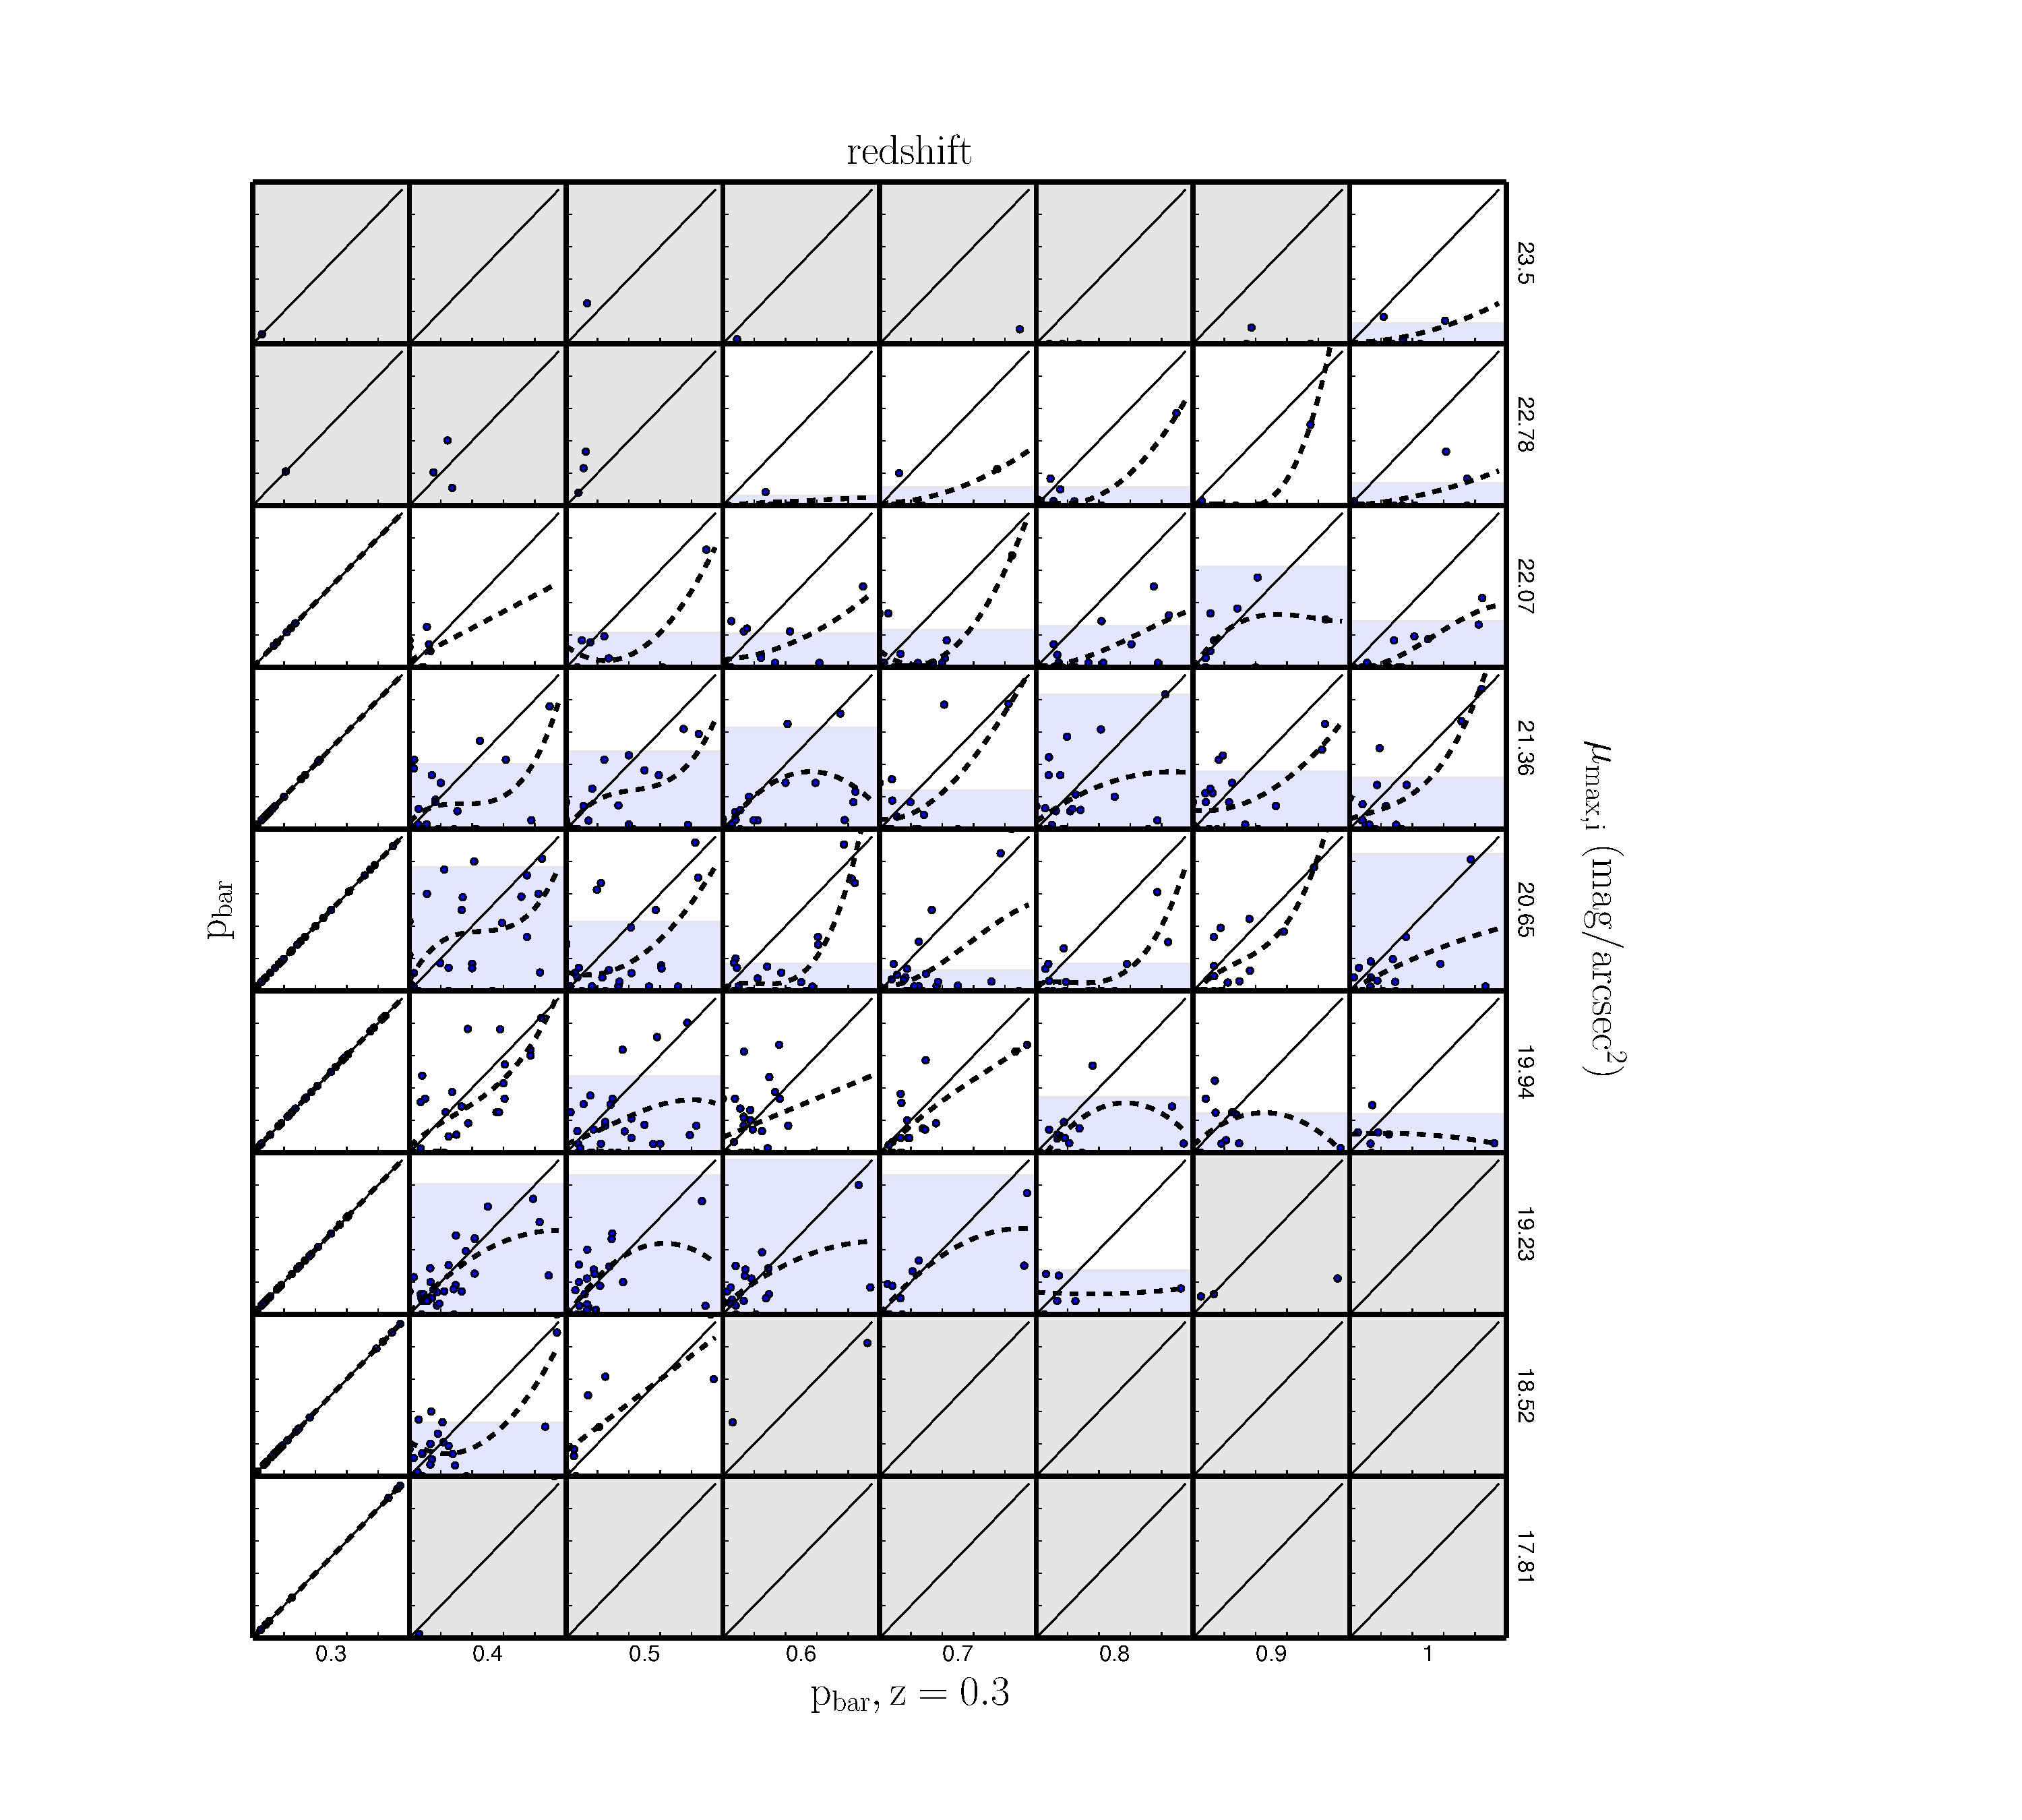
\includegraphics[width=0.5\textwidth]{figures/p_vs_p_SB_redshift_bar.pdf}}
\subfigure{[b]\label{b}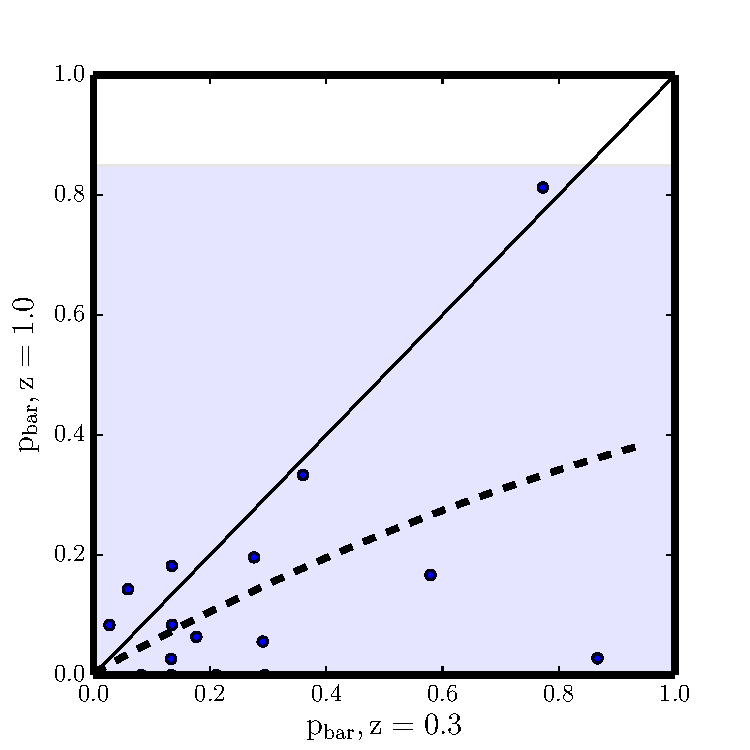
\includegraphics[width=0.4\textwidth]{figures/z1_mu20_subplot1_bar.pdf}}
\\
\subfigure{[c]\label{c}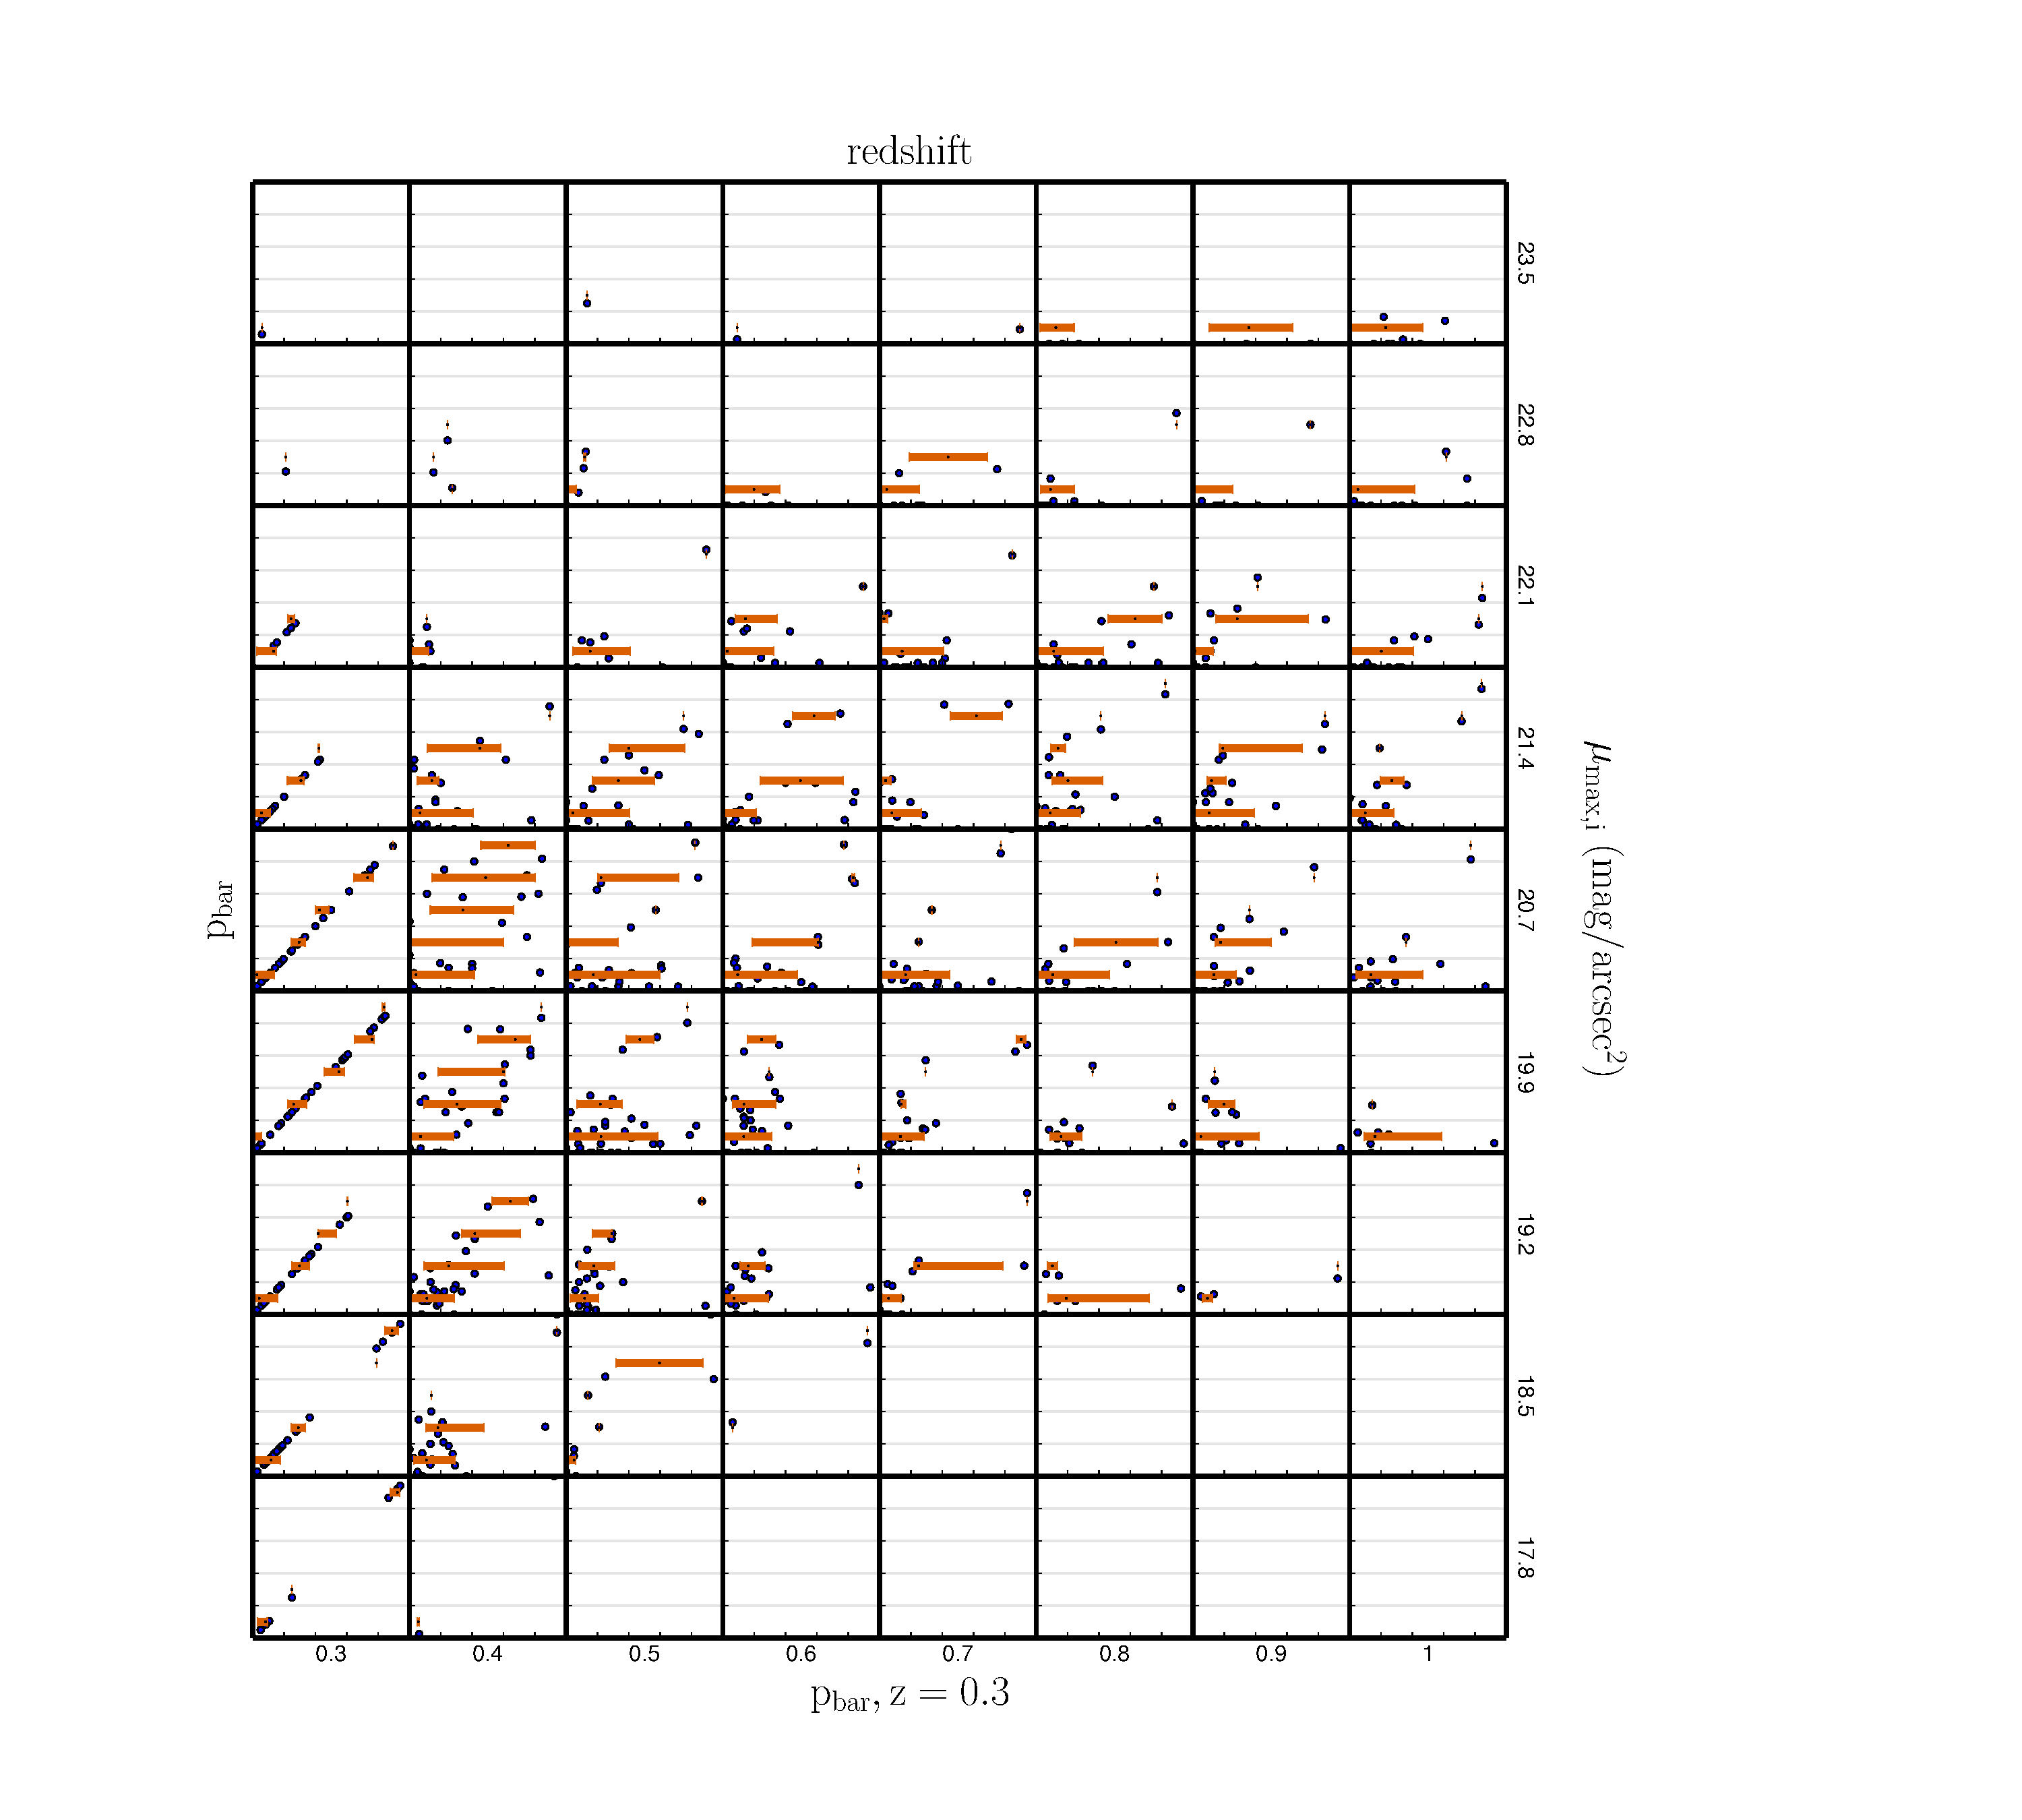
\includegraphics[width=0.5\textwidth]{figures/orangebars_bar.pdf}}
\subfigure{[d]\label{d}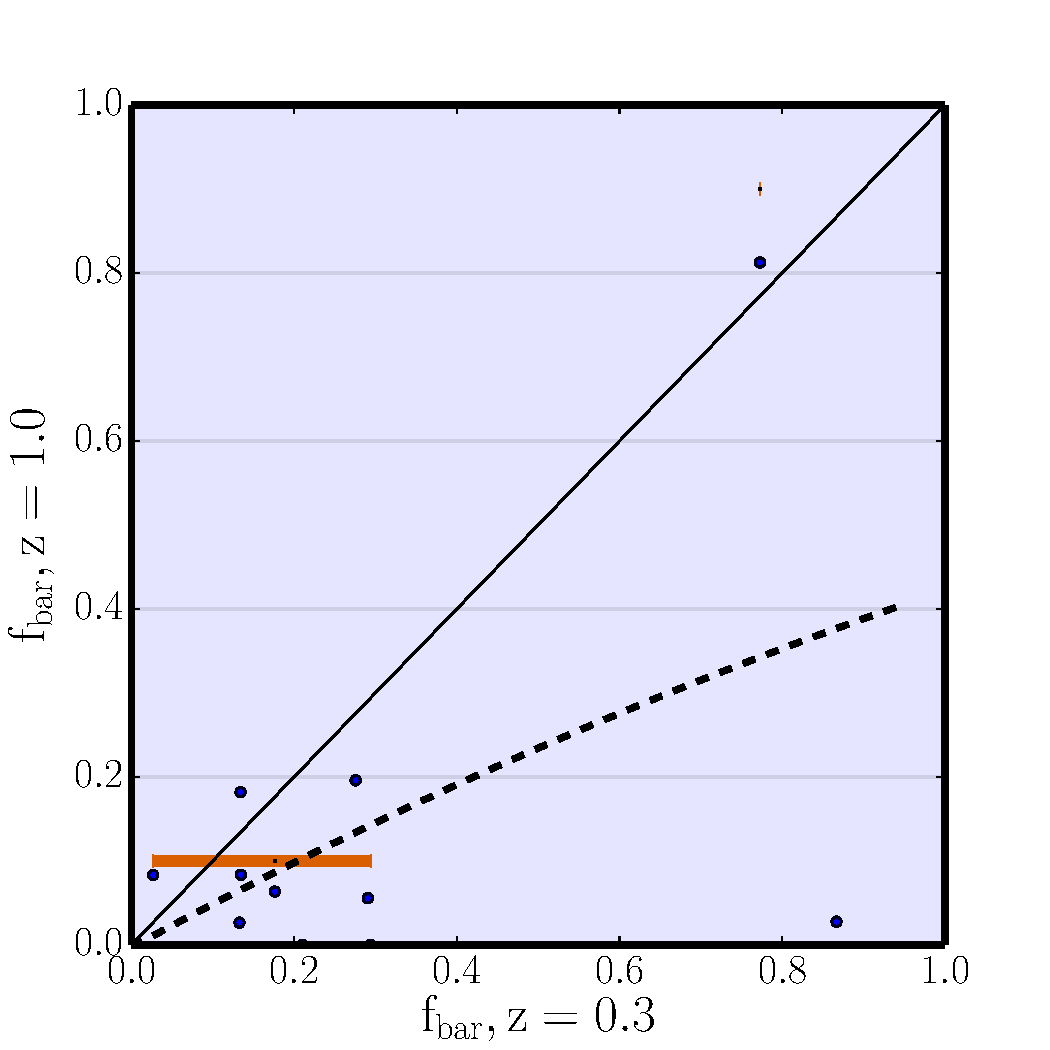
\includegraphics[width=0.4\textwidth]{figures/z1_mu20_subplot2_bar.pdf}}
\caption{Same as Figure~\ref{fig:p_vs_p}, but with the bar question.}
\label{fig:p_vs_p_bar}
\end{figure*}

\begin{table}ー
\caption{Distribution of \ferengi{} images analysed in Figure~\ref{fig:p_vs_p_bar}. Correctable images had a single-valued relationship between their measured \pbar{} values at high and low redshifts (white regions in Figure~\ref{fig:p_vs_p_bar}). Galaxies with a lower-limit on \pbar{} had a non single-valued relationship (blue regions). NEI images had undetermined relationships due to a lack of data ($N<5$) in their corresponding $z$-$\mu$ bins (gray regions). Only 17\% (maximum) of FERENGI galaxies in the sample were considered ``correctable'', which is not sufficient to compute a $\zeta$ function applicable to the Hubble data.   \label{tbl:ferengi_bar_corrections}}
\begin{tabular}{lrr}
\hline \hline
				                   & N       & \% \\
\hline 
Correctable                        & 664   & 17\% \\
Lower-limi                         & 483   & 12\% \\
NEI                                & 2,803     & 71\%\\
Total                              & 3,950   & 100\% \\
\hline \hline
\end{tabular}
\end{table}


\end{document}

